\chapter{绪论}

\section{研究背景及意义}
近年来,推进泵在高速舰船推进系统中得到了广泛应用\cite{Carlton2012Marine}。
随着动力传动系统与船体减振降噪技术的进步,推进泵噪声对舰船总体噪声的贡献度也被相对提高,
因而目前高新船舶对高效低噪声推进泵的需求日益迫切\cite{ozdenUnderwaterRadiatedNoise2016}。
在满足推进性能需求的基础上,
%振动与声学特性目前已成为推进泵优化设计所关注的重点,
推进泵水下噪声已经成为一项关键技术指标。
为了更好的服务于推进泵声学抑制设计,
有必要对推进泵噪声的声纹特征进行研究。
%因此,开展推进泵噪声特性与机理研究对推进泵低噪声设计具有重要意义。
%丰富用于识别推进泵噪声的声指纹特征。

\begin{comment}
推进泵噪声机理较为复杂,抛开空化噪声不谈仅从流致噪声角度考虑,其频谱已呈现宽带与线谱交叠的形貌。
推进泵内非定常流动与水力部件相互作用产生的流致激励是重要的噪声激励源,
推进泵噪声信号中蕴含着丰富的流致激励源信息,流致激励源特征能反映推进泵的运行状态和结构信息。
当推进泵内流动发生显著改变时,其噪声信号的低频声纹理特性也会发生变化。
无论是从特征声源信号识别,或是发展噪声能量主动控制技术角度,
构建推进泵流致激励源识别的有效方法,建立流致激励源特征与噪声信号之间的联系都尤为重要。
\end{comment}

推进泵结构复杂,其辐射噪声场同时存在转子旋转声源,以及定子导管结构的静止声源。
因此推进泵噪声的线谱特征丰富,其中不仅包含有转子叶片离散线谱信息,同时也包括
动静相互作用的影响。
噪声的特征线谱是推进泵噪声研究中所关注的重点,
特征线谱不仅能表征推进泵的工作状态和结构信息,
也是声呐系统追踪和识别的重要信息。
%但是其提取面临环境干扰强、直接测量难度大的问题。
%噪声的特征线谱不仅能表征推进泵的工作状态和结构信息,
%当监测和识别推进泵水声目标信号时,噪声的特征线谱
%也是声呐系统追踪和识别的重要信息。
%推进泵噪声的特征线谱已成为噪声研究所关注的重点。
但是由于复杂环境声场对推进泵辐射噪声的干扰,
监测系统接收到的目标声场信号的信噪比较低,
传统的频谱分析方法已无法实现噪声中特征线谱的准确识别。
%无论是复杂环境声场对推进泵辐射噪声的干扰,还是推进泵本身因流动特征改变而导致的声学特征改变,
%都决定了推进泵声纹特征信号存在多样性和复杂性\cite{__2016杨琼方}。
%基于上述因素,
%其次,推进泵噪声存在显著的调制特性,形成了调制特征线谱,调制现象包含着丰富的流场信息。
%传统的噪声特征提取方法,如频谱分析等,具有抗噪性能较差,难以提取弱信号特征等缺点,
%无法实现噪声中特征线谱的准确识别。
因此,无论是从水声信号识别,或是推进泵声学抑制设计角度,
开展推进泵噪声的特征线谱提取技术研究具有重要意义。

\begin{comment}
%对声指纹特征内涵的挖掘具有重要意义。
传统的频谱分析方法已经无法准确的对流致激励特征声源进行识别,以及对推进泵的运行状态进行表征。
其噪声信号中存在复杂的干扰因素:其一,推进泵处在复杂的背景环境声场中,
动力系统等辅助结构产生的辐射噪声也给目标声源信号带来了很大干扰,影响
测试系统对推进泵目标真实辐射噪声信号的监测;其二,推进泵结构复杂,
推进泵辐射噪声场同时存在转子旋转声源,以及定子导管结构的静止声源,
其辐射噪声具有分量复杂性。基于上述因素,监测系统接收到的目标声场信号的信噪比较低。特征信
号如流致激励源特征频率、轴频等与其他背景噪声相比均较为微弱,
给基于传统噪声特征提取方法带来了困难,难以准确的识别噪声信号的流致激励源特征。
其次,推进泵噪声存在显著的调制特性,调制现象包含着丰富的流场信息,
但是传统的频谱分析及解调方法无法实现高精度低频调制特征的提取。
因此,开展低信噪比工况下的推进泵噪声信号的低频特征提取技术研究
有重要的理论和工程意义。
\end{comment}

基于以上背景,本文围绕推进泵噪声的声纹特征分析和特征线谱识别展开研究。
首先,从推进泵的噪声试验研究出发,本文基于LabVIEW平台开发了推进泵噪声测试与分析系统,
实现了推进泵噪声的测量和实时分析,为推进泵噪声的声纹特征分析奠定了研究基础。 
其次,以紧凑型前置导叶的单级推进泵和新型结构的双级推进泵为研究对象,
在大型空泡水洞中对其开展噪声试验研究,
获得了推进泵在不同水动力性能工况下的噪声数据。
研究了不同工况下推进泵噪声的声纹特征变化,以及流速等与噪声的声学关联性,
探讨推进泵噪声的声纹特征。
最后,从推进泵噪声的特点出发,开展对其噪声信号的组分研究,
基于推进泵噪声信号的循环平
稳特性,引入了二阶循环统计量提取了试验噪声信号中的低频线谱。
同时联合数值模拟中提取的非定常脉动力特征,验证了循环平稳分析方法的可行性,
并进一步分析了推进泵噪声的调制特性。

\begin{comment}

目前针对推进泵流致激励特性的研究已经开展了大量工作,研究主要集中通过数值模拟获取
压力脉动特性、激振力特性等方面,难以通过试验精确获取流致激励源特征。
其中蕴含着丰富的流致激励
源信息,但是传统的频谱分析及解调方法无法实现高精度低频调制特征的提取。

\end{comment}

\section{研究现状}
\subsection{噪声测试与分析技术研究现状}
\begin{comment}
水下环境噪声数据采集装置对于水声试验来说是不可缺少的,因此设计
一套高性能的、能够适应水声信号特点的数据采集
系统十分必要。水声信号在水中传播时,水中的自然
环境极其复杂,要求所采用的数据采集器能够适应水下恶劣的自然环境,不但具有较大的动态范围,
所采集信号的幅度范围要尽可能宽,而且试验现场的数据量很大,常常需要多通道同步进行数据采集,
这样,对数据采集器提出了很高的要求。另外,从节约成本的角度考虑,又要求所采用的系统应该具有
一定的通用性和灵活的扩展能力。文中所要完成的
工作正是基于这一目的而展开的。

随着测试技术的发展,目前对传统的复杂仪器,分析方法的依赖性在减少,而正在流行着一种 
将计算机技术和噪声测试技术相结合、组建虚拟噪 
声测试系统的方法,即将虚拟仪器技术的测试技术 
引到噪声测试领域中,借助计算机软件技术来设计 
噪声分析软件。


\end{comment}
随着测试技术的发展,将计算机技术和噪声测试技术相结合、组建虚拟噪声测试系统的方法,
即虚拟仪器测试技术在噪声测试领域中被广泛应用\cite{yu2018}。利用虚拟仪器技术,
用户可根据实际测试的要求来自定义仪器的功能,实现测试数据的处理,
从而可提高测试任务的运行速度效率\cite{tang2021}。

国内外在噪声测试系统研究方面做了不少工作,
%市场上涌现出面对机器设备、电子器件、海底环境等众多方向的较多功能丰富的振动噪声测试、采集和分析系统的产品。
国外对虚拟仪器的研究开始很早。其中美国NI公司最具有代表性,
其生产的NI-PCI、NI-USB等型号在数据采集模块领域拥有较大部分的市场,
开发的虚拟仪器软件LabVIEW也成为虚拟仪器开发的主要编程工具\cite{2007Labview}。
此外还有丹麦B\&K公司的各类传感器硬件,LDS振动噪声测试系统;德国申克公司的SCHENCK在线振动与噪声检测系统;
英国DI公司的RT440振动噪声系统等也应用广泛\cite{dingJi2014}。
这些产品大都向着多功能多用途、通用化和智能化发展,
针对不同领域的分析需求涵盖了振动噪声综合测试、设备运行状态监测和结构模态分析等方面。
但是这些产品也存在一些局限性,比如价格昂贵,操作复杂,不便于维护,
在国内缺少汉化版而使用不便,从而难以在基层推广\cite{boMeasurementSystemWind2011}。

国内对于噪声测试分析系统的研究起步较晚,从八十年代大力发展之后,
许多企业和高校单位也相继研制出各种噪声测试分析系统\cite{jiangJi2020,sun2020}。
目前国内在数据采集卡和上位机分析软件的结合方面主要采用的方式有两种,一
种是自行购买数据采集卡,然后自行设计上位机分析软件。这种方案价格低廉,具有灵活的扩展能力,
但是自行开发上位机软件周期长。
如肖艳华等\cite{xiaoJiYu2017}构建了一种以LabVIEW为软件平台的多通道噪声倍频程分析系统。
余世策等\cite{余世策2016基于虚拟仪器的噪声测试系统研发}采用NI通用数据采集卡和声压传感器搭建了通用噪声测试系统,
利用LabVIEW的mathscript节点设计了噪声测试、 FFT分析、1/3倍频程分析以及计权网络对声级的调整等功能。
靳雪莲等\cite{jinxuelian2010}设计了一套基于虚拟仪器和图形化编程语言LabVIEW的水下环境噪声采集系统并加以实现,
可以实现水下环境噪声的长时间连续采集。

另一种是购买专业公司
的数据采集卡和配套的上位机分析软件,这种套件通用性强,但是
操作复杂,分析功能有限不容易扩展,且价格比较高昂。
如大连理工大学研制的 PDM2000 数据采集分析仪;哈尔滨工业大学研制的 MMMD 系列分析系统;
西北工业大学研制的 MD3905系统;北京东方所研制的DASP和INV系列数据采集分析产品\cite{dingJi2014}。
这些产品实现了集数据采集、信号处理、振动分析、模态测试和响应计算等多种功能于一体,
但是在性能指标、可靠性等方面均存在一定的局限性。

%综上,现有的噪声测试与分析系统在推进泵噪声的实际试验中,存在操作复杂,分析功能有限不容易扩展等局限性,
%为满足系统在实际试验中应具有的便携式和高效率等特点,开发一套测试采集系统对推进泵声纹特征的研究有重要意义。
\subsection{推进泵噪声研究现状}
目前,国内外已经围绕螺旋桨、对转桨、推进泵等多种类型推进器的辐射噪声开展了研究,
在噪声机理、特性与预报方面已有较多研究成果。
螺旋桨直接辐射噪声按声源类型的不同分为流致噪声和振动噪声,其无空化噪声按频谱特性可分为低频线谱噪
声、低频宽带谱噪声和高频宽带谱噪声\cite{cheng2019,xuye2019a}。
目前使用FW-H方程预报螺旋桨、对转桨等推进器低频线谱噪声的技术已比较成熟,
Seol、Gennaretti等学者采用时域声类比方法预报了无空泡及空泡螺旋桨噪声,采用面元法得到桨叶时域压力,将其作为声源输入FW-H方程预报远场声辐射\cite{seol2002,gennaretti2012}。
常欣等\cite{changxin2018}基于非定常面元法研究了对转桨的无空泡噪声特性,分析了桨叶数、桨直径、前后桨间距、伴流场等与对转桨无空泡噪声的声学关联性。
熊紫英等\cite{xiong2014}对船舶无空泡螺旋桨非定常推力脉动及其诱导的线谱噪声进行了研究,基于速度势面元法计算得到非均匀流场中无空泡螺旋桨的推力脉动,
验证了螺旋桨非定常推力脉动理论预报方法。

随着计算机计算能力的不断提高,以LES为代表的CFD方法在声源求解上的应用越来越广泛,
同时声学边界元法也为推进器噪声预报提供了一种新的途径。
杨琼方等\cite{__2016杨琼方}通过脉动力源线谱特征预报了对转桨的线谱频率和幅值,
结合数值模拟和声学边界元法预报了宽带噪声,分析了对转桨压力脉动、噪声频谱特征等。
鲁利等\cite{鲁利}将RANS、DES和LES三种方法得到的脉动压力作
为声源,结合声学边界元法预报螺旋桨噪声,计算结果表明低频线谱噪声是螺旋桨总噪声的主要贡献者。
Blake等学者提出的以谱方法为基础的条带数值法是螺旋桨低频宽带谱噪声主要研究手段\cite{1986Mechanics,jiang2020}。
朱锡清等\cite{朱锡清2006}在风洞中测量了船尾模型螺旋桨盘面处的湍流场特性,计算了某船在不同航
速下的低频宽带噪声级,并指出航速、螺旋桨直径、转速、弦长、叶片数与宽带噪声级的声学关联性。
Zeng等\cite{zeng2017,zeng2020a}分析了水下对转桨无空化辐射噪声的调制机理,建立了水下对转桨无空化噪声的调制模型,在空泡水筒试验中验证了其辐
射噪声调制机理。

相比螺旋桨、对转桨等推进器,推进泵结构更加复杂,同时具有内、外流动。
在有关推进泵噪声机理和辐射噪声数值预报研究等方面,由于推进泵的低噪声特性
与舰艇隐身性密切相关,其军事应用背景敏感,国外相关的公开文献几乎不可见。

在螺旋桨和对转桨噪声的研究基础上,国内学者对推进泵噪声展开了大量研究。
彭临慧等\cite{__1998彭临慧}对推进泵进行了低频线谱的实验研究及分析结果。
实验发现推进泵的噪声谱中,存在及其丰富的低频线谱,
线谱的谱级可比噪声谱中连续谱部分高出20-30dB,这些低频线谱基本上都是转子轴频和叶频的谐波分量。
赵兵等\cite{__2009赵兵}对鱼雷-推进泵耦合模型进行了流动干涉发声机理的研究,采用Proudman 声学近似方法
初步分析了其声源强度分布,得出鱼雷泵喷主要噪声源分布与流动干涉发声原因。
周友明等\cite{__2011周友明}较为全面的分析了几何参数对泵喷流噪声水平的影响,采用作用于推进器的径向力的脉动幅值来
衡量线谱噪声水平,采用 Proudman 提出的声功率来衡量推进器的宽带噪声水平,发现推进器几何参数与噪
声水平之间存在明确的关系和规律。
刘敏等\cite{__2011刘敏}通过采用有限元方法分析了推进泵声场声压分布、声压指向性,得到导管在低频段对噪声影响小,而在高频段降
低噪声声压级并改变指向性的关键结论。
卢丁丁等\cite{__2016卢丁丁}基于点源模型理论和边界元计算方法,计算了推进泵导管内转子声场,
分析表明导管对径向测点处转子声场影响较大,对轴向测点处转子声场的影响可以忽略。
高丹妮等\cite{__2018高丹妮}采用大涡模拟及耦合有限元/边界元数值方法,计算了推进泵声振耦合响应,
结果表明导管内壁脉动压力最大值集中在转子区域,流体激励力特
征频率出现在叶频及其倍频处。
苏永生等\cite{__2013苏永生}分析了喷水推进泵空化噪声的调制特征,并研究了空化程度与噪声的关系。
杨琼方等\cite{__2016杨琼方}基于声学边界元方法预报了泵喷无空化辐射噪声的低频线谱和宽带谱,
可得到泵喷低频线谱频率和幅值信息。
丁丰宁\cite{__2019于丰宁}基于数值计算预报了流体激励力作用下推进泵流体辐射噪声与结构辐射噪声,并分析了其噪声特性。
Du等\cite{duNumericalAnalysisFlow2019a}基于数值模拟预报了推进泵不同转速下的噪声声源分布,以及监测位置、转速与噪声总声压级的声学关联性。
Qin\cite{qinUnderwaterRadiatedNoise2019a}和Sun\cite{sunNumericalInvestigationNoise2019}分别对带锯齿型导管的推进泵噪声进行了预报,并对锯齿型导管的降噪机理进行了分析。

总的来说,推进泵噪声机理复杂,声纹特征丰富,
噪声信号中不仅包含有转子叶片的离散线谱信息,同时也包括动-静相互作用的影响。
目前对推进泵噪声的研究主要集中在低频线谱噪声特征频率、声指向性等噪声特性上,研究手段以理论计算和数值模拟为主,
推进泵声纹特征的内涵有待于进一步研究。

\subsection{循环平稳信号分析手段}
推进泵等旋转机械周期运转的方式使其噪声信号具有周期特性,同时由于实际运转状态存在很
多随机因素,从而使得其噪声信号兼顾周期性和随机性的特点,因此推进泵噪声信号可
以归于循环平稳的范畴\cite{陈进2013机械故障特征提取的循环平稳理论及方法}。
针对旋转机械监测信号特征提取的算法,国内外学者做了广泛的研究,
主要的信号解调方法有包络解调、谱峭度分析、循环平稳分析方法等\cite{wangSpectralKurtosisFault2016}。
在实际应用中包络解调应用最为广泛,现场的特征提取方式多采用该算法,
但是该方法的抗噪性能较差,弱信号的调制特征提取比较困难\cite{abboudEnvelopeAnalysisRotating2017,2014The}。
谱峭度分析方法是在包络解调算法的基础上发展而来,其更注重共振频带的识别,
对调制特征的提取依然为包络解调,因此该算法降低了解调谱中存在的干扰,
但是其弱信号的提取能力依然较差\cite{2007Fast,2011A}。
循环平稳分析方法是一种基于高阶统计量的特征提取算法,
该方法具有较好的抗噪性能\cite{gardnerCyclostationarityHalfCentury2006,songRobustPassiveUnderwater2019}。

近年来,循环平稳分析方法开始用于机械故障检测以及旋转机械信号特征提取领域\cite{2006Detecting,poirierExtrapolationDynamicLoad2017,fengGearDamageAssessment2011,何俊2007,antoniCyclicSpectralAnalysis2007a,2017Extrapolation}。
基于二阶循环平稳性的分析方法是高阶统计量中旋转机械特征信息提取的最有效手段\cite{antoniUseCyclicPower2005}。
Boungou等\cite{boungouFatigueDamageDetection2015}利用二阶循环平稳分析方法用于不锈钢在周期性
载荷作用下内部疲劳损伤的特征提取和探测,并实现了故障特征的准确识别。
学者Antoni等\cite{antoniCyclostationarityExamples2009}对循环平
稳信号的分析方法进行了详细的应用研究,并利用旋转机械信号实例对循环平稳分析方法实现特征提取的
有效性进行了验证。
此外,Antoni建立了旋转机械振动信号的循环平稳摸型,并提出了分析旋转机械信号的一般方法,
引入了循环密度谱成功提取了旋转机械实例信号中的特征频率\cite{antoniCyclostationaryModellingRotating2004a}。
李诗佯等\cite{2019Cyclostationary}人将CFD(计算流体力学)方法和循环平稳分析方法相结合,
建立了离心泵振动信号的幅值调制模型,有效的从振动信号中提取出流致振动激励特征。
循环平稳分析方法也被应用于螺旋桨的辐射噪声信号的解调,能
够有效的用于螺旋桨的状态特征提取和目标识别\cite{antoniDetectionSurfaceShips2012,2016Cyclostationary}。
Rajan等\cite{rajanCyclostationarityBasedSonar2016}分析了螺旋桨噪声的幅值调制特征,
基于其循环平稳特征识别了叶片数和轴频等声纹特征,验证了循环平稳分析方法的抗干扰性。

总的来说,对于信噪比低的旋转机械信号,例如处于复杂水声环境中的推进泵噪声,
循环平稳分析具有较好的解调能力和抗噪性。

\section{研究目标和内容}
%非均匀流场与泵相互作用产生的非定常负载和压力脉动是推进泵流致激励的内在表现。
本文围绕推进泵噪声的声纹特征研究展开,针对噪声特征线谱提取的需求,
以紧凑型前置导叶的单级推进泵和新型结构的双级推进泵为研究对象,
设计噪声测试与分析系统并开展试验研究,
研究了推进泵噪声的声纹特征,
基于循环平稳分析方法实现了推进泵噪声的特征线谱提取。
为实现本文的研究目标,本文主要章节研究内容如下所示:

第二章,针对目前噪声测试与分析系统存在操作复杂、信号分析效率低等问题,基于推进泵声纹特征分析的需求,
结合LabVIEW平台开发了推进泵噪声测试与分析系统。其中涵盖了实现信号采集的硬件系统设计,
以及实现信号分析和存储的软件系统设计。
首先,介绍了推进泵噪声试验平台和测试基本参数,以及噪声特性的分析需求,
制定了噪声测试与分析系统的技术框架和系统方案;
其次,阐述了系统的硬件组成、传感器型号及参数,研究了数据采集卡的系统结构和传输过程,
对硬件与计算机的交互通信进行了说明;
最后,对软件系统的各个功能模块进行了设计,
对信号采集模块、信号分析模块、数据管理模块等进行了详细说明。
该系统为开展推进泵噪声的试验研究奠定了研究基础。

第三章,
以紧凑型前置导叶的单级推进泵和新型结构的双级推进泵为研究对象,在大型
空泡水洞中对其分别开展了噪声试验。
首先,本研究对多工况下的水
洞背景噪声进行了试验测量,分析了水洞背景噪声的频谱能量分布特点和特征频段总声压量级等声纹特征,
讨论背景噪声对推进泵噪声的影响;
其次,采集了单级推进泵和双级推进泵在不同水动力性能工况下的噪声数据,基于噪声采集与分析系统的分析模块,
借助频谱分析和三分之一倍频程分析等信号分析手段对推进泵噪声数据进行处理。
在考虑背景噪声影响的基础上,研究不同工况下
推进泵噪声的声纹特征变化,以及流速等与噪声的声学关联性,探讨推进泵噪声的声纹特征。

第四章,开展了推进泵噪声信号的特性研究。基于推进泵噪声信号的特点,对噪声信号进行了组分分析、循环平稳特性、调制模
型的研究。首先,结合推进泵噪声信号产生的机理,将推进泵噪声信号分量分为确定性信号分量、
调制信号分量和噪声信号分量,并对各分量的统计
特征进行分析研究;其次,基于推进泵噪声信号的循环平稳特性,对一阶循环平稳统计量和
二阶循环平稳统计量进行了介绍,为噪声信号的预处理和调制信号的解调算法提供理论基础。
最后,结合推进泵噪声信号特征,
对匀速运转工况下的无空化噪声信号建立了幅值调制信号模型,采用循环平稳
分析方法对噪声信号的仿真模型进行了研究,验证了循环平稳解调算法提取多组分调制
频率的有效性和良好的抗噪性能。

第五章,
推进泵噪声的特征线谱提取和分析。针对噪声的特征线谱提取的需求,
首先,基于循环平稳分析方法实现了推进泵低频线谱成分的提取;
其次,采用 CFD 数值模拟获得了推进泵脉动力特征,
结合循环平稳分析方法的低频线谱提取结果和非定常脉动力的特征线谱,
验证循环平稳分析方法提取特征线谱的可行性;
最后,对推进泵噪声的调制特性进行了研究。
\chapter{推进泵噪声测试与分析系统设计}
\section{引言}
针对目前噪声采集与分析系统操作复杂、分析效率低等问题,基于推进泵声纹特征分析的需求,
本研究结合LabVIEW平台开发了推进泵噪声测试与分析系统。其中涵盖了实现信号采集的硬件系统设计,
以及实现信号分析和存储的软件系统设计。系统支持同步对多通道传感器信号实时采集,各通道信号同时处理、显示及存储。
经过试验测试,该系统可显著提高测试和分析任务的运行效率。

基于此平台可开展对噪声信号时域分析、频谱分析、三分之一倍频程和特征频段分析等研究,
为进行推进泵噪声的声纹特征分析奠定了研究基础。
\section{系统总体设计概述}
\subsection{推进泵试验台简介}
本研究依托上海船舶运输研究所(SSSRI)的空泡水洞,针对推进泵样机模型开展了噪声性能的试验研究。
空泡水洞由德国KEMPF\&REMMERS公司制造,如\autoref{fig:tube1}和\autoref{fig:tube2}所示。
水洞整体采用不锈钢材料,配有压力调节箱和除气装置,具有很好的可控性。
水洞工作段长2.6m,横截面呈方形带圆角,尺寸为0.6m×0.6m。
\begin{figure}[htbp]
    \centering
    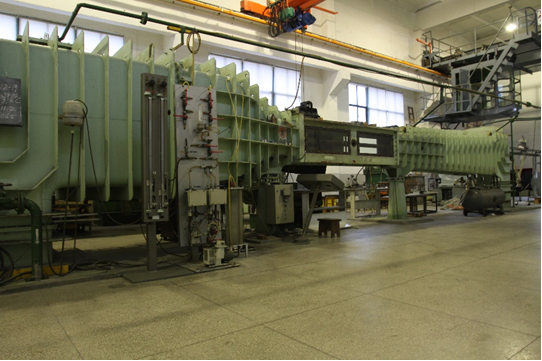
\includegraphics[scale=0.65]{3水洞1.png}
    \caption{\label{fig:tube1}SSSRI空泡水洞}
\end{figure}
\begin{figure}[htbp]
    \centering
    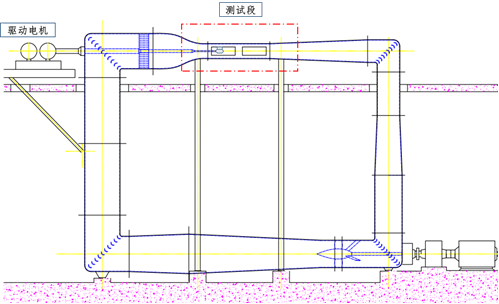
\includegraphics[scale=0.75]{3水洞2.png}
    \caption{\label{fig:tube2}水洞整体结构}
\end{figure}

水洞工作段如\autoref{fig:work}所示,最高水速可达12m/s。
缩比模型样机悬挂于水洞上壁面,导管由光折射率与水一致的透明有机玻璃制成,以确保其内流场的可视性。
水筒侧面有机玻璃外安装一小型水舱,将水听器置于其中,测量推进泵在多工况下运转的水下噪声。
\begin{figure}[htbp]
    \centering
    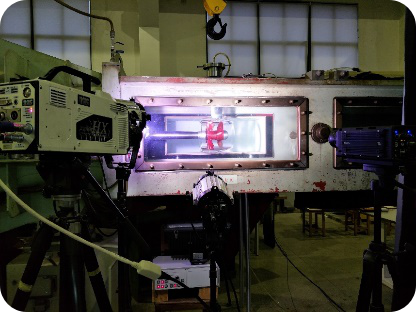
\includegraphics[scale=1.0]{3水洞工作段.png}
    \caption{\label{fig:work}水洞工作段}
\end{figure}

水洞的水动力测试系统采用安装在传动轴上的动力仪测量叶轮和导流锥上产生的推力和转矩,
动力仪测量的最大推力为3000N,最大扭矩为150N$\cdot$m,测量精度0.2\%,最大转速4000rpm,能满足推进泵模型的测试需求。
采用五分量测力天平测量导管和导叶等静止部件的受力情况。
水洞内的水速、压力信号和动叶的推力、扭矩和天平信号经放大器放大后送计算机进行A/D转换并处理,转速信号通过频率计同步输入计算机。

为了分析推进泵在不同水动力性能下的噪声特性,对推进泵的水动力特性和水动力噪声同时进行了测量。
在噪声试验方面,采用水听器作为声学传感器。
由于推进泵声信号覆盖了从几百到几千赫兹
的频率范围,因此要求选用的水听器具有良好的低频响应性能。实验中,水听器采用型号
为丹麦 Reson TC4013,该水听器的有效频率范围为 1Hz-170kHz,
基本信息如\autoref{tab:stq}所示,该水听器具备良好的灵敏度和全指向性
能,可以确保各个方向的声音都有同样的高灵敏度和传导精度,能够满足推进泵水下噪声信号频带宽度与数据采样率的需求。
\begin{table}[htbp]
    \centering
    \caption{\label{tab:stq}水听器基本信息}
    \begin{tabular}{cc}
     \toprule
     指标&范围\\
     \midrule
     工作频率&1 Hz$- $170 kHz\\
     接收灵敏度&-211 dB$\pm$ 3 dB\\
     最大操作水深&700 m\\
     操作温度&-2℃$- $80℃\\
     \bottomrule
    \end{tabular}
\end{table}

推进泵噪声测试系统的示意图如\autoref{fig:equipment}所示,主要包括测试推进泵、水洞、水听器、
数据采集卡、电脑(上位机软件)五部分组成。
\begin{figure}[htbp]
    \centering
    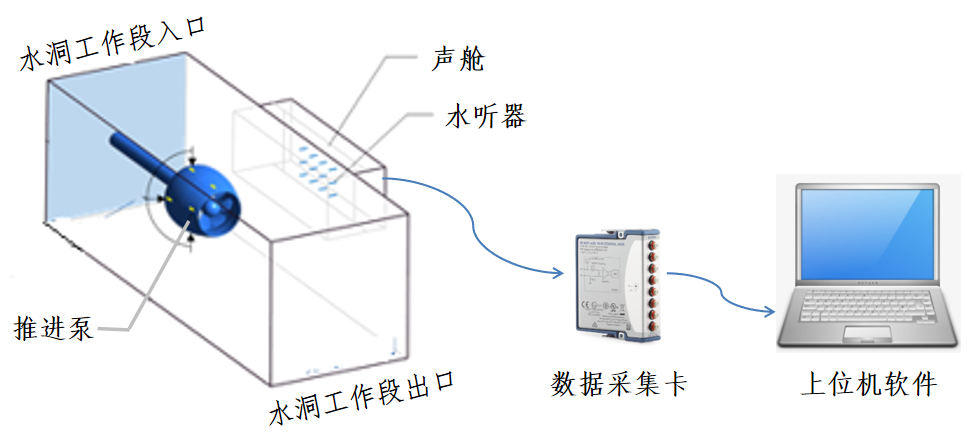
\includegraphics[scale=0.55]{3测试系统1.png}
    \caption{\label{fig:equipment}推进泵噪声测试系统装置示意图}
\end{figure}

\subsection{测试基本参数和数据处理}
本研究设计的测试信号对象为声压,用来表征测试对象的声学性能,可由水听器进行测量。
为了分析推进泵噪声的总声压量级、频谱能量分布
等声纹特征,在数据处理方面,主要涉及频谱分析、1/3倍频程分析和特征频段的总声压级分析。

在噪声信号的分析中,声压级是常用的参数,一个声学量的级是该量与同类量的基准值之比的对数。
其中,声压级定义为将待测声压$p_e$与参考声压$p_{ref}$的比值取常用对数,再乘以20,以分贝计,即
\begin{equation}
    \label{equ:p}
    L_{p} = 20\log_{10}{\left(p_{re}/p_{ref}\right )}
\end{equation}

式中,在水中基准声压为$p_{ref}= 1\times 10^{-6} \mathrm{P} a$,在空气中基准声压为$p_{ref}= 2\times 10^{-5} \mathrm{P} a$。
\begin{comment}
同理,振动加速度级也定义为加速度有效值$a_e$与基准加速度$a_{ref}$之比的以10为底的对数,再乘以20,以分贝计,即
\begin{equation}
    \label{equ:a}
    L_{a} = 20\log_{10}{\left(a_{re}/a_{ref}\right )}
\end{equation}
式中,基准加速度值为$a_{ref}= 1\times 10^{-6} \mathrm{m/s^2} $。
\end{comment}

信号的频谱是指信号的频率成分与能量分布的关系,可以体现信号的频率特征。
通过对采样信号进行快速傅立叶变换,可计算出信号的功率谱或幅值谱。
为了衡量某个频段内的能量,常用总声压量级来表示。
可由\autoref{equ:total}得到频段$\left [ f_0,f_1 \right ]$的总声压量级,式中$\Delta f$表示频率分辨率\cite{}。
\begin{equation}
    \label{equ:total}
    L_p=10\log_{10}{\left (\Delta f \sum_{f=f_0}^{f_1}10^{0.1L_p\left ( f \right )}    \right )  } 
\end{equation}

在噪声信号的分析中,
通常也会采用1/3倍频程频谱分析,是比较符合人耳分辨频率能力的频带划分方法,能更加详细的反映噪声源的频谱特性。
通过将整个频谱划分为若干频带,每个频带的上限频率$f_u$与下限频率$f_l$之比是2的立方根,即满足以下公式:
\begin{equation}
    \label{equ:fu}
    f_{u}/f_{l}=2^{1/3}=1.2599
\end{equation}

中心频率$f_{m}$为上下限频率的几何平均值,即
\begin{equation}
    \label{equ:fm}
    f_{m}=\sqrt{f_{u}\cdot f_{l} } 
\end{equation}

1/3倍频程谱是由一系列中心频率点以及对应这些频率点附近的频带内信号的有效值所构成。中心频率附近的频带处于下限频率$f_l$和上限频率$f_u$之间。
按照我国现行标准规定,中心频率为10Hz,12.5Hz,16Hz,20Hz,25Hz,31.5Hz,40Hz,50Hz,63Hz,80Hz,100Hz,...。可以看出,每隔三个中心频率,频率值增加一倍。
三分之一倍频程带宽$\Delta f$如\autoref{equ:detaf}所示。
\begin{equation}
    \label{equ:detaf}
    \Delta f=f_{u}-f_{l}
\end{equation}

获取信号的幅值谱或者功率谱后,
每一个中心频率带宽的有效值可通过\autoref{equ:total}计算,
从而得到该频段内的总声压级。

\subsection{测试系统基本方案}
本系统的设计是在基于虚拟
仪器技术 (Virtual Instrumentation,VI)和图形化编
程语言(Laboratory Virtual Instrument Engineering
Workbench,LabVIEW)的基础上完成的。
本研究所采用的技术框架如\autoref{fig:framework}所示,主要包括传感器,信号调理模块,数据采集卡和上位机分析软件。
\begin{figure}[htbp]
    \centering
    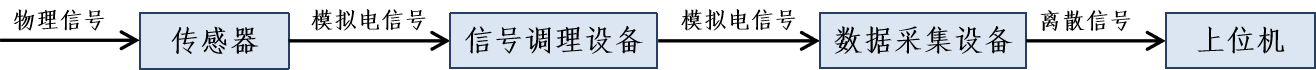
\includegraphics[scale=0.55]{2硬件设备流程图.png}
    \caption{\label{fig:framework}技术框架图}
\end{figure}
综合考虑成本和功能扩展性因素,在数据采集卡和上位机分析软件的结合方面,
本研究选用的方案是购买美国NI公司的数据采集卡,基于LabVIEW自行开发上位机软件。
通过LabVIEW调用硬件设备的底层驱动程序,结合软件功能模块,从而搭建出控制数据采集传输,处理和存储的系统。
该系统的的核心部分是功能模块的设计,本系统功能模块可分为系统设置模块、信号采集模块、数据显示模块、信号分析模块、数据管理模块等,
系统方案图如\autoref{fig:system}所示。此外还可以根据实际情况,灵活地添加新的功能模块。
在2.4节软件系统设计中将对软件模块的设计过程作详细介绍。
\begin{figure}[htbp]
    \centering
    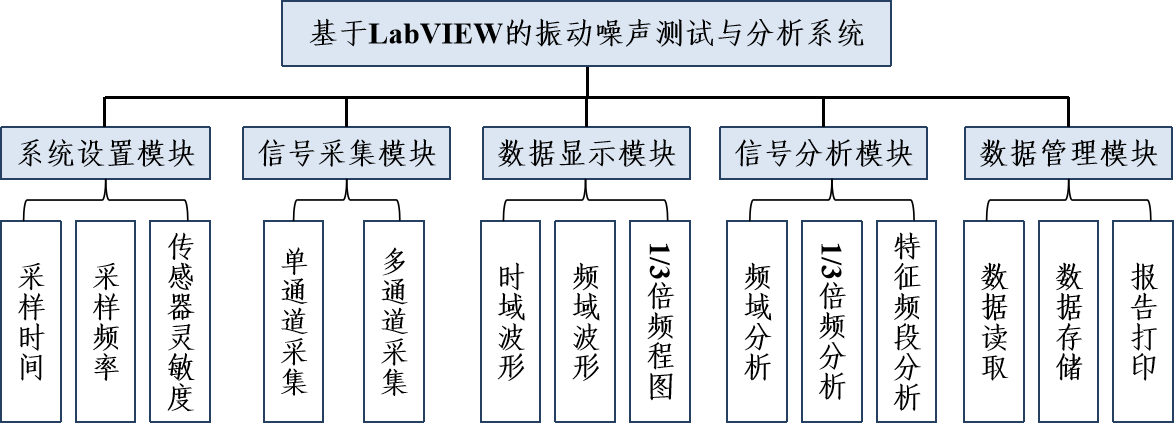
\includegraphics[scale=0.6]{2系统方案.png}
    \caption{\label{fig:system}系统方案图}
\end{figure}

\section{测试系统硬件设计}
针对本研究所涉及的测试场景,传感器需要支持远距离传输,简单电路调理等功能,
因此本研究选用了抗干扰能力强,内置放大器等要求的传感器类型。
传感器由于内置了专门的集成调理电路,属于有源传感器,而该电路要正常工作需要恒流源供电。
这样一来,一方面系统可以不用设置额外的信号调理设备,简化了测试系统。
另一方面对数据采集设备也提出了要求,主要包括以下几个方面,(1)支持多通道同步采集;
(2)支持IEPE信号调理;(3)轻巧灵活,便携式;(4)支持USB外设总线技术。

为满足本系统在实际试验中应具有的便携式特点,且在综合考虑了通道数、分辨率、量程、相对精
度、稳定时间和噪声等各方面因素的情况下,经过对比分析,
本研究选用了USB-​NI9231采集卡,如\autoref{fig:acquire}所示。
​NI9231是NI公司的一种8通道高速动态信号采集卡,兼容USB接口,AC/DC耦合方式可选,
可对IEPE传感器进行高精度测量。
NI9231带有2mA恒定电流的集成电路压电式(IEPE)信号调理,包含内置抗混叠滤波器,
可自动调节至设置的采样率,也对采集系统进行了接地屏蔽处理,
输入通道可同时以最高为51.2$\mathrm{kHz}$的速率对信号进行数字化。

\begin{figure}[htbp]
    \centering
    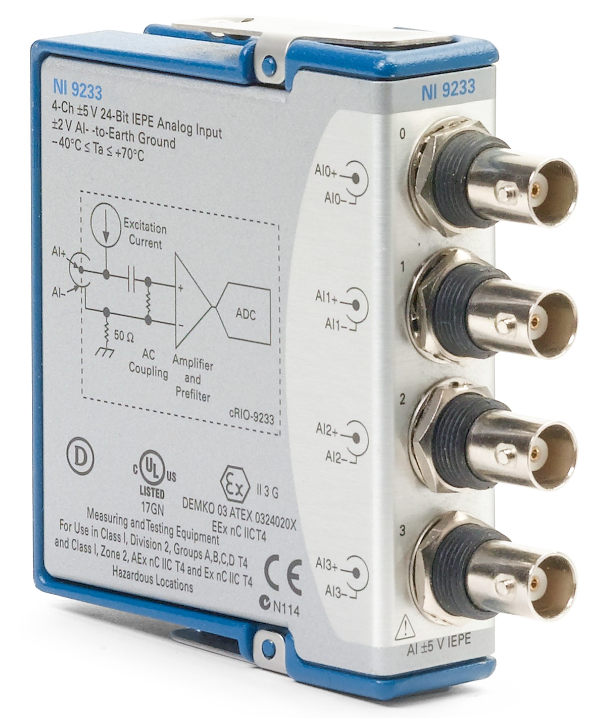
\includegraphics[scale=1]{2数据采集卡.png}
    \caption{\label{fig:acquire}数据采集卡}
\end{figure}
​
数据采集卡每个通道的输入信号经缓冲,放大器和预滤波器调理后,由模数转换器对其采样。
数据采集卡内部系统结构如\autoref{fig:acquire}所示。
数据采集卡采集数据时,数据传输方式包括直接内存访问(DMA),中断请求(IRQ)和可编程I/O。
IRQ传输方式会置高信号并中断处理器,然后由处理器处理数据传输。
IRQ 传输通常很低,只有150 kb/s。
DMA是一种DAQ板卡和PC内存间直接通讯的传输方式,不再需要处理器的干预。
NI内置芯片可以处理与PCI总线间的所有总线协议,DMA传输速率很高,可以高达20 Mb/s。
NI数据采集系统中默认是使用DMA传输方式。

数据采集卡的传输过程为,外部的信号进入数据采集卡后,经过各种处理转换,
先进入数据采集卡自身的缓冲区里面,缓冲区是先进先出(FIFO,First In First Out)的。
NI的数据采集卡有板载的缓冲区,不同数据采集卡的缓冲区的大小不一样,
板载缓冲区的大小一般是出厂商固定的,无法更改。
然后当板载缓冲区中的数据量到了一定的条件时,
数据采集卡将缓冲区的数据以DMA(直接内存访问)方式上传到计算机内存中,
\begin{figure}[htbp]
    \centering
    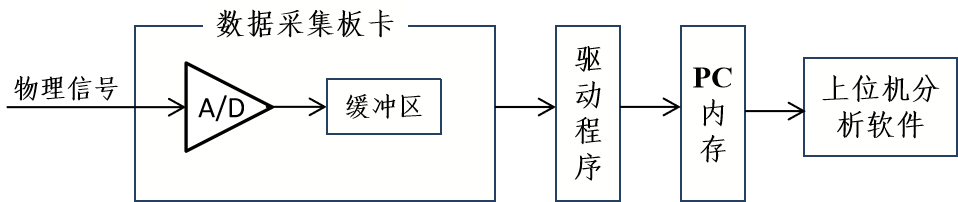
\includegraphics[scale=0.6]{2数据采集卡系统结构.png}
    \caption{\label{fig:acquire}数据采集卡系统结构}
\end{figure}

\section{测试系统软件设计}
在对软件系统进行设计之前,最先需要考虑的是计算机与硬件的交互。
和硬件交互需要两个基本要素:第一,硬件和计算机的通信接口和通信协议。
常用的接口及协议有USB 、LAN和PXI通信总线等等;
第二,交互命令,即通过上述通信接口按照协议发送的逻辑程控指令,例如仪器程控中常见的有VISA 、SCPI命令架构体系。

LabVIEW最大优势就是和测量硬件交互的便利性。
因为一方面NI公司将与硬件交互的逻辑指令按功能组织成硬件驱动(driver),可以直接下载安装。
另一方面NI的数据采集板卡一般都支持多种外设总线技术,比如PCI、USB,
外设总线的作用是允许外部IO设备与计算机CPU和内存通信。
使用LabVIEW连接硬件系统时,需要一个工具软件NI-MAX,即Measurement\&Automation Explorer(MAX),
用来验证驱动安装与否和连接的正常性检查。
在我们安装好驱动之后,用NI-MAX软件验证连接和驱动的工作正常性。
硬件调试好以后,就可以在LabVIEW中进行编程从而实现具体的业务功能。

LabVIEW是图形化的编程语言,编程方法不同于传统程序设计方法, 它摆脱了传统语言线性结构的困扰, 
执行顺序是由数据流的方式确定。
本研究基于LabVIEW面向过程的编程思想,使用了通知器、队列和事件的设计模式,
实现了系统设置模块、信号采集模块、数据显示模块、信号分析模块、数据管理模块等模块的设计。
软件的主界面如\autoref{fig:main}所示,各功能模块集成到该主界面上。
\begin{figure}[htbp]
    \centering
    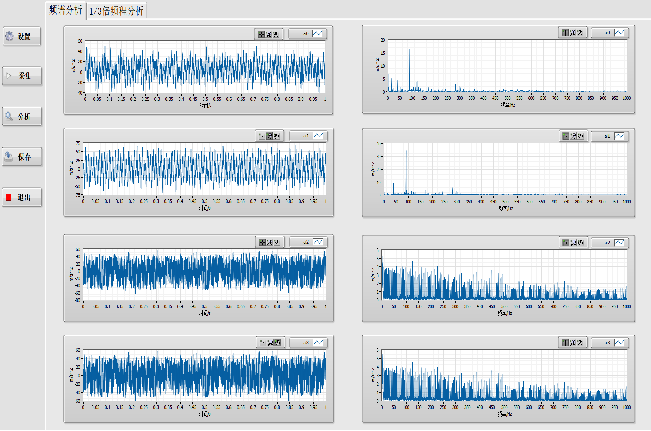
\includegraphics[scale=0.25]{2软件主界面.png}
    \caption{\label{fig:main}软件主界面}
\end{figure}

推进泵噪声测试系统测量流程是:首先等待各部分参数设置好后,发出采集启动信号,
同步采集各通道数据,采集完成后数据自动存储在相应文件中。信号分析会从文件中读取数据,
分析结果实时展示在界面。程序设计流程如\autoref{fig:process}所示。
\begin{figure}[htbp]
    \centering
    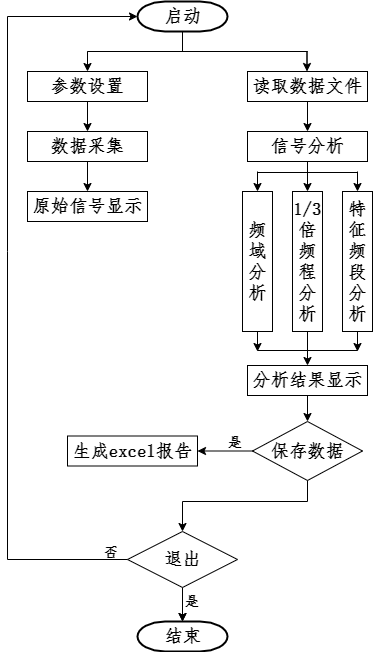
\includegraphics[scale=0.55]{2软件流程图.png}
    \caption{\label{fig:process}程序流程图}
\end{figure}

\begin{comment}
\subsection{系统设置模块}
软件界面的设置模块提供了测试系统各项参数设定,包括采集通道设置、采样参数设置、
传感器灵敏度设置、分析参数设置等。
\begin{figure}[htbp]
    \centering
    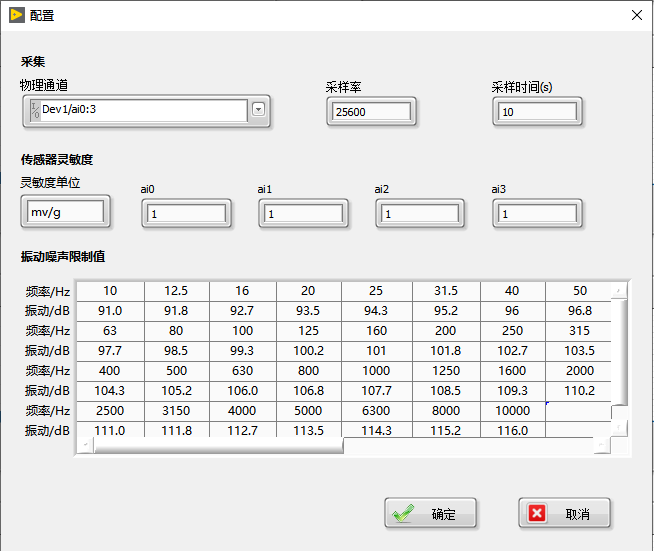
\includegraphics[scale=0.55]{2系统设置.png}
    \caption{\label{fig:setting}系统设置}
\end{figure}
\end{comment}

\subsection{数据采集模块}
在对数据采集模块进行设计时,本研究主要考虑如下几个方面:(1)如何保证数据在采集过程中不丢失?
(2)实现采集数据的实时存储。
在2.3节提到程序最终是从计算机内存读取数据,而这个缓存区的大小是我们可以指定的。
缓冲区存储数据量的大小又是和它的输入速度和输出速度有关,输入速率是由采样率所决定的,
输出速度就是采集程序从它里面读取的速度。
假如计算机内存缓冲区设置的过小,或者输出速率过慢,都有可能导致缓存区的溢出,出现数据丢失的情况。
计算机内存缓冲区设置的过大,在硬盘和内存之间会产生过量的读写操作,也会对系统性能造成影响。

所以为了保证数据不会丢失,要设置好内存缓冲区的大小,
还要保证读取缓冲区的程序(DAQmx Read.vi)循环得尽量快,每一次读取的数据尽量多。
LabVIEW中缓冲区大小的设置也和采样模式有关,常用的采样模式为有限采样和连续采样,本研究采用连续采样模式。
对于连续采样模式,NI-DAQmx设置的缓存区大小如\autoref{tab:sample}所示,缓存区大小建议是采样率的10倍左右。
对于读取缓冲区的程序(DAQmx Read.vi)来说,设置成多采样,每次都是将内存中的所有数据读取进来,就能实现读取的数据尽量多。
\begin{table}[htbp]
    \centering
    \caption{\label{tab:sample}NI-DAQmx连续采样缓存区大小}
    \begin{tabular}{ccc}
     \toprule
     采样率&缓冲区大小\\
     \midrule
     未指定速率&10 kS\\
     0-100 S/s&1 kS\\
     100-10,000 S/s&10 kS\\
     10,000-1,000,000 S/s&100 kS\\
     >1,000,000 S/s&1 MS\\
     \bottomrule
    \end{tabular}
\end{table}

为实现数据的实时存储,本研究采用了生产者/消费者的模式,
生产者/消费者结构基于队列的数据结构,即开辟一个缓存区,依据先进先出的原则进行\cite{马瑾2015基于}。
新来的元素总是被加入队尾,每次离开的元素总是从队首离开。程序中新采集的数据加入到
队尾,队首出队的元素同步保存在相应文件中。
这样就保证了数据存储过程中不会出现数据丢失的现象,能实现实时存储。
数据采集程序框图如\autoref{fig:soft}所示。
\begin{figure}[htbp]
    \centering
    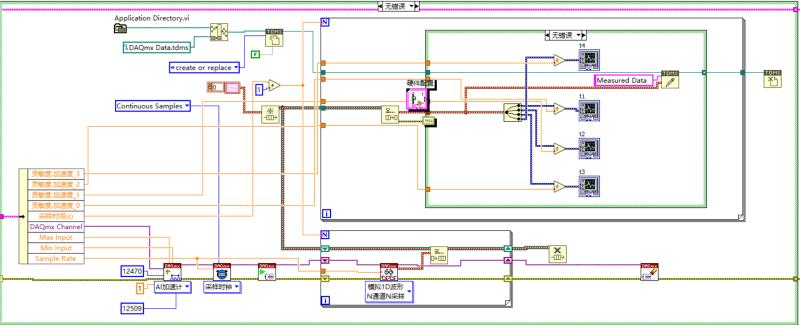
\includegraphics[scale=0.85]{2数据采集程序框图.jpg}
    \caption{\label{fig:soft}数据采集程序框图}
\end{figure}


\subsection{信号分析模块}
LabVIEW适合于数据采集、仪器控制、和图像显示等应用,可以高效地构建虚拟仪器系统。
然而这种图形化的软件开发环境对于复杂的数值计算和分析要求就显得力不从心。
在对各种信号分析算法的支持方面,LabVIEW的工具箱也非常有限。
LabVIEW8.2以后版本推出了仿真框图和面向数学的文本编辑语言MathScript,它带
有交互式窗口和可编辑的接口,通过MathScript用户可以在LabVIEW图形化程序中运行较简单的m文件语法脚本\cite{周惠2007LabVIEW,柴敬安2008Labview}。
因此LabVIEW提供了与MATLAB进行通信的方式,本研究借助数据处理能力更强的MATLAB进行信号的分析。

MATLAB也支持ActiveX自动化技术,LabVIEW程序在运行MATLAB Script节点时,会启动一个MATLAB进程执行脚本的内容,
并且与MATLAB的工作空间进行数据交换。但是MATLAB Script节点对输入、输出数据的类型有明确的要求,只有
LabVIEW中的数据类型与MATLAB中的数据类型相匹配,才能够进行数据交换\cite{苏宝定2008基于}。
将采集模块中获取的数据导入如\autoref{fig:otc}所示的节点中,便可获得信号频谱分析和1/3倍频程分析的结果。
\begin{figure}[htbp]
    \centering
    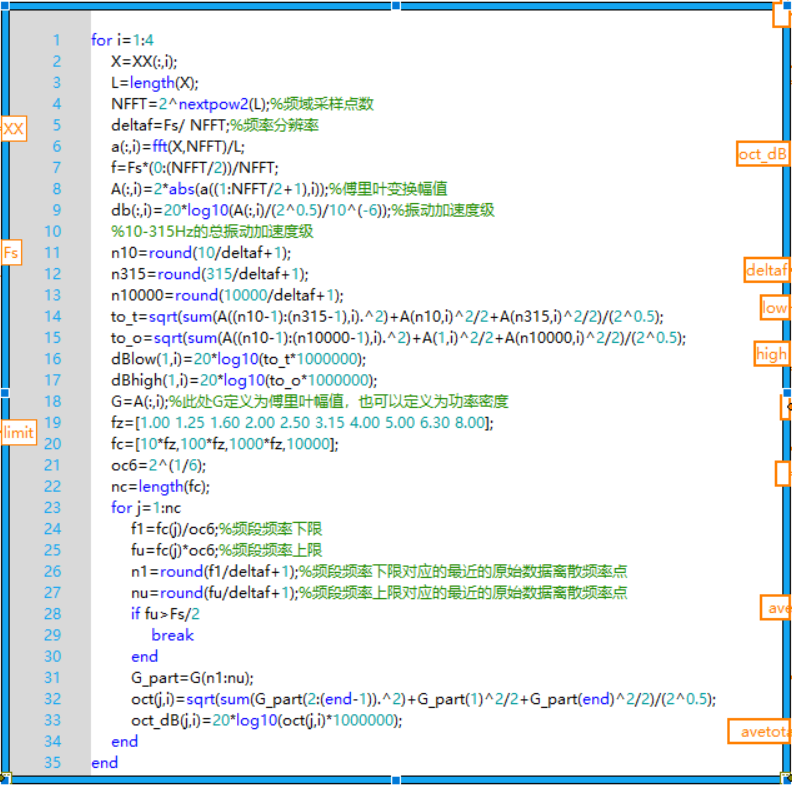
\includegraphics[scale=0.75]{2倍频程程序.png}
    \caption{\label{fig:otc}mathscript节点部分进行1/3倍频程分析的程序}
\end{figure}

软件分析模块的展示界面如\autoref{fig:analyze}所示,包含了各通道信号的频谱图、
三分之一倍频程图,以及三分之一倍频程和特征频段总声压级的表格展示。
\begin{figure}[htbp]
    \centering
    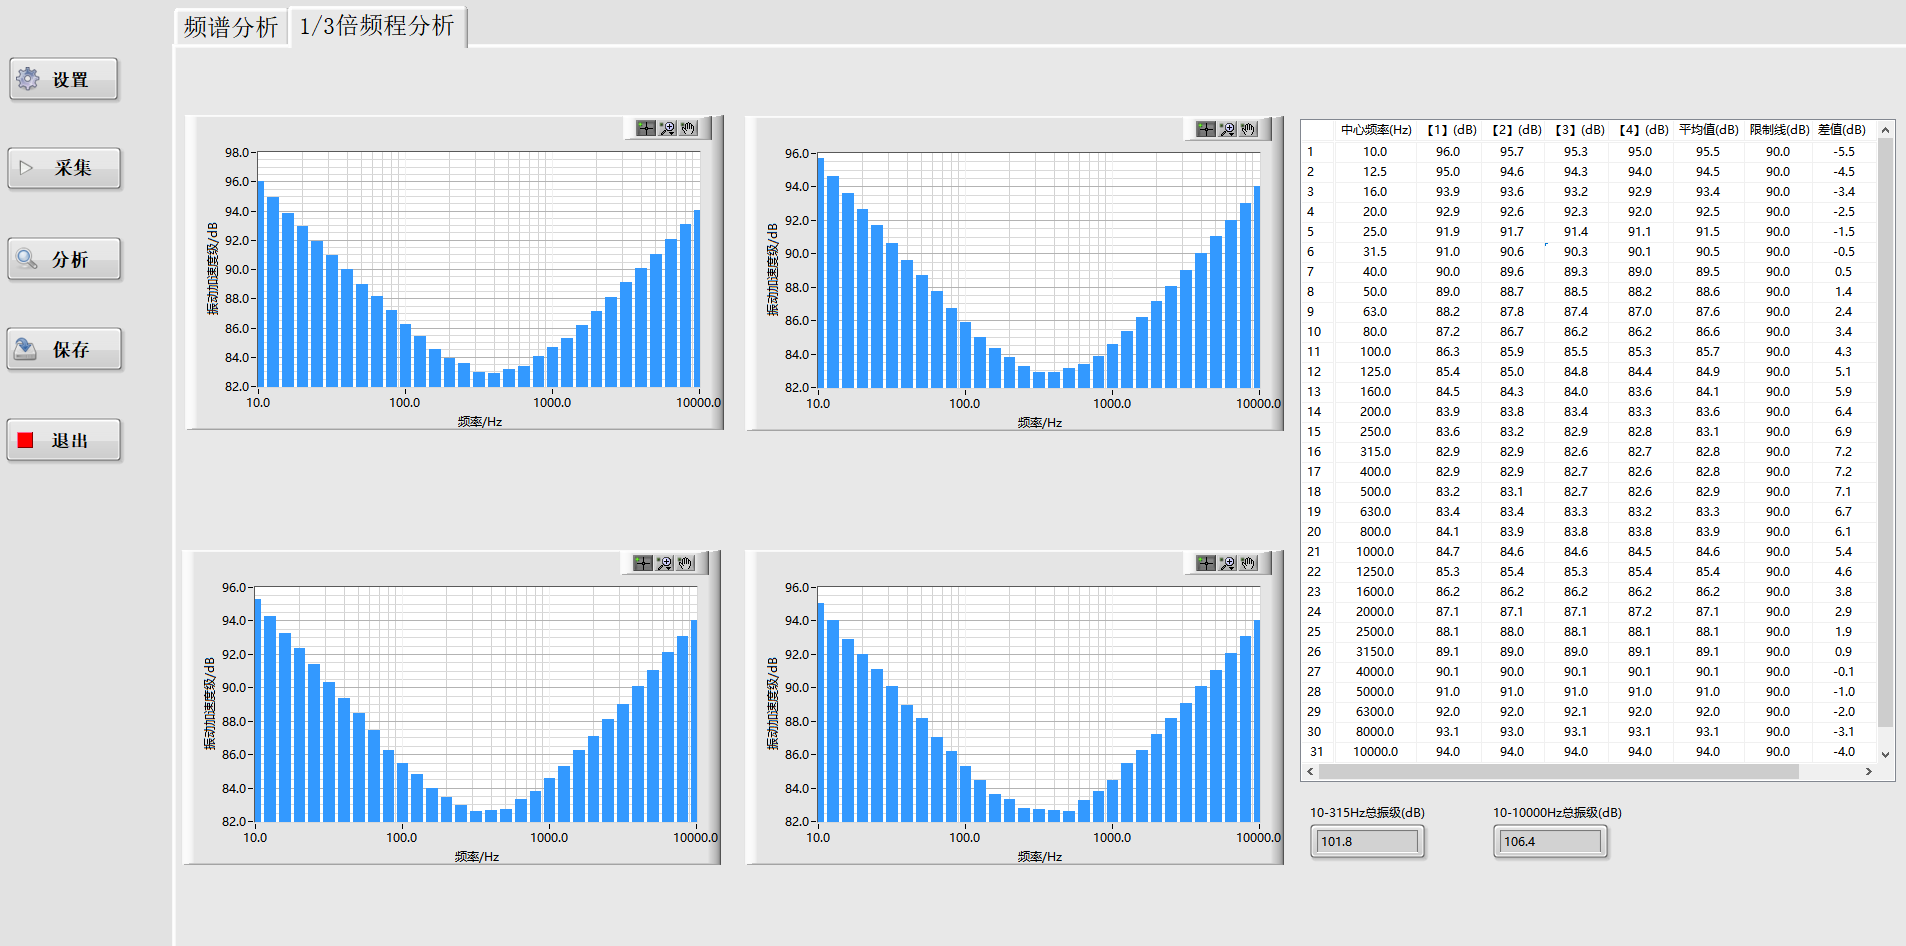
\includegraphics[scale=0.25]{2软件分析模块.png}
    \caption{\label{fig:analyze}系统信号分析界面}
\end{figure}

\subsection{数据管理模块}
数据管理模块包含采集数据的实时存储、采集数据的读取和分析数据的存储。
由于实验是多通道数据采集,且采样速度要求较高,因此数据量较大。为了方便实时存储和
管理这些数据,程序采用TDMS文件格式。TDMS文件格式是NI主推的一种二进制记录文件,
它兼顾了高速、易存取和方便等多种优势,在记录的仿真或测量数据的同时,也会存储描述性信息,
包括测试过程,传感器信息等,数据实时存储程序框图如\autoref{fig:save}所示。当数据采集完成进行分析时,程序会从已保存的TDMS文件中读取数据
导入分析模块进行,数据读取程序框图如\autoref{fig:read}所示。

分析完成数据将会以excel表格的形式进行存储。
主程序中从VISAread的readbuffer端读上来的数据需要转换成表格数据进行保存,
数据的保存分为两个阶段。第一阶段,通过表单形式显示在主程序界面,
方便用户直观查看测试参数是否已满足要求。
第二阶段,用户可选择把表单数据保存到Excel文件中,以供用户保存和打印。
\begin{figure}[htbp]
    \centering
    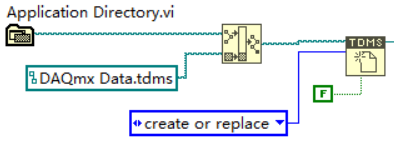
\includegraphics[scale=0.85]{2文件存储.png}
    \caption{\label{fig:save}数据实时存储程序框图}
\end{figure}
\begin{figure}[htbp]
    \centering
    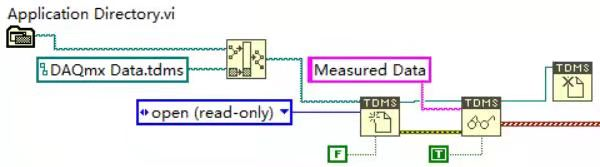
\includegraphics[scale=0.45]{2文件读取.jpg}
    \caption{\label{fig:read}数据读取程序框图}
\end{figure}
%\section{性能测试}
\section{本章小结}
本章基于LabVIEW设计了推进泵噪声测试与分析系统,
针对系统的硬件设计、软件设计进行了阐述说明,主要完成了以下工作:

(1)对推进泵噪声试验平台和测试基本参数,以及声纹特征的分析需求进行了详细分析阐述,
制定了噪声测试与分析系统的技术框架和系统方案。

(2)阐述了系统的硬件组成、传感器型号及参数,研究了数据采集卡的系统结构和传输过程,
对硬件与计算机的交互通信进行了说明;

(3)完成了软件系统的各个功能模块的设计。阐述了软件操作流程,
实现了软件上位机系统程序框图及界面设计,对信号采集模块、信号分析模块、数据管理模块等模块的程序框图进行了详细说明。

推进泵噪声测试与分析系统为开展推进泵噪声的试验研究奠定了研究基础,可提高测试和分析任务的运行效率,
具有操作简单,经济高效等优势。
该系统不仅适用于推进泵振动及噪声测试场景,
也可以推广到离心泵、风机等动设备振动与噪声测试场景中使用。
至此完成了推进泵噪声测试与分析系统的硬件设计、软件设计等工作,接下来将进行推进泵噪声试验及试验数据分析。

\chapter{推进泵噪声的声纹特征分析}\label{ch:chapter3}
\section{引言}
本文以紧凑型前置导叶的单级推进泵和新型结构的双级推进泵为研究对象,
在大型空泡水洞中对其进行噪声试验研究。
目的在于阐明推进泵辐射噪声特性与航速之间的声学关联性,以及丰富推进泵声指纹特征的内涵。

试验中通过固定叶轮转速、改变水洞流速的方法,从而获得推进泵在不同水动力性能工况下的噪声数据。
由于水洞测试的局限性会影响推进泵中低频段辐射噪声的声压级量级,所测噪声信号的信噪比较低。
因此在研究中对多工况下的水洞背景噪声
进行了试验测量,分析了水洞背景噪声的频谱特性和特征频段能量分布,
讨论背景噪声对推进泵噪声的影响;其次,采集了单级推进泵和双级推进泵在不
同水动力性能工况下的噪声数据,基于噪声采集与分析系统的分析模块,借助频谱分析
和三分之一倍频程分析等信号分析手段对推进泵噪声数据进行处理。在考虑背景噪声影
响的基础上,研究不同工况下推进泵噪声的声纹特征变化,以及流速等与噪声的声学关
联性,探讨推进泵噪声的声纹特征。
\section{水洞背景噪声的试验研究}
借助空泡水洞对推进泵辐射噪声进行测量时,是用有限场来探索无限场噪声,会影响声压测量的可靠性。
根据国际船模水池会议(ITTC)的建议,在空泡水洞中进行噪声声压测量时必须满足声模数准则\cite{曾赛2018试验研究}。
\begin{equation}
    \label{equ:fm}
    N=\frac{\pi f^3V}{c^3} > 1
\end{equation}

式中,$N$为声摸数,$c$为水中声速,$f$为噪声频率,$V$为试验段体积。将试验空泡水洞参数代入计算,
可知测得的推进泵辐射噪声声压级比较可靠的频段是大于1 kHz的频段。
同时由于水舱中存在壁面反射等效应,对推进泵噪声,尤其是中低频噪声影响较大。
这些因素会导致所测量的噪声信号的信噪较低,从而影响推进泵中低频段线谱和宽带谱噪声的声压级量级。
因此,本章主要讨论噪声信号声压级在不同工况下的相对量级,重点关注不同工况下推进泵噪声的声纹特征变化,
从而探讨流速与推进泵噪声的声学关联性。

此外,在对推进泵噪声进行试验之前,本研究中测量了水洞在未安装推进泵状态的背景噪声。将水速从1.02 m/s增加至5.59 m/s,
对该范围内的20个工况点进行了背景噪声的测量。目的在于研究背景噪声的声纹特征,
分析背景噪声对推进泵噪声的影响。
%因此在本文仅讨论水速对噪声各频段的影响,以及各频段噪声对噪声总声压级的贡献度。
\begin{figure}[htbp]
    \centering
    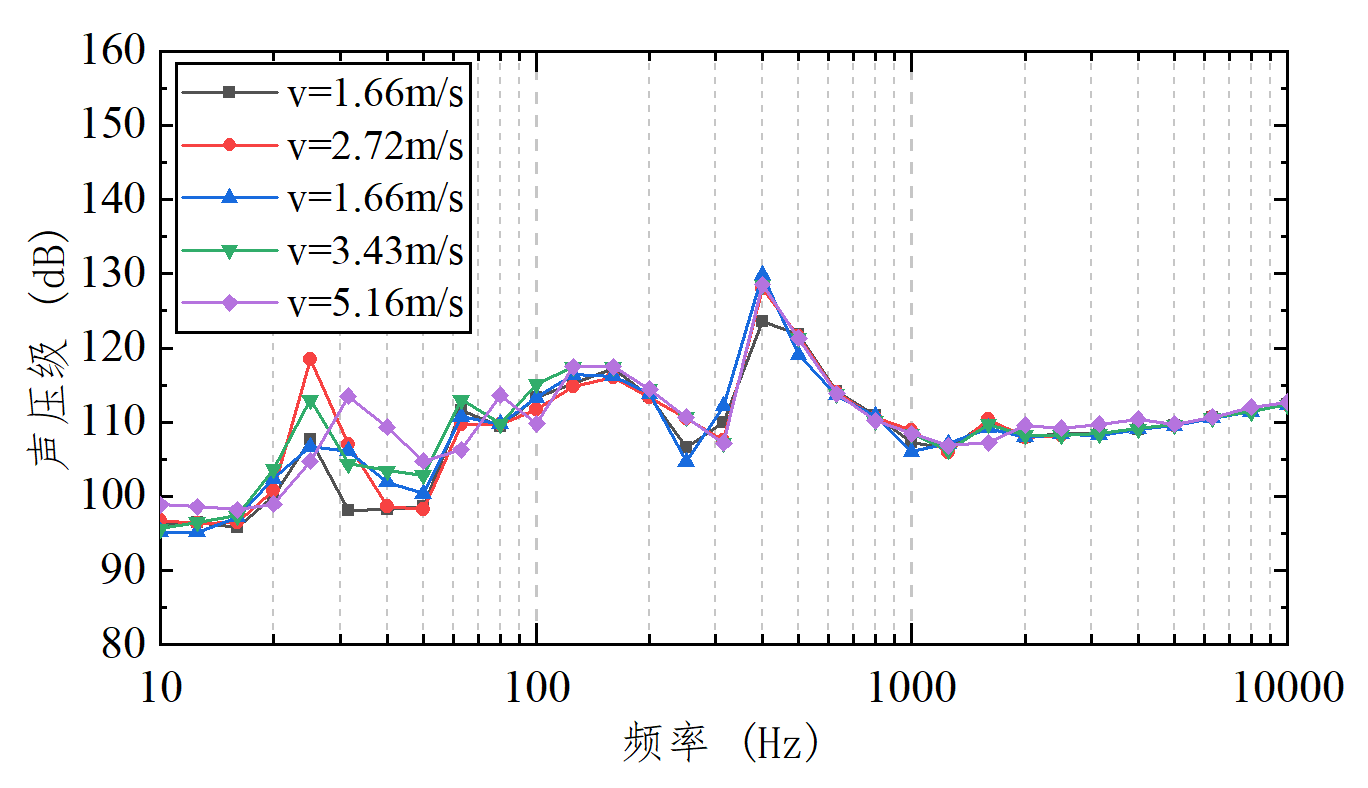
\includegraphics[scale=1]{3背景噪声的倍频程图.png}
    \caption{\label{fig:otcbeijing}水洞背景噪声1/3倍频程分析}
\end{figure}

如\autoref{fig:otcbeijing}所示为水洞不同流速下的背景噪声1/3倍频程图,
可表征频域能量分布。
可以看出水洞背景噪声能量在中低频段分布上有明显波动。
高频段能量分布曲线平坦,单位频域下分布几近相同的能量密度。
随着水速的增大,背景噪声各频段上的能量分布变化不大。

\begin{figure}[htbp]
    \centering
    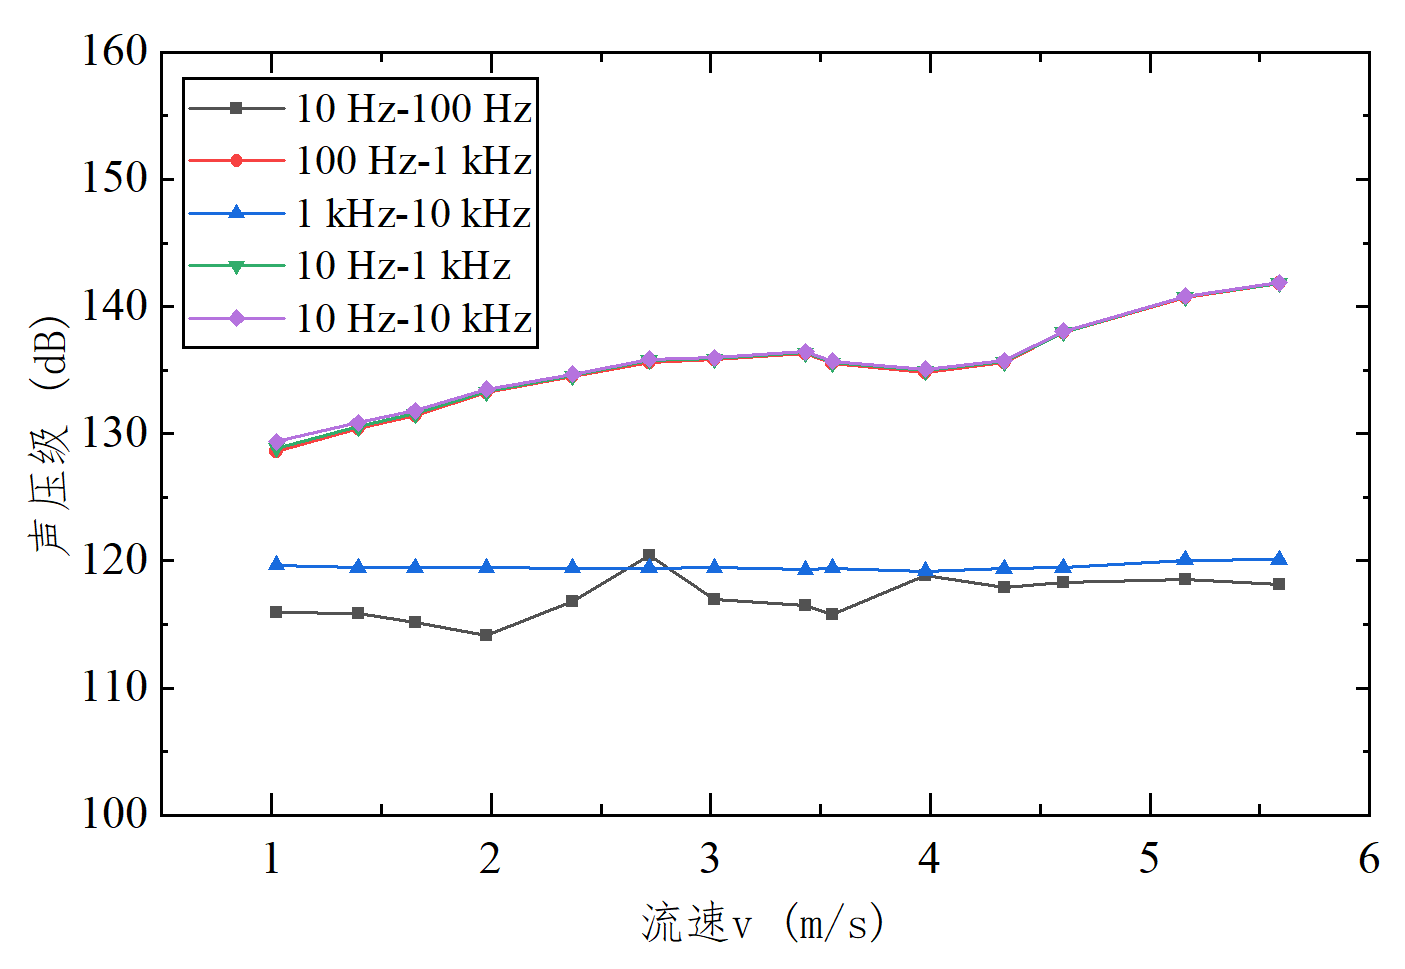
\includegraphics[scale=1]{3背景总声压级1.png}
    \caption{\label{fig:beijingtotal}水洞背景噪声在不同水速下各个频段的噪声总声压级}
\end{figure}

如\autoref{fig:beijingtotal}所示为水洞背景噪声在不同流速下各个频段的总声压级。
从图中可以看出,随着流速的提升,高频段(1kHz -10 kHz)的声压级几乎没有发生变化。
而低频段(10Hz -1 kHz)的总声压曲线随着流速的变化来回波动,没有明显的变化规律,
但是总体来看低频段的声压级没有出现随流速增大而增大的趋势。
中频段(100Hz-1kHz)、中低频段(10Hz-1kHz)和全频段(10 Hz-10kHz)的变化曲线几乎重合,并且曲线随流速增大单调递增。
这说明中频段(100Hz-1kHz)噪声是背景噪声最主要的贡献量,流速的增大会提升中频段(100Hz-1kHz)的噪声能量,
进而增强背景噪声的总能量。

如\autoref{fig:beijingfft}所示为水洞在水速为4.5m/s工况下的背景噪声频谱图,
频谱在中低频段有连续的线谱成分,线谱幅值量级明显高于宽带谱,从而造成中低频段的能量波动。
其中100Hz和300Hz线谱最为突出,为电磁干扰频率。结合三分之一倍频程图,可以看出电磁干扰频率及其附近频率成分影响了频谱的能量分布。

\begin{figure}[htbp]
    \centering
    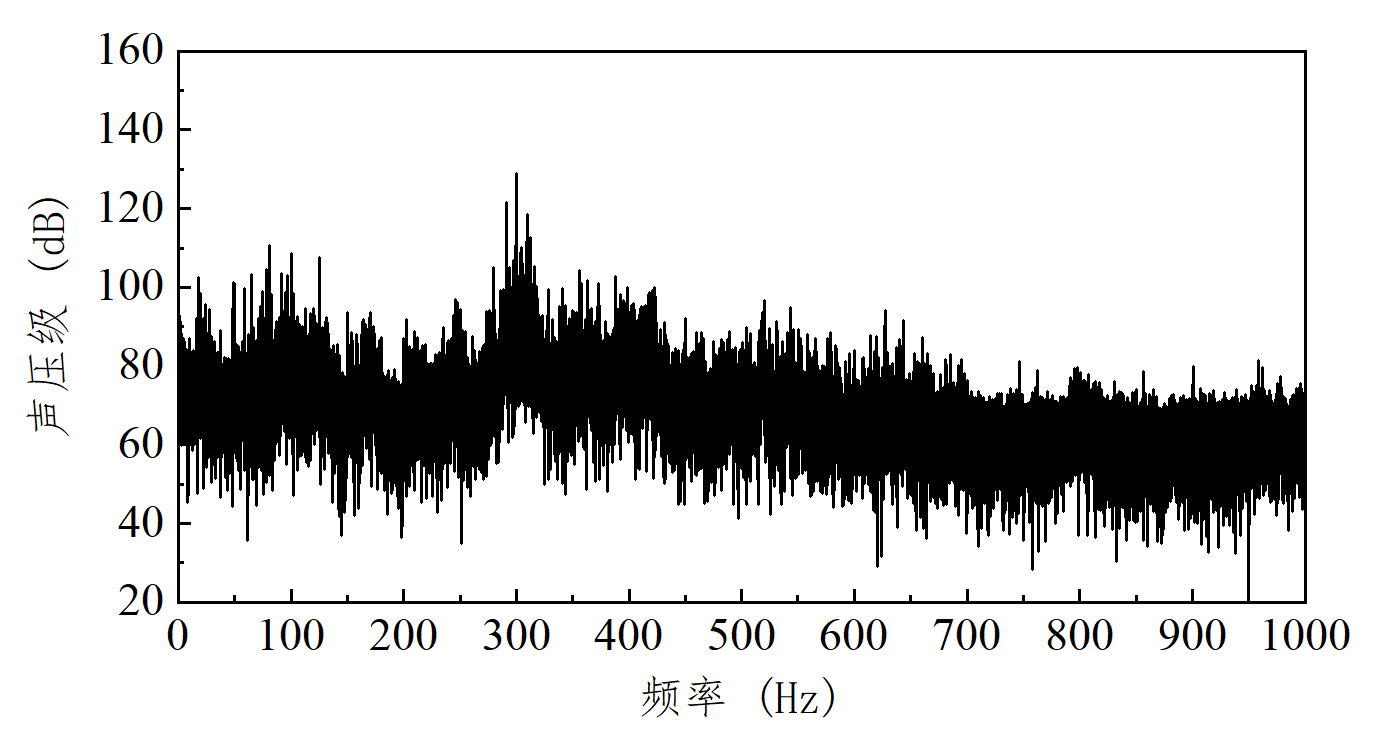
\includegraphics[scale=1]{3背景噪声频谱.png}
    \caption{\label{fig:beijingfft}v=4.5m/s工况下水洞背景噪声频谱}
\end{figure}

以上分析表明,背景噪声的频谱呈现出中低频段宽带和线谱交叠的形貌,其中100Hz和300Hz电磁干扰线谱成分显著突出。
背景噪声的能量主要集中在中低频段,中低频段的线谱是背景噪声能量的主要贡献者。
背景噪声对推进泵噪声的影响将主要体现在中低频段(10Hz-1 kHz),会降低推进泵中低频段噪声的信噪比。
因此在后文对推进泵噪声的分析中将会参考水洞背景噪声的频谱特性和
特征频段能量分布,探究流速与推进泵噪声各频段的声学关联性,
关注不同工况下推进泵噪声的声纹特征变化。
\section{单级推进泵声纹特征的试验研究}
\subsection{推进泵试验模型}
本小节的研究对象是一种紧凑型前置导叶推进泵,
其设计参数根据某航行体的推进需求计算,并进行缩尺得到。
最终确定轮缘直径200mm,并采用11片导叶加7片叶片的形式。
导管的设计选用33号减速喷管,可在一定程度上降低入流速度充分提升叶轮的抗空化性能,
并根据动量定理确定导管得出口直径,保证推进器能产生足够的推力。
导叶设计的核心问题就是如何设置合理的预旋,来达到更高的效率,
导叶的作用方式如\autoref{fig:daoye}所示。
\begin{figure}[htbp]
    \centering
    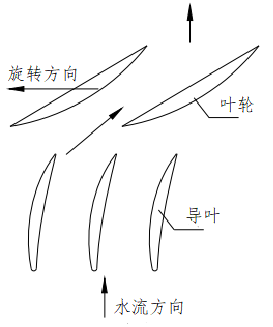
\includegraphics[scale=1.0]{3导叶作用方式.png}
    \caption{\label{fig:daoye}导叶作用方式}
\end{figure}
叶轮的设计主要考虑了以下几个方面:(1)将定转子间距增大为0.2倍轮缘直径来减小定转子之间干涉;
(2)通过缩短叶顶长度进一步减小叶轮顶部的载荷,来减小叶顶泄漏带来的效率损失,提升推进器总体能效水平;
(3)将叶轮剖面翼型的最大厚度后移到40\%弦长处,优化吸力面压力分布,延迟空化的发生。
推进泵设计模型如\autoref{fig:dj_design}所示。
\begin{figure}[htbp]
    \centering
    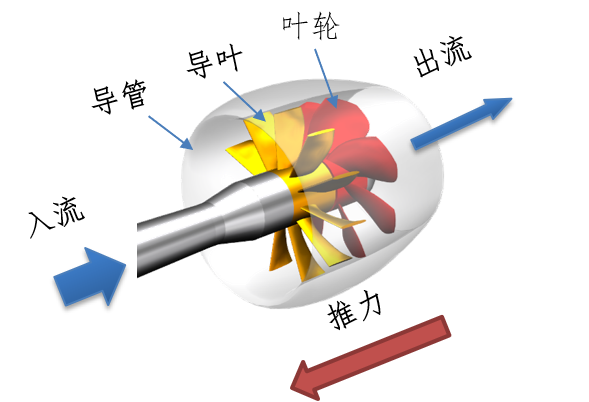
\includegraphics[scale=1.0]{3单级整体结构.png}
    \caption{\label{fig:dj_design}单级推进泵设计模型}
\end{figure}

推进泵的设计参数如\autoref{tab:dj}所示。
\begin{table}[htbp]
    \centering
    \caption{\label{tab:dj}单级推进泵设计参数}
    \begin{tabular}{ccc}
     \toprule
     参数&值\\
     \midrule
     D(叶轮直径,mm)&200\\
     N(设计转速,rpm)&1260\\
     L(导管长度,mm)&240\\
     $D_1$(入口直径,mm)&228\\
     $D_2$(出口直径,mm)&182\\
     $Z_1$(叶轮叶片数)&7\\
     $Z_2$(导叶叶片数)&11\\
     轮毂比&0.3\\
     旋向&右旋\\
     %APF(轴频,Hz)&21\\
     %BPF(叶轮叶频,Hz)&147\\
     %SBPF(导叶叶频,Hz)&231\\
     \bottomrule
    \end{tabular}
\end{table}
推进泵试验模型的叶轮采用铝合金加工制造,表面做阳极化处理。导管选用有机玻璃材质,便于观察其特性。
单级推进泵试验模型如\autoref{fig:dj_test}所示。
\begin{figure}[htbp]
    \centering
    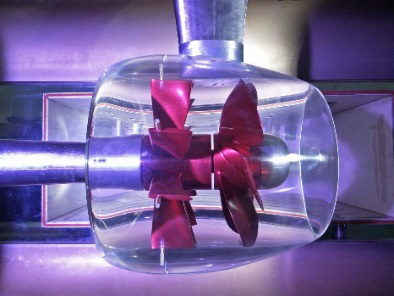
\includegraphics[scale=2]{3单级试验模型.png}
    \caption{\label{fig:dj_test}单级推进泵试验模型}
\end{figure}
为了获得推进泵在不同水动力工况下的噪声数据,
试验中通过固定叶轮转速、改变水洞流速的方法测量了不同进速系数工况点下的单级推进泵
水动力性能和噪声数据。

在推进泵水动力性能试验方面,结合主轴扭矩与转速等数据计算推进泵叶轮的功率、扬程、水力效率,
借助动力仪测量多工况下推进泵的推力性能,可得到推进器的敞水性能曲线。
空泡水筒测力系统可以独立测量旋转部件和静止部件产生的推力,
由天平测量得到导管和导叶(包括连接机翼阻力)的总推力$T_{D}$。
导管和导叶推力为天平测得的总推力减去导管连接机翼阻力$(F)$,
即$T_{D}=T_{D}-F$。在均匀流场常压条件下,推进器模型敞水性能试验采用定转速,
改变来流速度以获得相应于各个进速系数$J$的推力系数,扭矩系数$K_{Q}$等水动力数据。
推力系数、扭矩系数等定义如\autoref{equ:three1}至\autoref{equ:three7}所示。
\begin{equation}
    \label{equ:three1}
    J=\frac{V}{nD} 
\end{equation}
\begin{equation}
    \label{equ:three2}
    Re =\frac{C_{0.7R}\sqrt{V^{2}+\left ( 0.7\pi nD \right )^{2}   }  }{\upsilon } 
\end{equation}
\begin{equation}
    \label{equ:three3}
    K_{T}=\frac{T}{\rho n^{2}D^{4}  }  
\end{equation}
\begin{equation}
    \label{equ:three4}
    K_{TP}=\frac{T_{P} }{\rho n^{2}D^{4}  }  
\end{equation}
\begin{equation}
    \label{equ:three5}
    K_{TD}=\frac{T_{D} }{\rho n^{2}D^{4}  }  
\end{equation}
\begin{equation}
    \label{equ:three6}
    K_{Q}=\frac{Q}{\rho n^{2}D^{4}  }  
\end{equation}
\begin{equation}
    \label{equ:three7}
    \eta _{0} =\frac{J}{2\pi } \cdot \frac{K_{T} }{K_{Q}} 
\end{equation}

式中$D$表示叶轮直径$(m)$,$V$表示来流速度$(m/s)$,$n$表示转速$(r/s)$,
$Re$表示雷诺数,$C_{0.7}$表示叶轮0.7R处的弦长$(m)$,
$T$表示推进泵总推力$(N)$,$T_{P}$表示动叶推力$(N)$,
$T_{D} $表示导管加支架推力$(N)$,
$F$表示导管测力连接机翼阻力$(N)$,
$Q$表示扭矩$(N \cdot m)$,$K_{T}$表示推力系数,$K_{TP}$表示动叶推力系数,
$K_{TD}$表示导管支架推力系数,$K_{Q}$表示扭矩系数,
$\eta _{0}$表示效率。

将水洞试验测得的单级推进泵推力、转矩和效率等数据无量纲化后,得到如\autoref{fig:chanshuiquxian}所
示的敞水性能曲线。从图中可以看出:随着进速系数J的增大,
推力系数$K_T$和转矩系数$K_Q$逐渐减小,而推进效率$\eta_0$先增大后减小,
并在 J=1.0 处有最大值 61.2\%。与常见的螺旋桨敞水性能
曲线相比,单级推进泵的敞水性能曲线随进速系数增加时变化趋势平缓,具有较高推进
效率的同时也有较宽的高效工作区。
\begin{figure}[htbp]
    \centering
    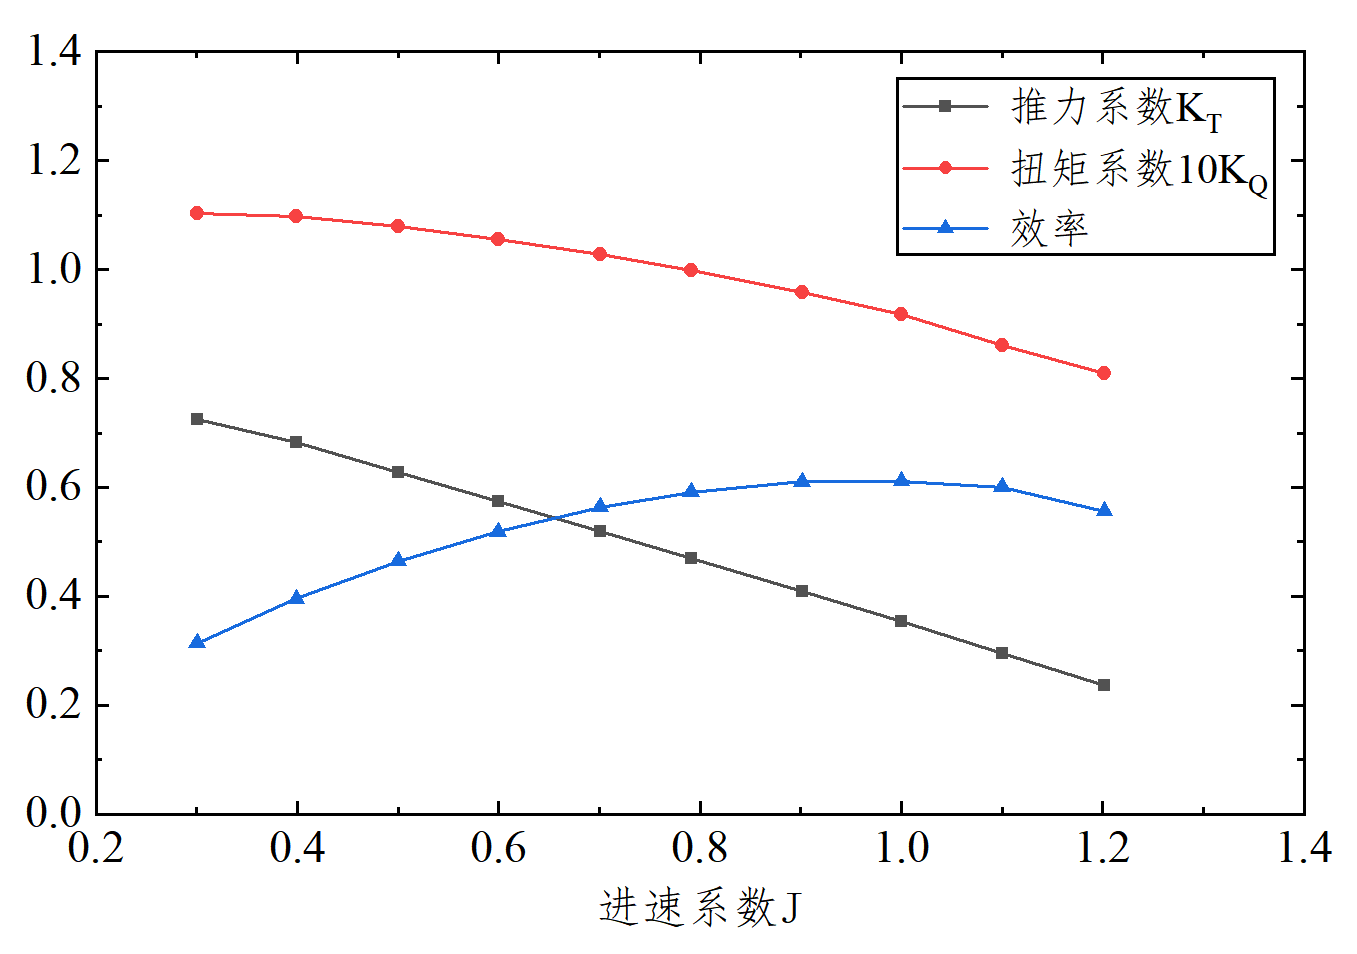
\includegraphics[scale=1]{3单级性能试验.png}
    \caption{\label{fig:chanshuiquxian}单级推进泵敞水性能曲线}
\end{figure}

本实验中利用水听器阵列进行推进泵辐射噪声的采集,其固定实验装置如\autoref{fig:djstq}所
示,加工好的木板在水舱中与水洞侧壁面平行放置,水听器垂直置于木板孔中,
图上标号表示水听器的安放位置。
利用水听器的空间位置布置,能够有效的进行推进泵在不同位置上的噪声采集。基于噪声测试系统
对上述位置的噪声信号进行同步采集,采样频率为20480Hz,每次测试采样时间为10s。
\begin{figure}[htbp]
    \centering
    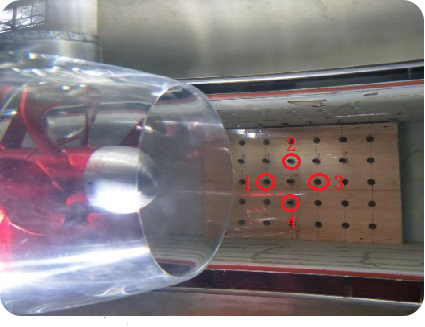
\includegraphics[scale=1.0]{3单级水听器布置.png}
    \caption{\label{fig:djstq}单级推进泵噪声试验中水听器布置}
\end{figure}
\subsection{推进泵噪声特性分析}
试验中通过固定叶轮转速为21rps,改变水洞流速的方法测量了进速系数0.3至1.2范围内10个工况点下的
水动力性能和噪声数据。
本文选取进速系数分别为0.4,0.6,0.79,1.0和1.2,
对应水速分别为1.68 m/s,2.52 m/s,3.32 m/s,4.2 m/s和5.05 m/s工况下的噪声数据进行分析。
基于噪声测试系统中的数据分析模块,获得了推进泵噪声的三分之一倍频程和频谱分析结果。

为了更好的表述推进泵噪声频谱的特性,本文对推进泵噪声频率的划分参考螺旋桨噪声的频率范围划分。
螺旋桨噪声频率范围的划分目前还没有统一的标准,其中
低频噪声通常在100 Hz以下,也有一些研究将其
范围取为200-500 Hz以下,高频噪声通常在1 kHz以上,而低频与高频之间过渡频
段的噪声也称为中频噪声\cite{xuye2019a}。
本文将推进泵低频噪声的频率范围划分为100 Hz以下,高频噪声在1 kHz以上,低频与高频之间过渡频
段的噪声划分为中频噪声。
\subsubsection{单级推进泵噪声三分之一倍频程分析}
\begin{figure}[htbp]
    \centering
    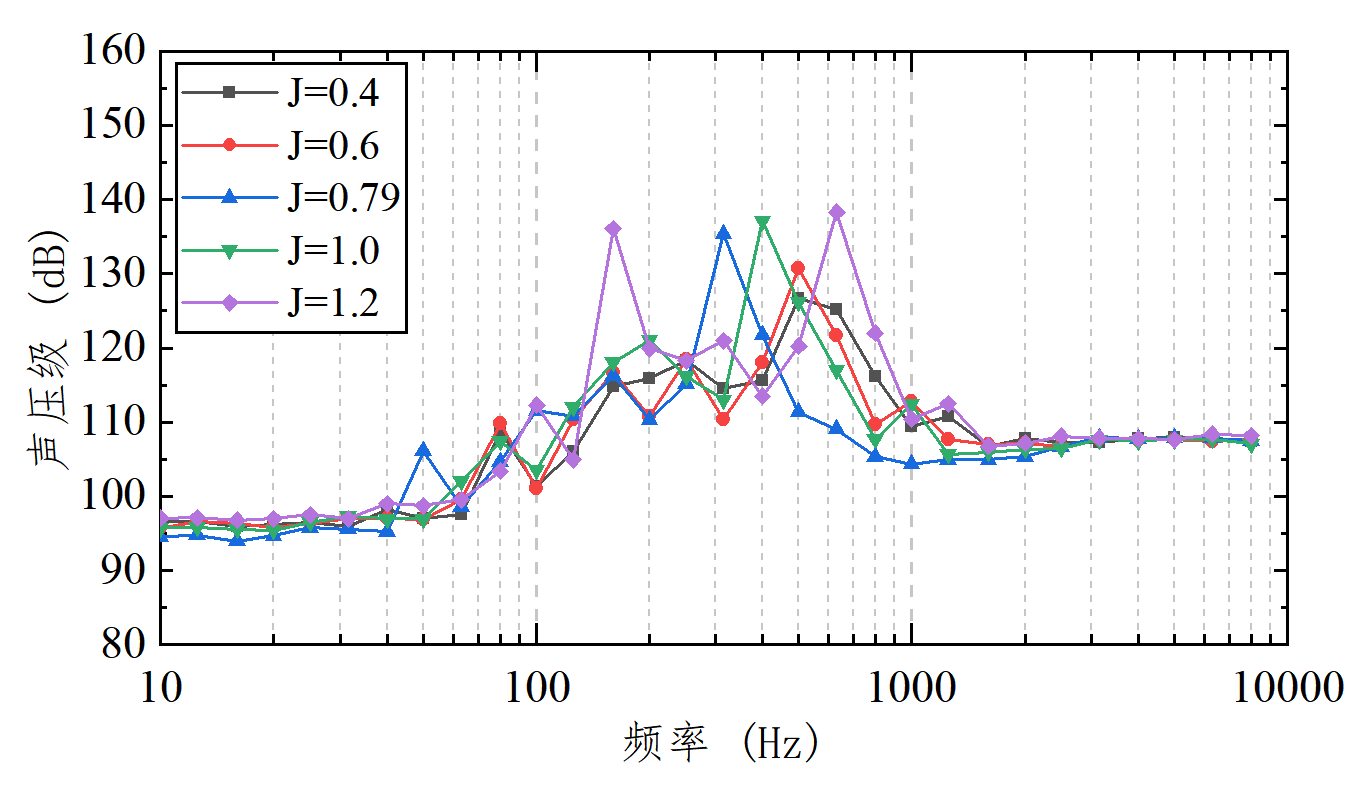
\includegraphics[scale=0.95]{3dj2_otc1.png}
    \caption{\label{fig:djotc1}单级推进泵噪声1/3倍频程分析(1号传感器)}
\end{figure}
\begin{figure}[htbp]
    \centering
    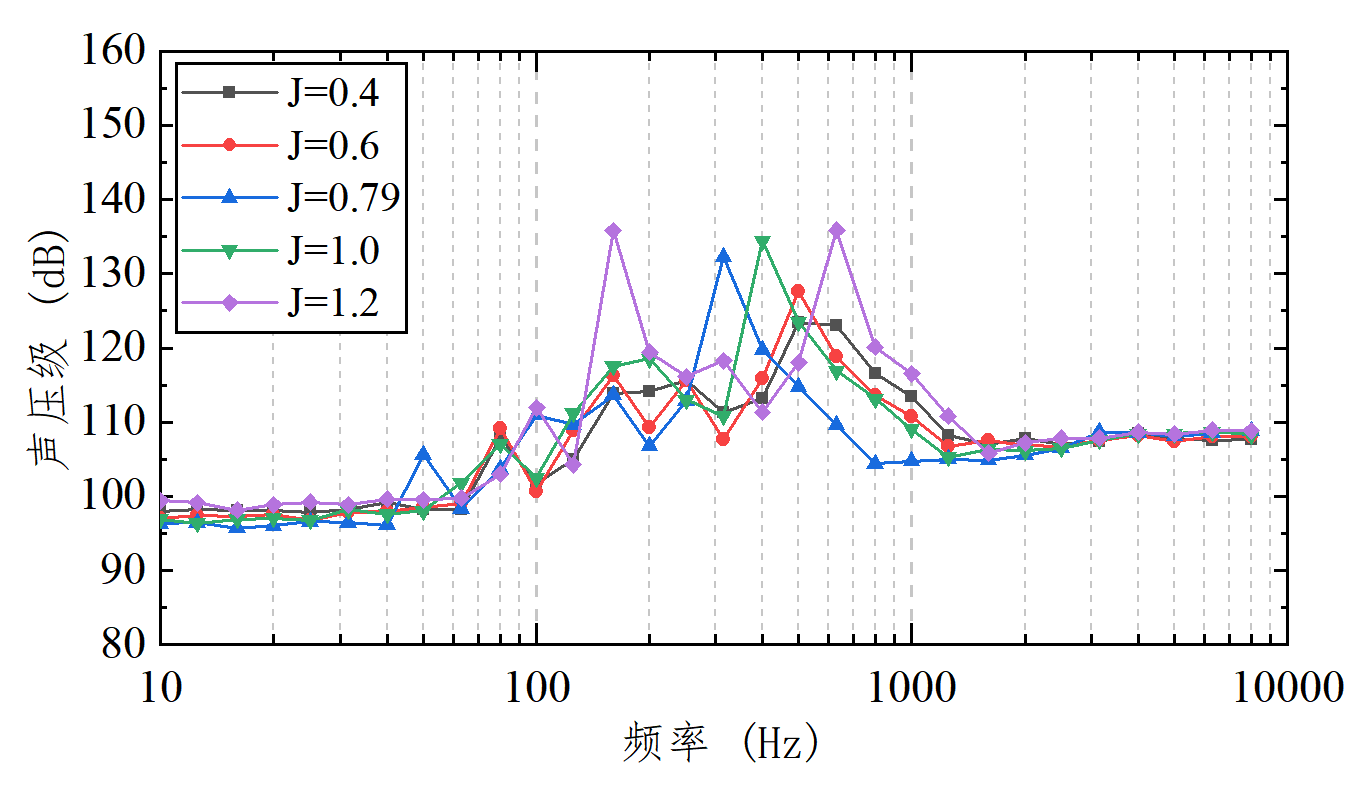
\includegraphics[scale=0.95]{3dj3_otc1.png}
    \caption{\label{fig:djotc2}单级推进泵噪声1/3倍频程分析(2号传感器)}
\end{figure}
\begin{figure}[htbp]
    \centering
    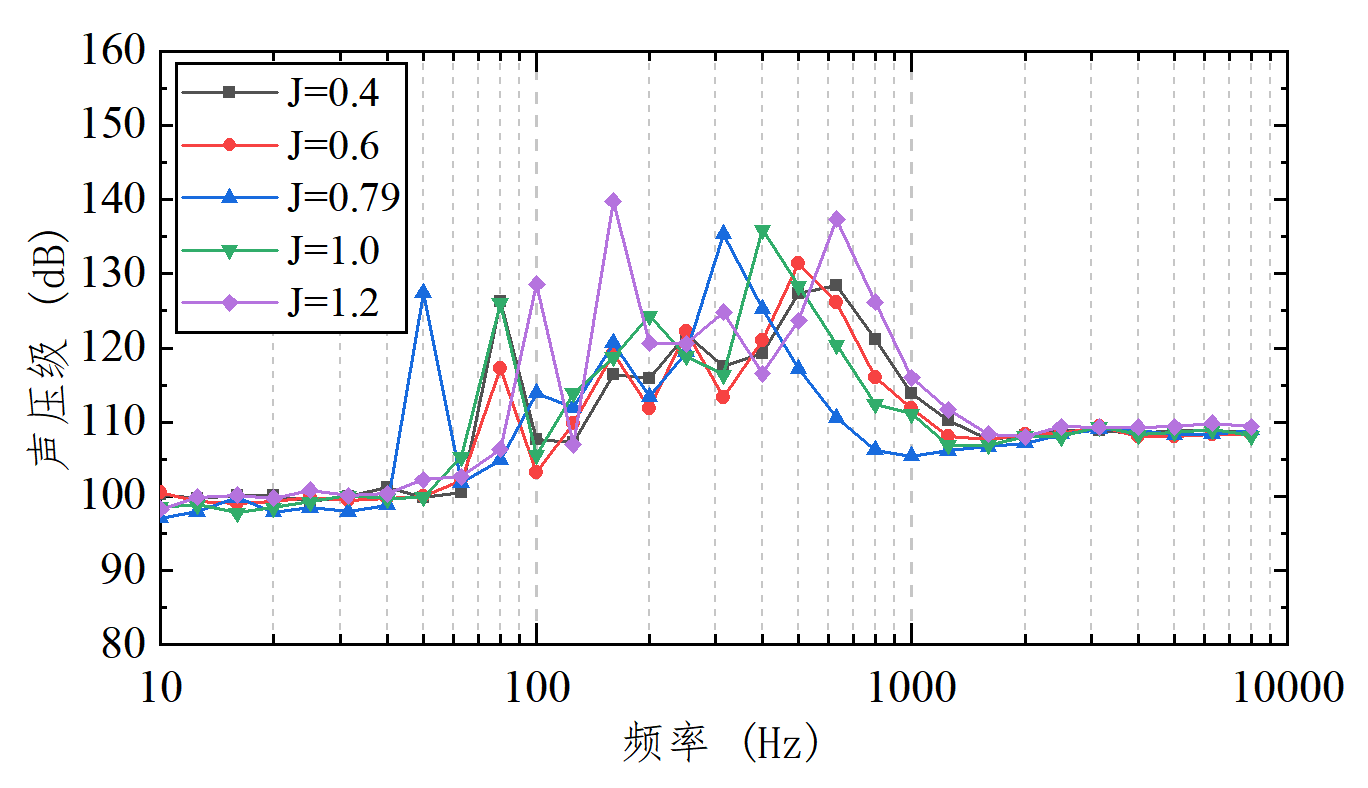
\includegraphics[scale=0.95]{3dj6_otc1.png}
    \caption{\label{fig:djotc3}单级推进泵噪声1/3倍频程分析(3号传感器)}
\end{figure}
\begin{figure}[htbp]
    \centering
    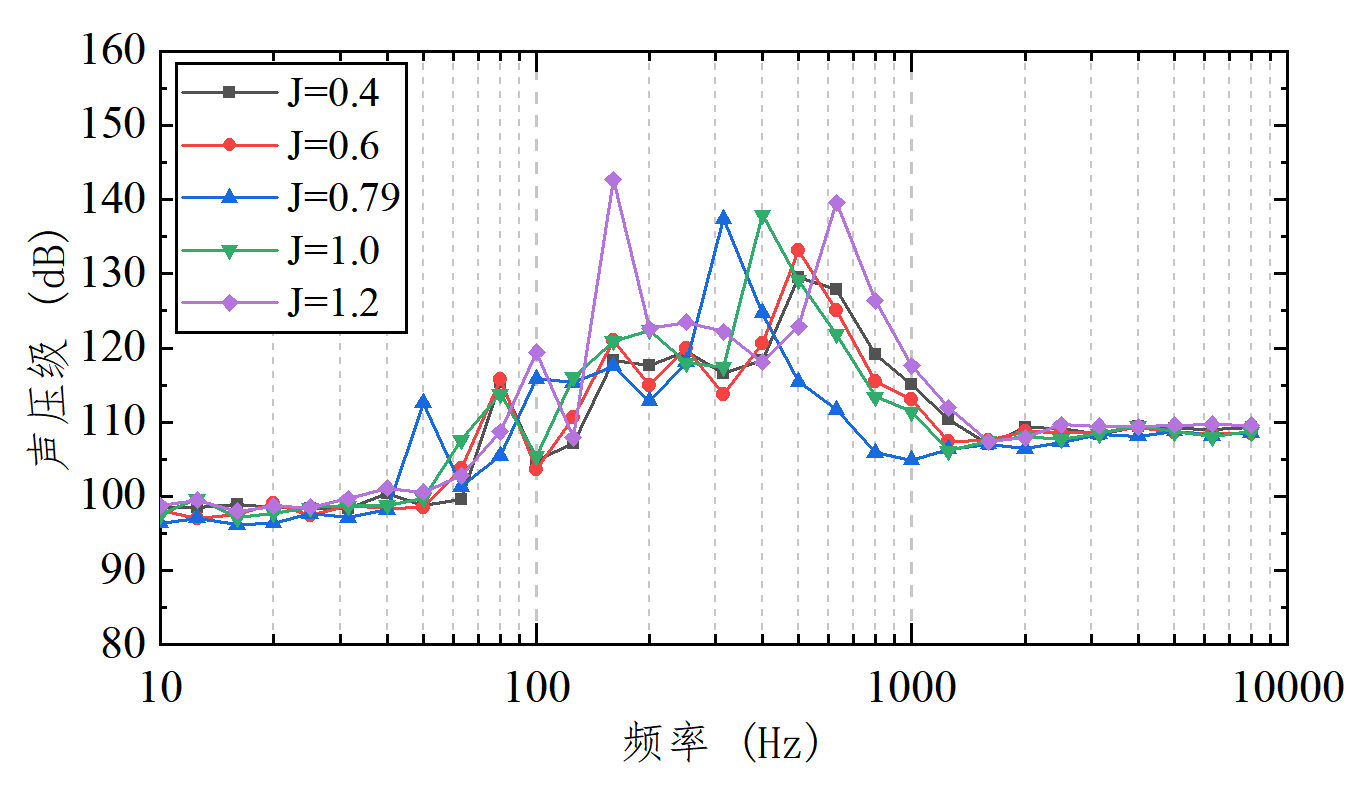
\includegraphics[scale=0.95]{3dj7_otc1.png}
    \caption{\label{fig:djotc4}单级推进泵噪声1/3倍频程分析(4号传感器)}
\end{figure}

如\autoref{fig:djotc1},\autoref{fig:djotc2},\autoref{fig:djotc3},\autoref{fig:djotc4}所示,
分别为单级推进泵在不同进速系数工况下,不同测点噪声信号的三分之一倍频程图。
与\autoref{fig:otcbeijing}背景噪声的三分之一倍频程图相比,
推进泵噪声的声压级幅值量级在中低频段有整体性的显著提升,其噪声能量在频域上的波动也更加剧烈。
如背景噪声能量波动的最大范围接近15dB,而推进泵噪声能量波动的最大范围已达到30dB。
在噪声能量分布方面,推进泵噪声能量波动主要发生在1 kHz以内的中低频段,高频段能量分布曲线平坦。
随着推进系数的增大,即流速的变大,声压级幅值最大的频段也在变化,
从而影响中低频段的能量分布。
随着流速的增大,高频段的曲线变化趋势不显著,说明流速变化对高频段的能量分布影响较小。
\begin{comment}
\begin{figure}[htbp]
        \centering
        \subfigure[pic1.]{
        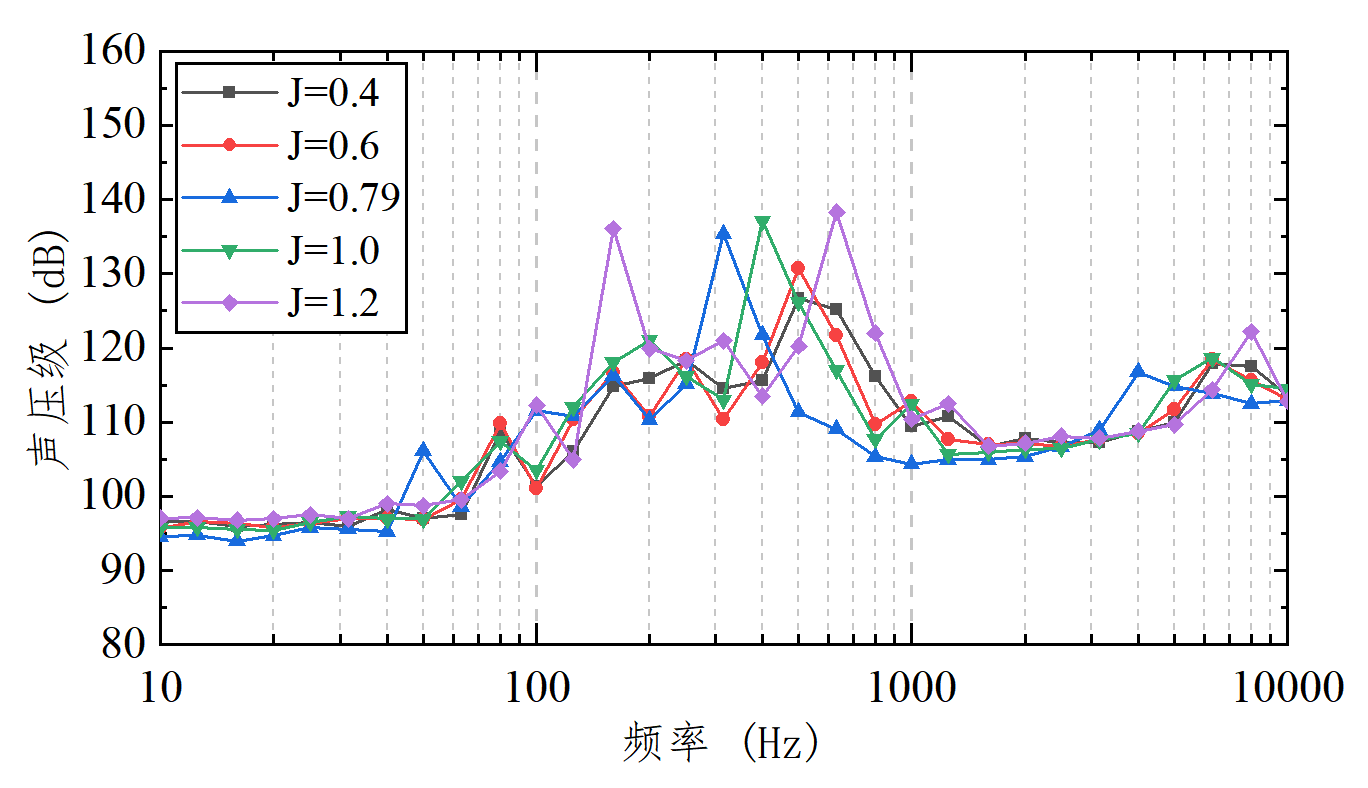
\includegraphics[scale=1.0]{3dj2_otc.png}
        }
\end{figure}
\addtocounter{figure}{-1}
\begin{figure}[htbp]
        \centering
        \addtocounter{figure}{1} 
        \subfigure[pic2.]{
        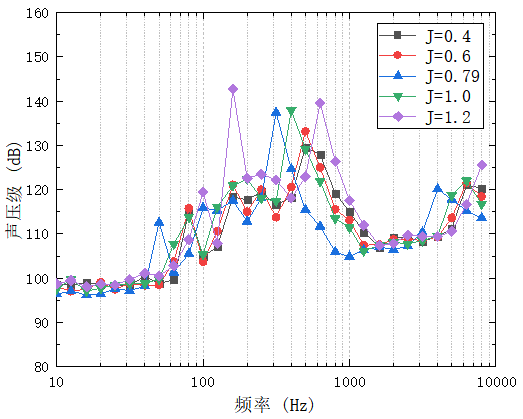
\includegraphics[scale=1.0]{3dj7_otc.png}
        }
        %\caption{\label{fig:dj_modle}不同工况下单级推进泵水下噪声三分之一倍频程图}
\end{figure}
\addtocounter{figure}{-1}
\begin{figure}[htbp]
        \centering
        \addtocounter{figure}{1} 
        \vspace{0.02cm}
        \subfigure[pic2.]{
        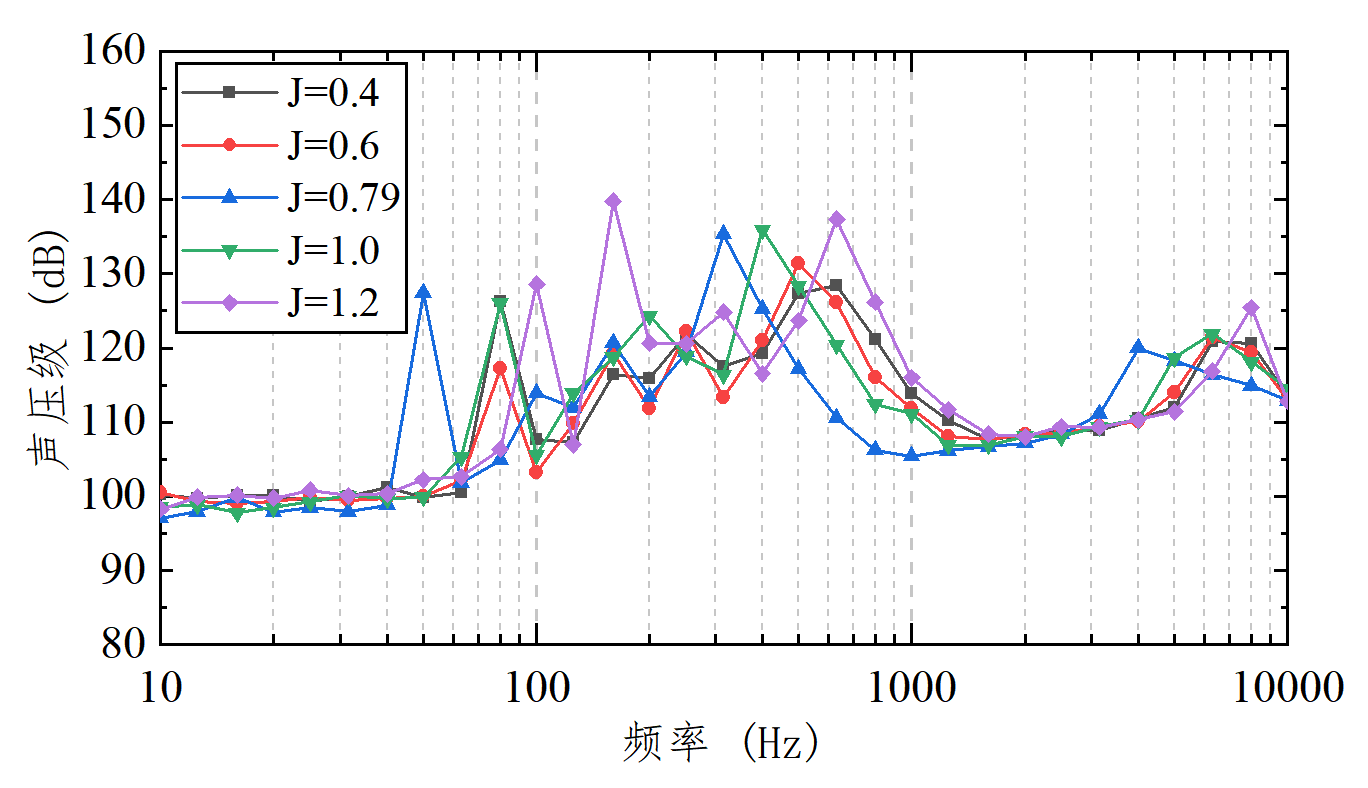
\includegraphics[scale=1.0]{3dj6_otc.png}
        }
        %\caption{\label{fig:dj_modle}不同工况下单级推进泵水下噪声三分之一倍频程图}
\end{figure}
\addtocounter{figure}{-1}
\begin{figure}[htbp]
        \centering
        \addtocounter{figure}{1} 
        \vspace{0.02cm}
        \subfigure[pic2.]{
        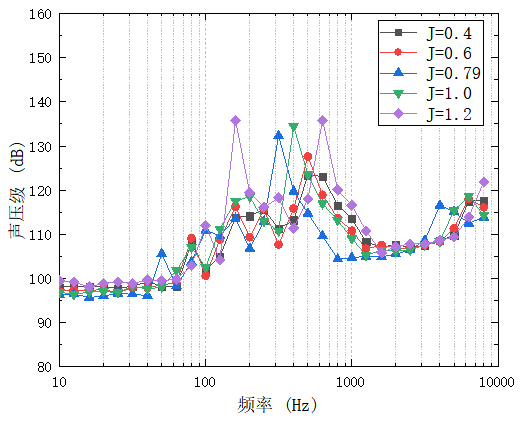
\includegraphics[scale=1.0]{3dj3_otc.png}
        }
        \caption{\label{fig:dj_modle}不同工况下单级推进泵水下噪声三分之一倍频程图}
\end{figure}
\end{comment}
\subsubsection{单级推进泵噪声特征频段分析}
为了进一步评估流速对推进泵特征频段的影响,以及各个特征频段对噪声总级的贡献度。
基于噪声测试系统中的数据分析模块,可获得各测点不同频段的声压级平均值,平均方法如\autoref{equ:Lave}所示。
\begin{equation}
    \label{equ:Lave}
    L_{ave}=10\log_{10}\left ( {10^{0.1L_{p1}}}+{10^{0.1L_{p2}}}+{10^{0.1L_{p3}}}+{10^{0.1L_{p4}}}  \right ) 
\end{equation}

如\autoref{fig:djtotal}所示为推进泵噪声在不同工况下噪声总声压级。
从图中可以看出,随着进速系数的变大,各个频段的声压级单调递增。
对比水洞背景噪声的特征频段总声压级变化,可以发现在低流速工况时,推进泵的噪声总声压级和背景噪声相近,
说明此时推进泵噪声信号信噪比低。
当流速从1.26m/s增大到5.05m/s时,背景噪声的声压总级增幅为7.2dB,推进泵声压总级的增幅为12.2dB。

在考虑背景噪声影响的基础上,推进泵噪声的总声压量级仍然会随流速的增大而增大。
此外,流速的增大不仅对全频段的声压级有增强作用,
还会提升推进泵噪声低中高三个频段的能量。
其中,流速的变化对低频段(10Hz-100Hz)和高频段(1kHz-10kHz)的总声压级影响较小,当水速从1.26m/s增大到
5.05m/s时,低频段和高频段的总声压级的增幅分别为3.1dB和2.0dB。
考虑背景噪声的影响,水速对中频段(100Hz-1kHz)的总声压级影响更为显著,当水速从1.26m/s增大到5.05m/s时,
中频段的总声压级增幅达到5.0dB。
不同工况下中频段(100Hz-1kHz)、中低频段(10Hz-1kHz)和全频段(10Hz-10kHz)的变化曲线几乎重合,
这说明中低频段噪声是推进泵噪声最主要的贡献量。
\begin{figure}[htbp]
    \centering
    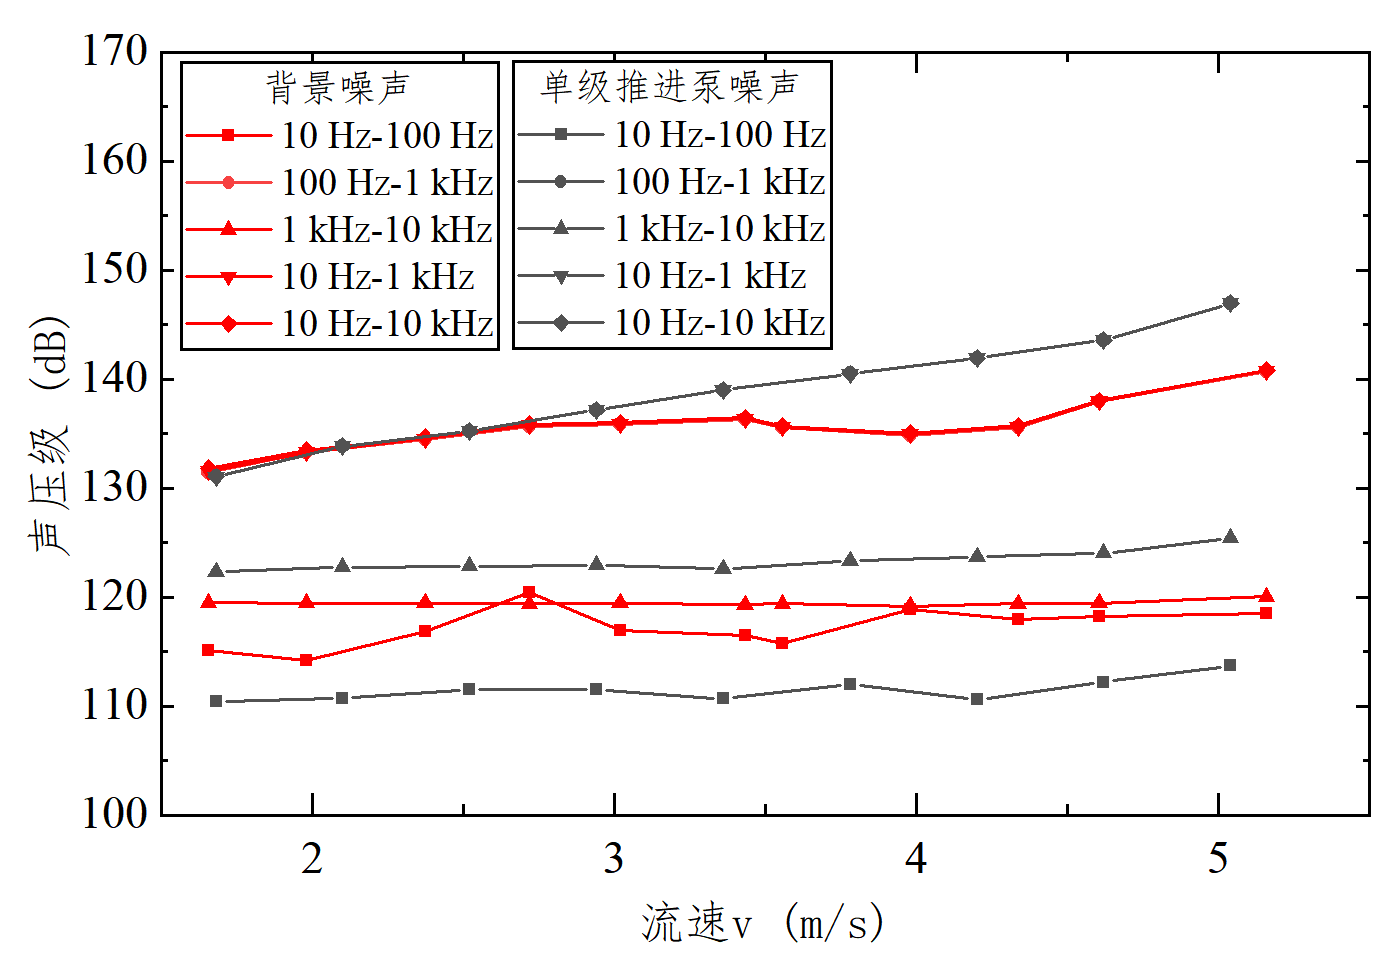
\includegraphics[scale=1]{3单级总声压2.png}
    \caption{\label{fig:djtotal}单级推进泵噪声在不同工况下各个频段的噪声总声压级}
\end{figure}
\subsubsection{单级推进泵噪声频谱分析}
随机选取了2号测点各工况下的噪声信号进行频谱分析,由上小节分析可知噪声频谱能量波动主要集中在中低频段,
因此本文重点讨论2000Hz以内的频谱特征。
分析结果中对频率作了无量纲化处理,即采用轴系转速进行无量纲化($f/f_n$)。
为了更好的表述频谱中的特征频率,
将单级推进泵的轴频定义为APF(对应$f_n$),叶轮叶频定义为BPF(对应7$f_n$),导叶叶频表示为SBPF(对应11$f_n$)。
\begin{figure}[htbp]
    \centering
    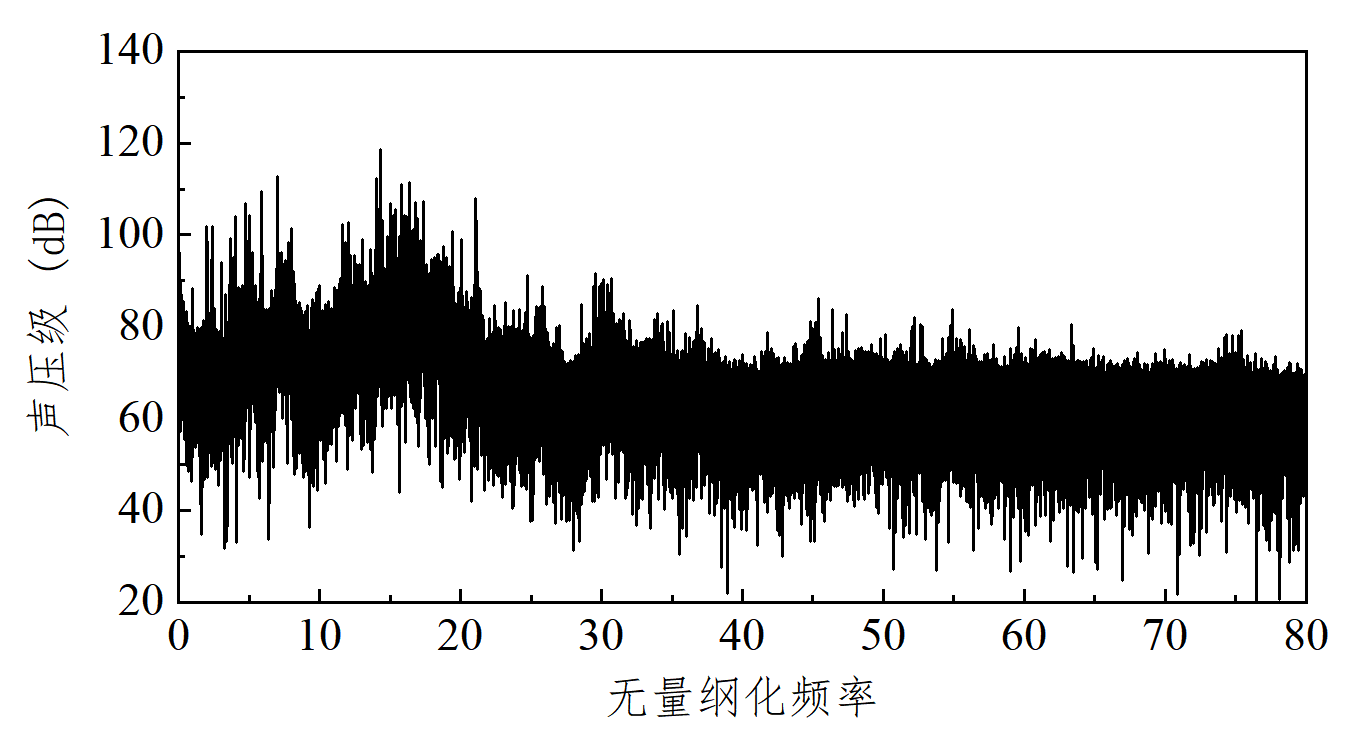
\includegraphics[scale=1]{3dj0.4频谱1.png}
    \caption{\label{fig:dj0.4}J=0.4工况下单级推进泵噪声频谱}
\end{figure}
\begin{figure}[htbp]
    \centering
    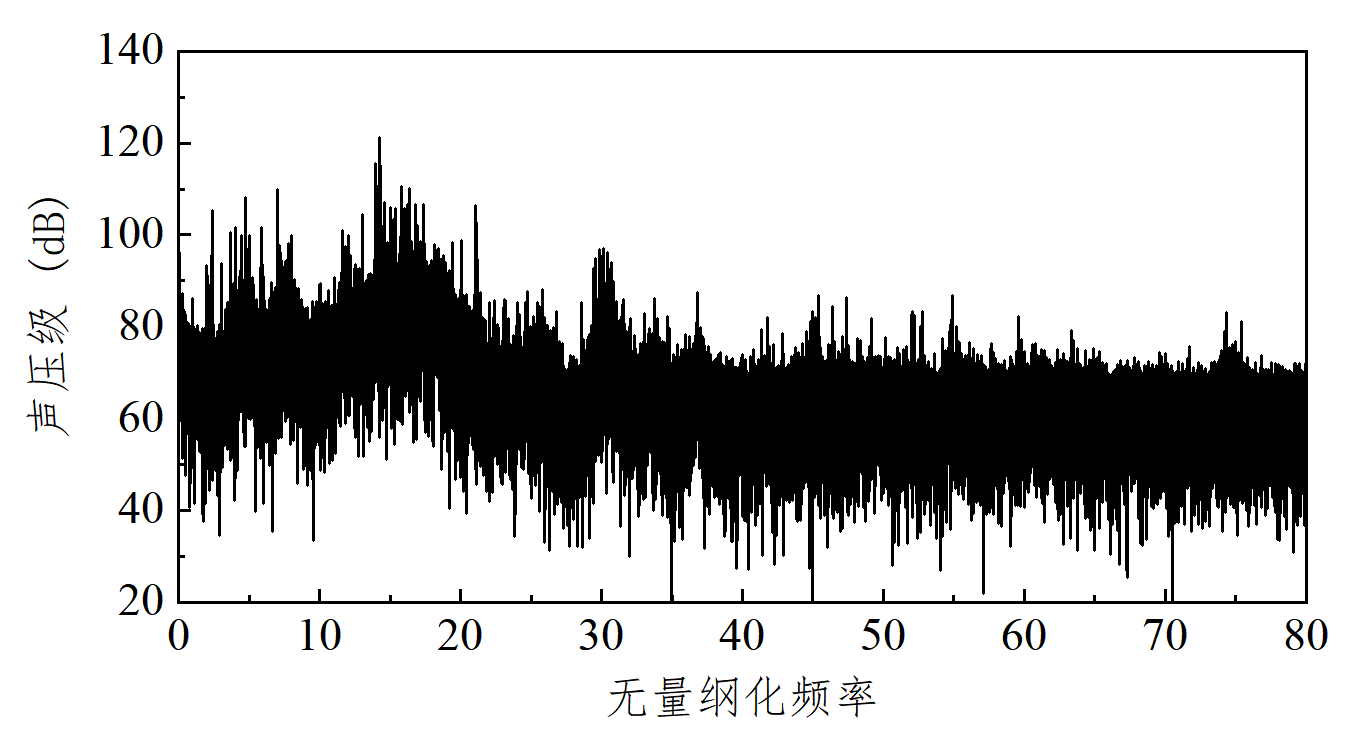
\includegraphics[scale=1]{3dj0.6频谱1.png}
    \caption{\label{fig:dj0.6}J=0.6工况下单级推进泵噪声频谱}
\end{figure}
\begin{figure}[htbp]
    \centering
    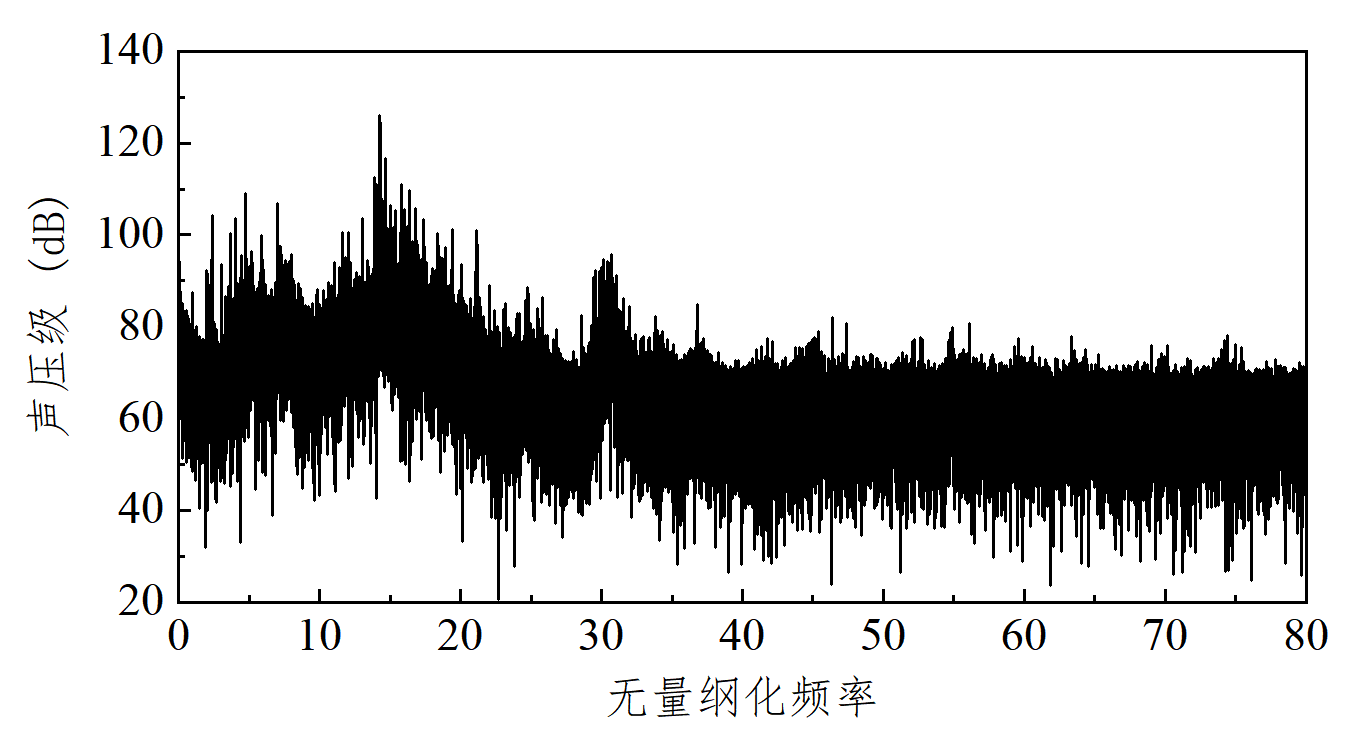
\includegraphics[scale=1]{3dj0.79频谱1.png}
    \caption{\label{fig:dj0.79}J=0.79工况下单级推进泵噪声频谱}
\end{figure}

如\autoref{fig:dj0.4},\autoref{fig:dj0.6},
\autoref{fig:dj0.79},\autoref{fig:dj1},\autoref{fig:dj1.2}所示,
分别在不同进速系数工况下的单级推进泵噪声的频谱图。
可以看出监测到的推进泵噪声频谱特性表现为中低频线谱噪声、中低频宽带噪声和高频宽带噪声。
由于单级推进泵噪声的能量主要集中在中低频段,频谱中的中低频线谱幅值显著高于宽带噪声,这说明中低频线谱对推进泵噪声有显著贡献。
\begin{figure}[htbp]
    \centering
    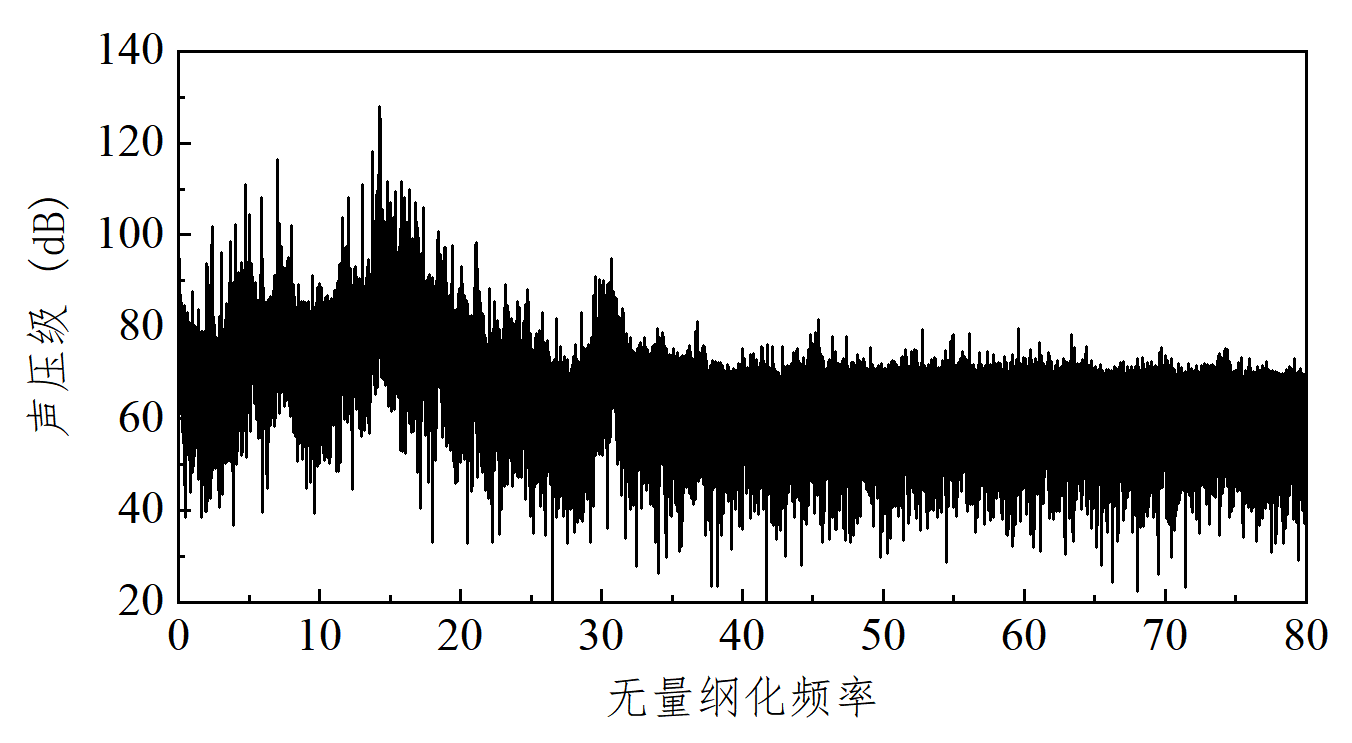
\includegraphics[scale=1]{3dj1.0频谱1.png}
    \caption{\label{fig:dj1}J=1.0工况下单级推进泵噪声频谱}
\end{figure}
\begin{figure}[htbp]
    \centering
    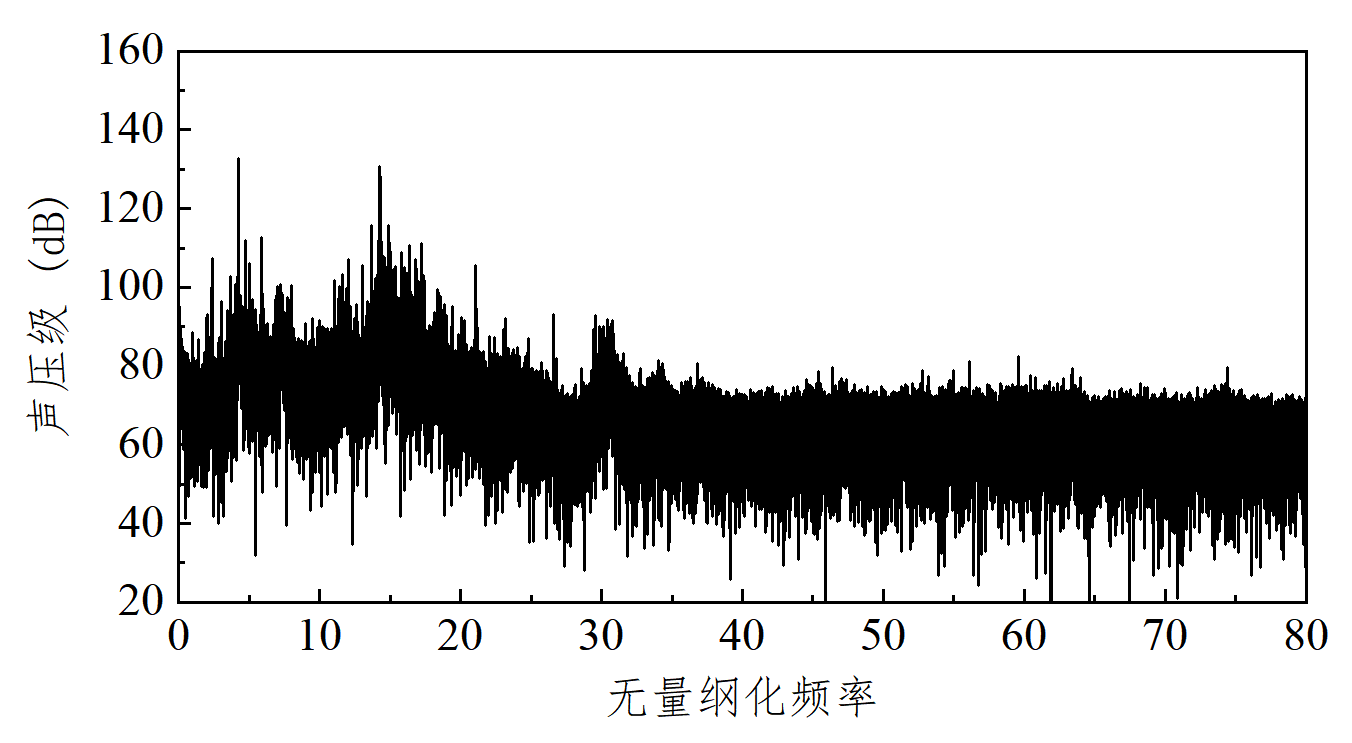
\includegraphics[scale=1]{3dj1.2频谱1.png}
    \caption{\label{fig:dj1.2}J=1.2工况下单级推进泵噪声频谱}
\end{figure}

结合\autoref{fig:djotc1}至\autoref{fig:djotc4}推进泵噪声三分之一倍频程可以看出,频段能量分布的波动与线谱成分有较大关联。
中低频段线谱成分丰富,中低频段比较明显的线谱有BPF,2BPF,3BPF,其中2BPF线谱的幅值要高于BPF和3BPF。
在APF-30APF之间还存在以APF为间隔的连续线谱成分,如4APF,5APF,6APF等较为突出的线谱。
除了这些特征线谱外,中低频段还有很多幅值不显著的复杂线谱成分,
其中也包括背景噪声带来的干扰频率成分。

此外,中低频段频谱中也能观察到微弱的轴频APF成分,该线谱成分几乎淹没在频谱中。
在流速较小的工况下,噪声信噪比较低,BPF、2BPF等特征频率与其周围线谱幅值相差不大,不能准确且快速的识别出来。
2BPF,3BPF等特征线谱随着流速的增大,在频谱中越容易被识别出来。
随着流速的增大,APF-10APF之间的轴频谐波成分和2BPF,3BPF等特征线谱处的幅值变化无明显规律。

综上,单级推进泵噪声频谱特性表现为中低频线谱噪声、中低频宽带噪声和高频宽带噪声。
噪声能量主要集中在中低频段,中低频线谱影响着噪声能量的分布,对推进泵噪声总声压级有显著贡献。
频谱中线谱成分丰富,以轴频和叶频的谐波成分为主,其中2BPF线谱的幅值要高于BPF和3BPF。
在噪声信噪比较低的工况下,APF、BPF和2BPF等低频线谱特征在频谱中不能准确且快速的被识别。
噪声中低频段、高频段和全频段的总声压级随着流速的增大而增大,流速变化对推进泵噪声高频段的能量分布和总声压级影响较小,
对中低频段的能量分布和总声压级影响更加明显。

\section{双级推进泵噪声特性的试验研究}
\subsection{推进泵试验模型}
本小节的研究对象是一种新型结构推进泵。其设计引入多级泵的设计思路,采用一根轴驱动两个叶轮,
再通过中间的导叶来回收环量。该双级推进泵通过采用特殊的两级叶轮形式降低推进器转速,提高能量密度。
与上小节的单级推进泵一样,其设计参数也是根据某航行体的推进需求计算,并进行缩尺得到。
在单级推进泵的设计基础上,最终确定双级推进泵的轮缘直径为200mm,其直径空间与单级推进泵一致。
\begin{figure}[htbp]
    \centering
    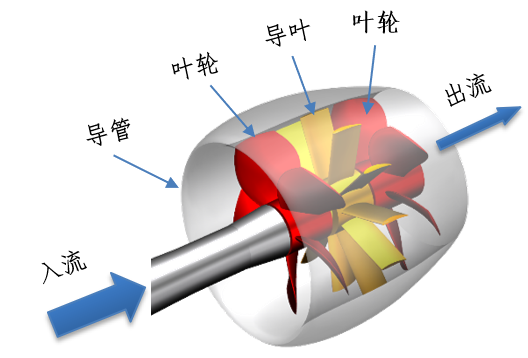
\includegraphics[scale=1.0]{5双级整体结构.png}
    \caption{\label{fig:sj_modle}双级推进泵设计模型}
\end{figure}

导管的设计选用 33 号减速喷管,可在一定程度上降低入流速度充分提升叶轮
的抗空化性能,并根据动量定理确定导管得出口直径,保证推进器能产生足够的推力。
叶轮的设计主要考虑了以下几个方面:
(1)在叶型剖面角度设计中,选用了较小的冲角,目的是在保证推进效率的前提下,更大程度地提高推进器的抗空化与声学性能;
(2)采用了较大的叶片落后角,可以使叶片在有限的轴向长度内具有更大的做功能力,以充分提升双级推进泵的能量密度;
(3)中间导叶采用C型设计,可以有效地回收利用前叶轮出口的切向速度,并为后转子提供预旋,减小甚至消除推进系统出口的环量,以提高推进器的效率。
双级推进泵设计模型如\autoref{fig:sj_modle}所示,双级推进泵的设计参数如\autoref{tab:sj}所示。
\begin{figure}[htbp]
    \centering
    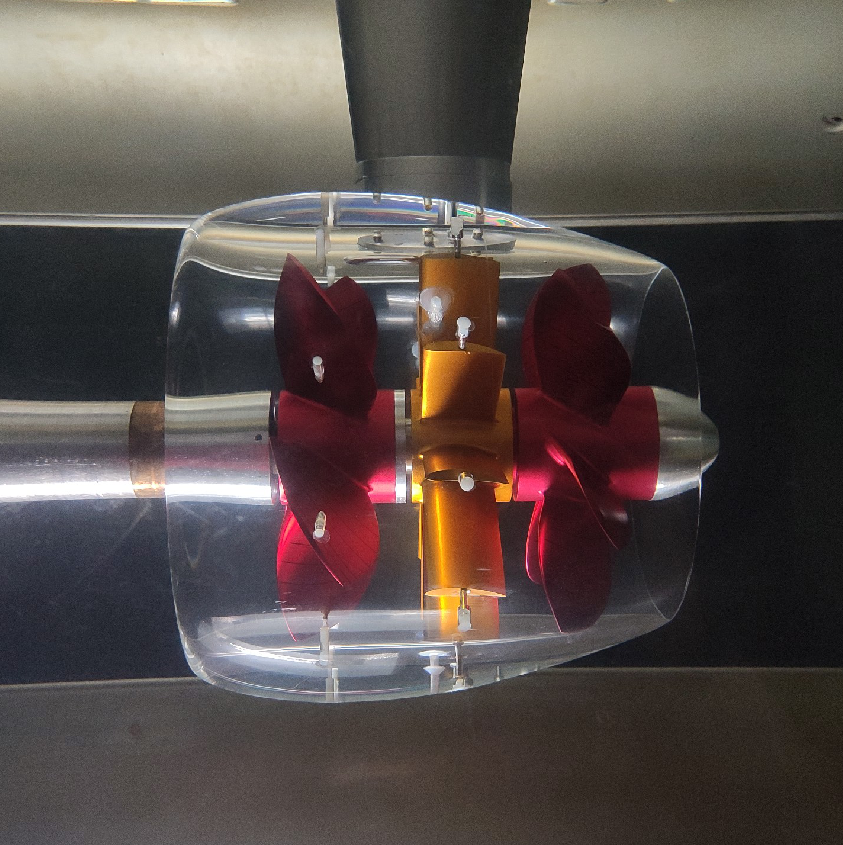
\includegraphics[scale=0.25]{3双级试验模型.png}
    \caption{\label{fig:sj_test}双级推进泵试验模型}
\end{figure}

\begin{table}[htbp]
    \centering
    \caption{\label{tab:sj}双级推进泵设计参数}
    \begin{tabular}{ccc}
     \toprule
     参数&值\\
     \midrule
     D(叶轮直径,mm)&200\\
     N(设计转速,rpm)&970\\
     L(导管长度,mm)&240\\
     $D_1$(入口直径,mm)&228\\
     $D_2$(出口直径,mm)&182\\
     $Z_1$(首级叶轮叶片数)&5\\
     $Z_s$(导叶叶片数)&11\\
     $Z_2$(次级叶轮叶片数)&6\\
     轮毂比&0.3\\
     旋向&右旋\\
     %APF(轴频,Hz)&16.17\\
     %BPF$_1$(首级叶轮叶频,Hz)&80.85\\
     %BPF$_2$(次级叶轮叶频,Hz)&97.02\\
     %SBPF(导叶叶频,Hz)&177.87\\
     \bottomrule
    \end{tabular}
\end{table}

推进器整体外形为流线型筒体,两级叶轮和导叶均装于筒体内。推进器前后两级叶轮位于导叶两侧,导叶体起到导流与支撑作用。
推进器叶轮采用铝合金加工制造,表面做阳极化处理。导管选用有机玻璃材质,表面做抛光处理,导管内壁与转叶叶梢间隙约1mm。
双级推进泵试验模型如\autoref{fig:sj_test}所示。
\begin{figure}[htbp]
    \centering
    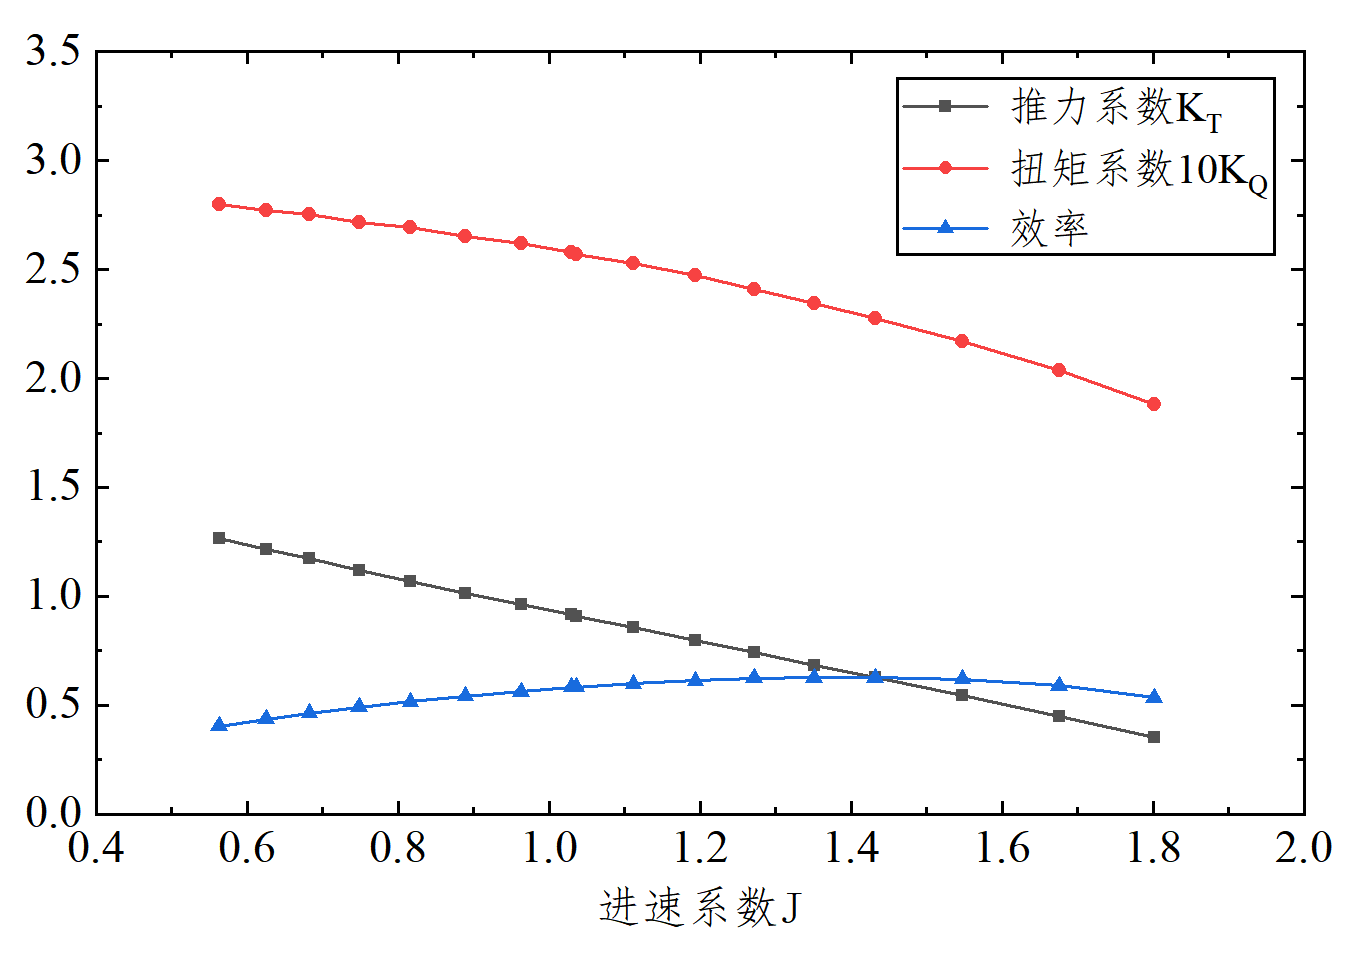
\includegraphics[scale=1]{3双级敞水性能.png}
    \caption{\label{fig:sj_changshui}双级推进泵敞水性能曲线}
\end{figure}

将水洞试验测得的双级推进泵推力、转矩和效率等数据无量纲化后,得到如\autoref{fig:sj_changshui}所
示的敞水性能曲线。从图中可以看出:随着进速系数J的增大,
推力系数$K_T$和转矩系数$K_Q$逐渐减小,而推进效率$\eta_0$先增大后减小,
并在 J=1.35 处有最大值 62.7\%。与常见的螺旋桨敞水性能
曲线相比,双级推进泵的敞水性能曲线随进速系数增加时变化趋势平缓,具有较高推进
效率的同时也有较宽的高效工作区。
\begin{figure}[htbp]
    \centering
    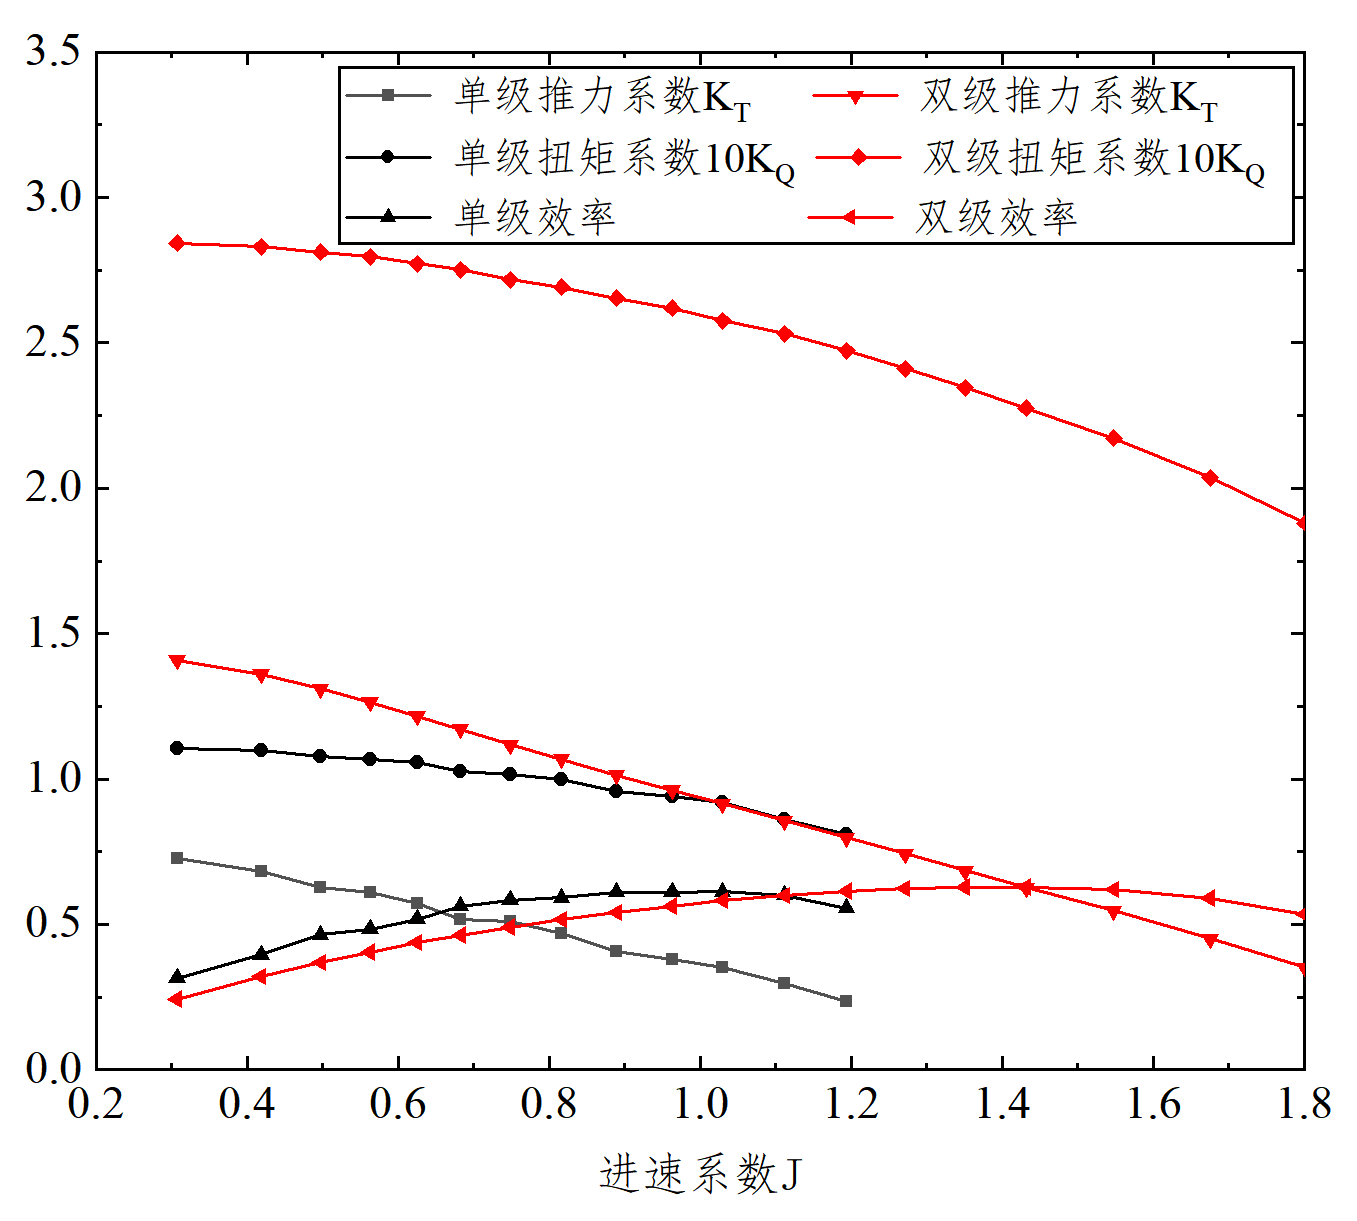
\includegraphics[scale=1]{3单双级敞水性能对比.png}
    \caption{\label{fig:sj_dj}双级推进泵与单级推进泵敞水性能曲线对比}
\end{figure}

与上小节研究的单级推进泵相比,两种推进泵的敞水性能曲线对比如\autoref{fig:sj_dj}所示。
在相同的直径空间下,双级推进泵的推力和转矩基本上相当于两台普通单级推进器。
此外,可以看到,单级推进泵的效率性能曲线在J=1.2的时候效率就开始下降了,而双级推进泵的效率性能曲线到1.8才开始下降。
双级推进泵的特性曲线变化更加平缓,这就使其高效区域更宽,
并且在高进速系数时仍可以保持较高效率,
说明双级推进器在高进速系数时仍可以保持较高效率。
有限的直径空间内,双级推进泵在降低转速的同时也有效提高了能量密度,适用于负荷较重的水面、水下航行器。

在噪声试验方面,采用水听器型号依旧为丹麦 Reson TC4013,采集装置和单级推进泵一致,
利用水听器阵列进行推进泵辐射噪声的采集,其固定实验装置如\autoref{fig:sjstq}所示,
加工好的木板在水舱中与水洞侧壁面平行放置,水听器垂直置于木板孔中,
图上标号表示水听器的安放位置。基于噪声测试系统对上述位置的噪声信号进行同步采集,
采样频率为40960Hz,每次测试采样时间为10s。
\begin{figure}[htbp]
    \centering
    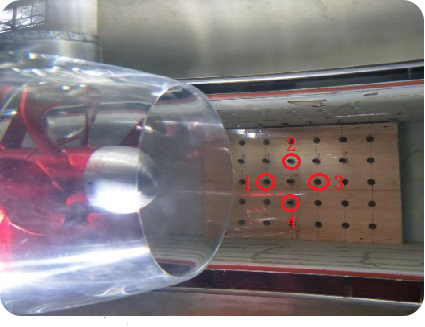
\includegraphics[scale=1.0]{3单级水听器布置.png}
    \caption{\label{fig:sjstq}双级推进泵噪声试验中水听器布置}
\end{figure}
\subsection{推进泵噪声特性分析}
试验中通过固定叶轮转速16.67rps、改变水洞流速的方法测量了进速系数0.3至1.8范围内20个工况点下的
水动力性能和噪声数据,对应流速从1.02m/s增加至6.01m/s范围内的工况点。
本文选取进速系数分别为0.5,0.8,1.0,1.3和1.5,
对应水速分别为1.68m/s,2.52m/s,3.32m/s,4.2m/s和5.05m/s工况下的噪声数据进行分析。
基于噪声测试系统中的数据分析模块,获得了推进泵噪声的三分之一倍频程和频谱分析结果。
本小节噪声范围的划分与单级推进泵保持一致,低频噪声的频率范围划分为100Hz以下,高频噪声在1000Hz以上,而低频与高频之间过渡频
段的噪声划分为中频噪声。
\subsubsection{双级推进泵噪声三分之一倍频程分析}

\begin{figure}[htbp]
    \centering
    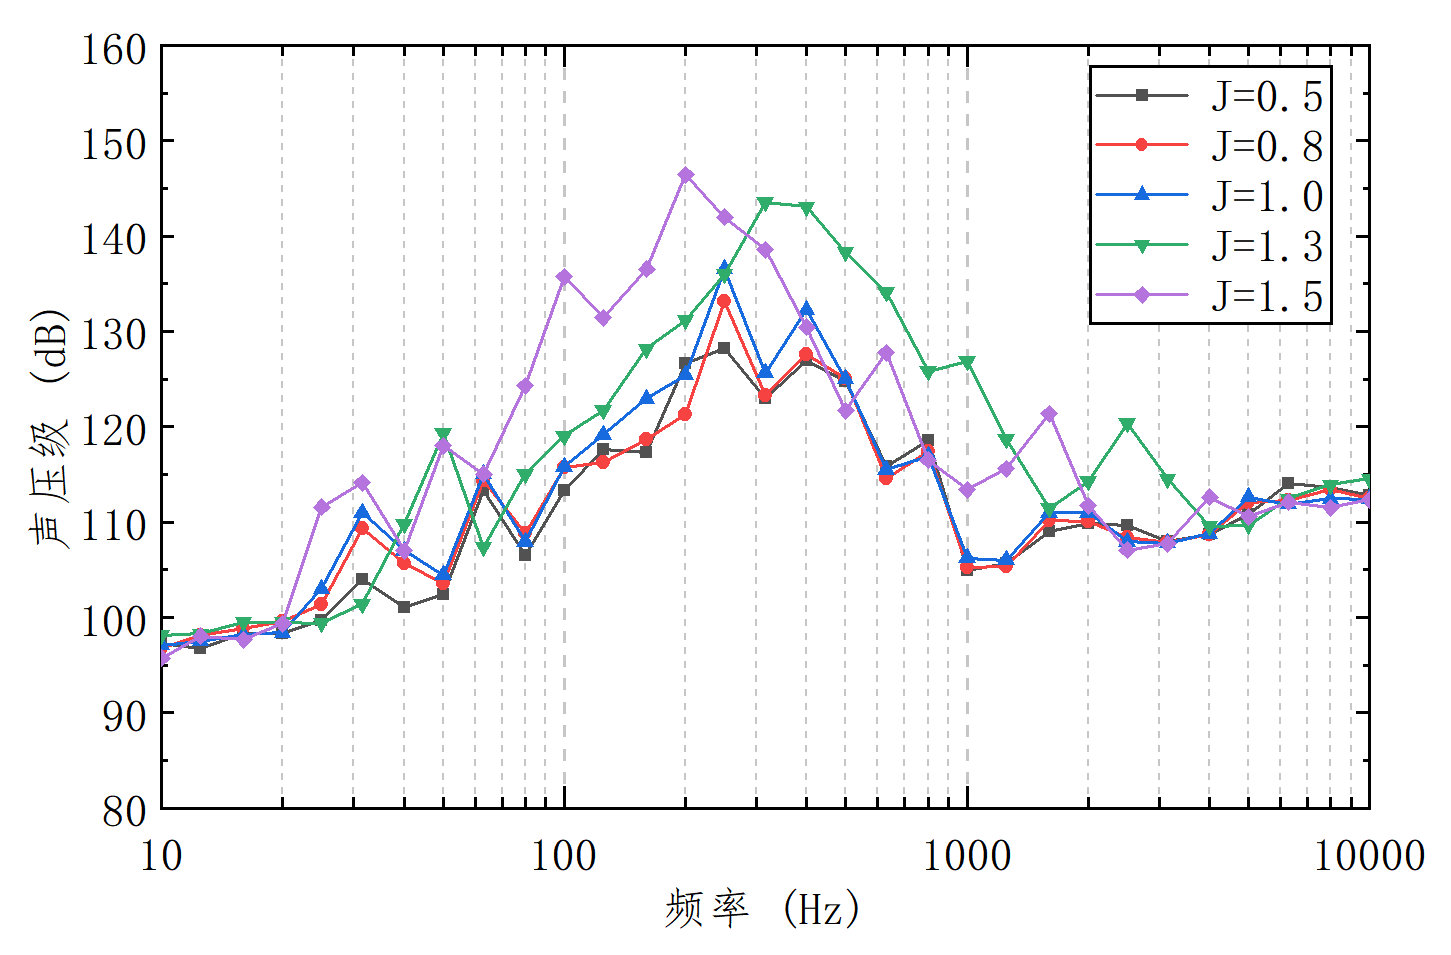
\includegraphics[scale=0.95]{3sj倍频程3.png}
    \caption{\label{fig:sjotc1}双级推进泵噪声1/3倍频程分析(1号传感器)}
\end{figure}
\begin{figure}[htbp]
    \centering
    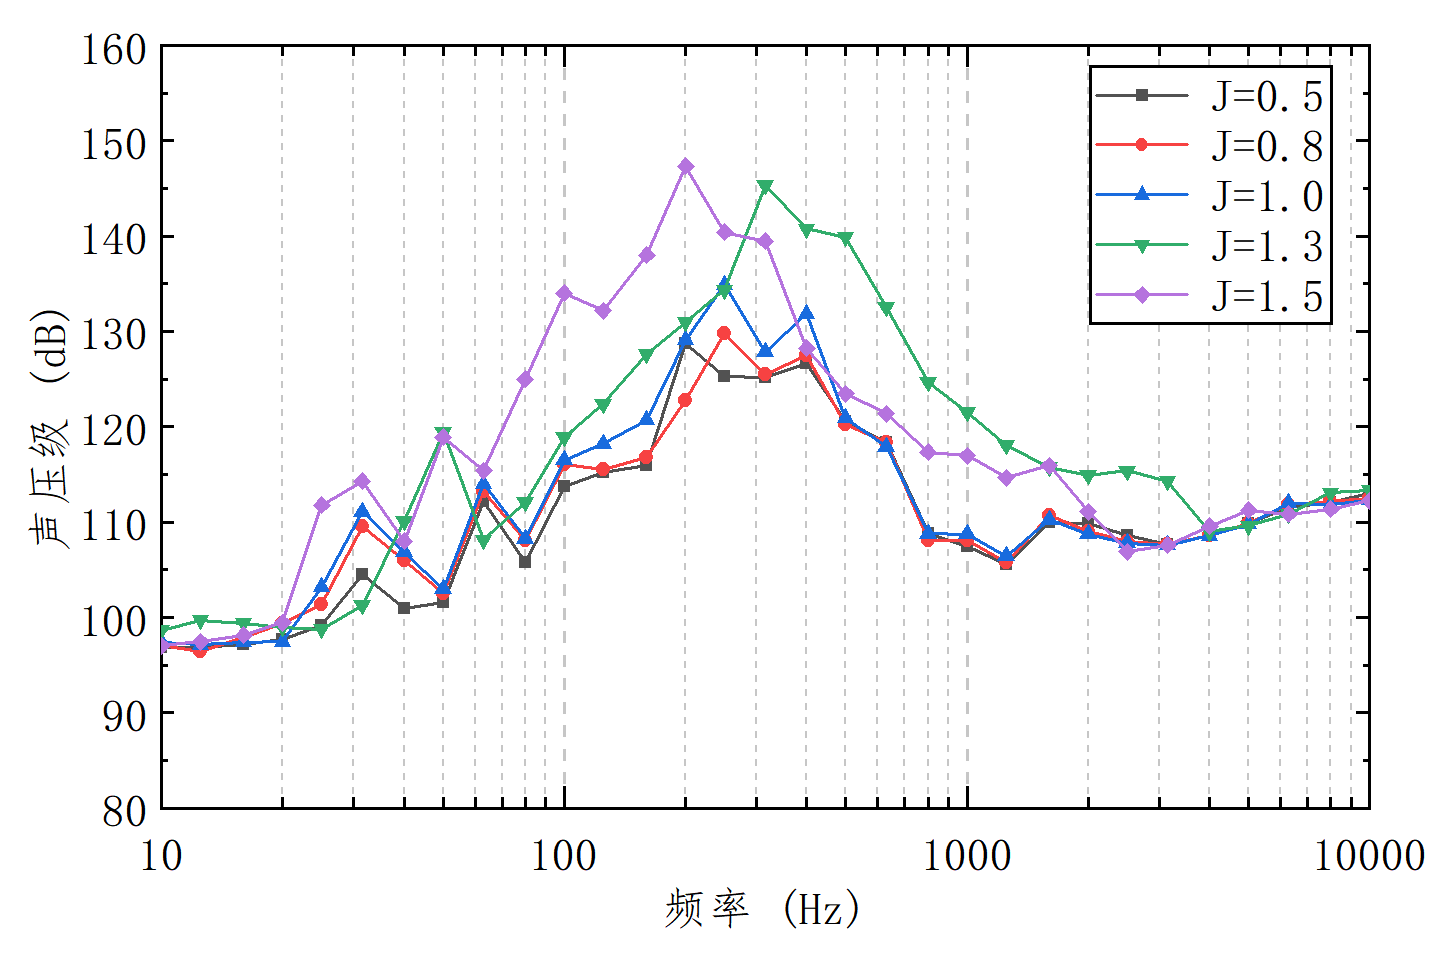
\includegraphics[scale=0.95]{3sj倍频程4.png}
    \caption{\label{fig:sjotc2}双级推进泵噪声1/3倍频程分析(2号传感器)}
\end{figure}
\begin{figure}[htbp]
    \centering
    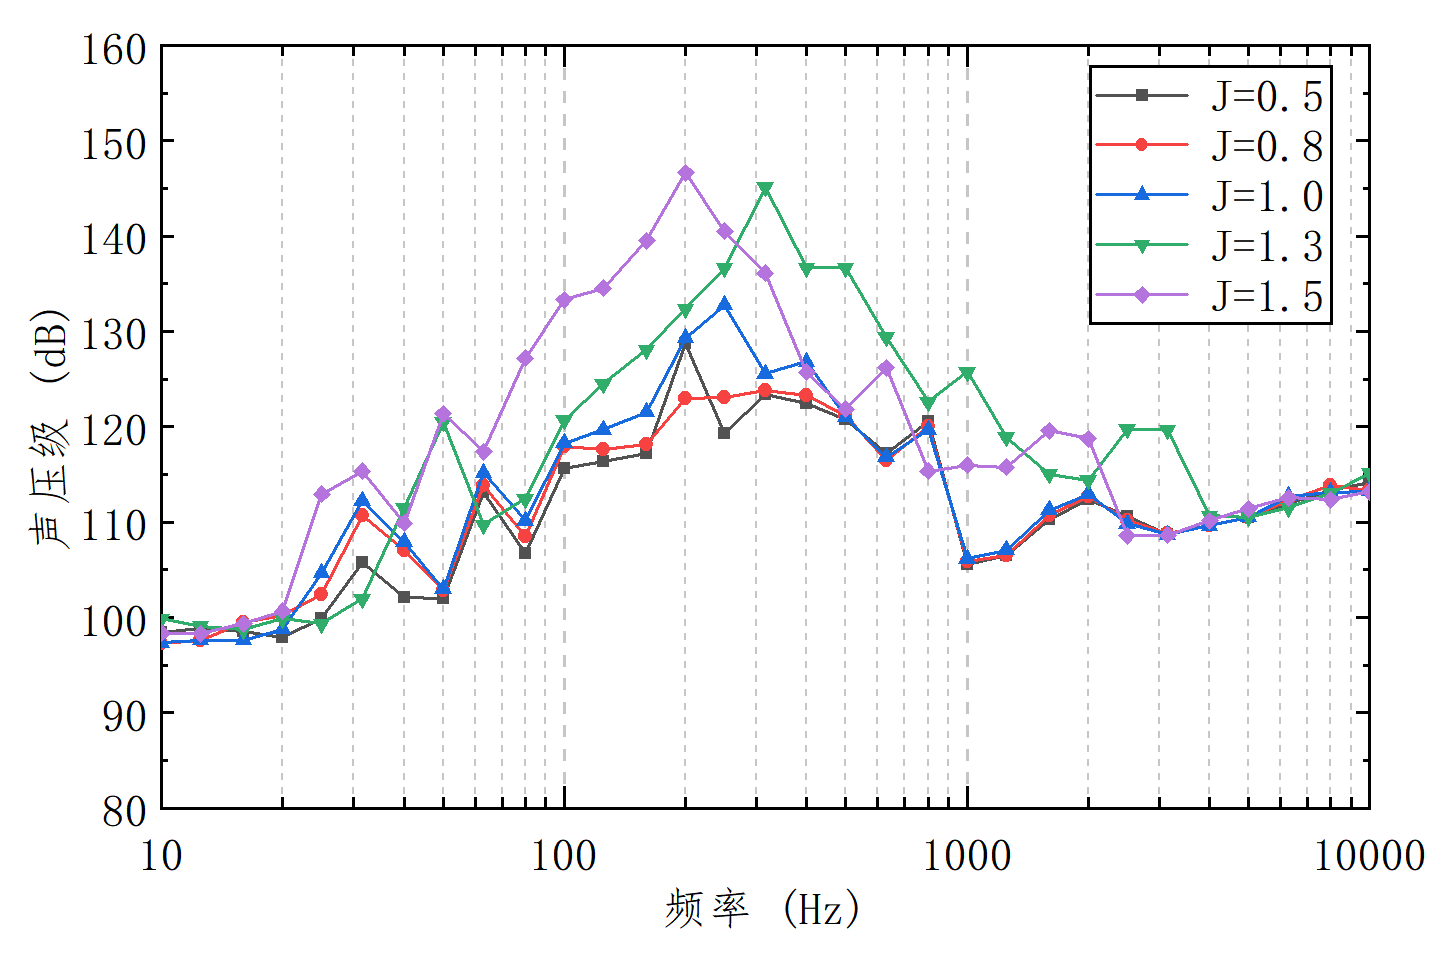
\includegraphics[scale=0.95]{3sj倍频程5.png}
    \caption{\label{fig:sjotc3}双级推进泵噪声1/3倍频程分析(3号传感器)}
\end{figure}
\begin{figure}[htbp]
    \centering
    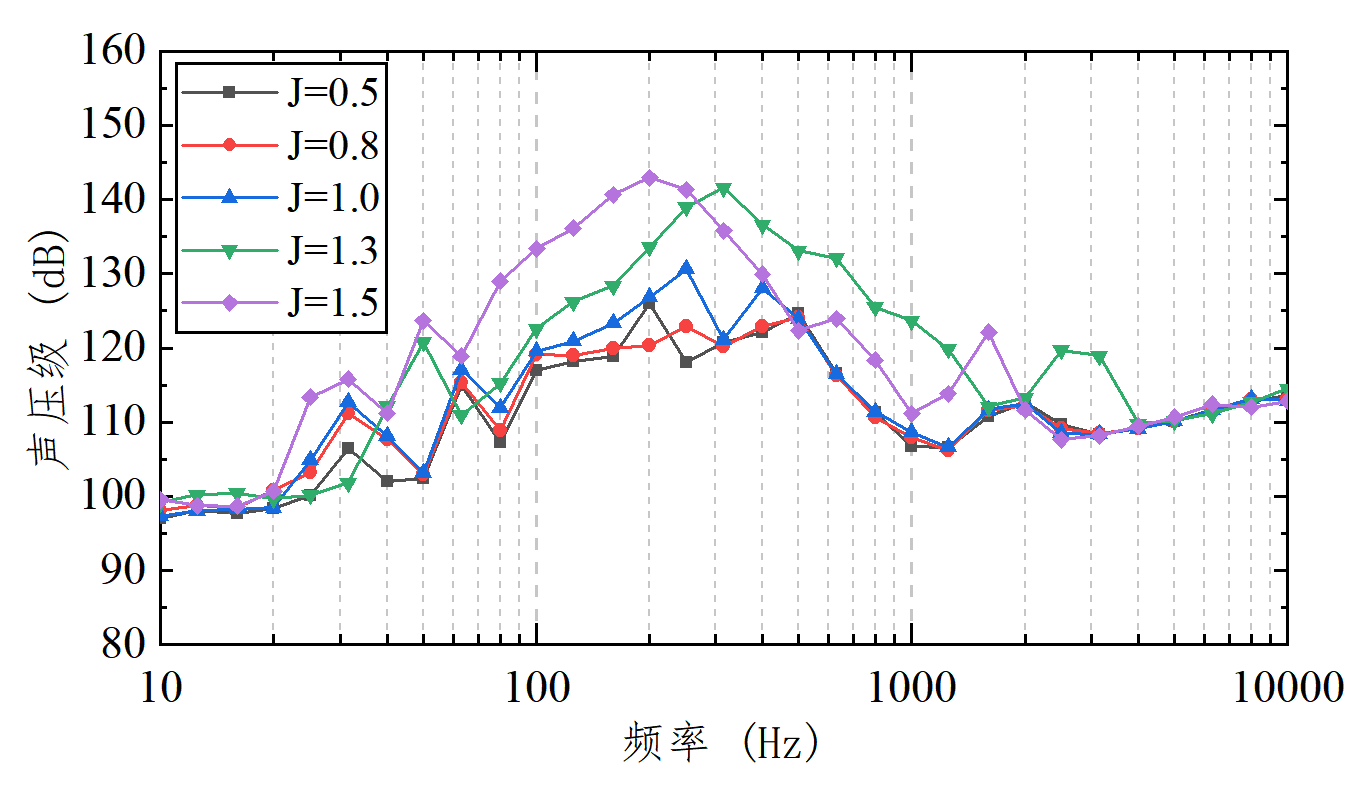
\includegraphics[scale=0.95]{3sj倍频程6.png}
    \caption{\label{fig:sjotc4}双级推进泵噪声1/3倍频程分析(4号传感器)}
\end{figure}

如\autoref{fig:sjotc1},\autoref{fig:sjotc2},\autoref{fig:sjotc3},\autoref{fig:sjotc4}所示,
分别为双级推进泵在不同进速系数工况下,不同测点噪声信号的三分之一倍频程图。
与\autoref{fig:otcbeijing}背景噪声的三分之一倍频程图相比,
双级推进泵噪声的声压级幅值量级在中低频段有整体性的显著提升,其噪声能量在频域上没有突出的上下波动,
噪声能量分散到更宽的频带上。

在噪声能量分布方面,推进泵噪声能量波动主要发生在1 kHz以内的中低频段,高频段能量分布曲线平坦。
可以看出噪声能量主要集中在中低频段。
在中低频段,推进泵噪声能量分布表现出先稳步增长,后逐步下降的趋势,其噪声频谱具有更好的平稳性。
随着推进系数的增大,即流速的变大,几乎中低频段的各个频段声压级幅值也在提升。
这说明流速对中低频段能量的影响体现在中低频整个频段上。
随着流速的增大,高频段的曲线变化趋势不显著,说明流速变化对高频段的能量分布影响较小。

\subsubsection{双级推进泵噪声特征频段分析}
\begin{figure}[htbp]
    \centering
    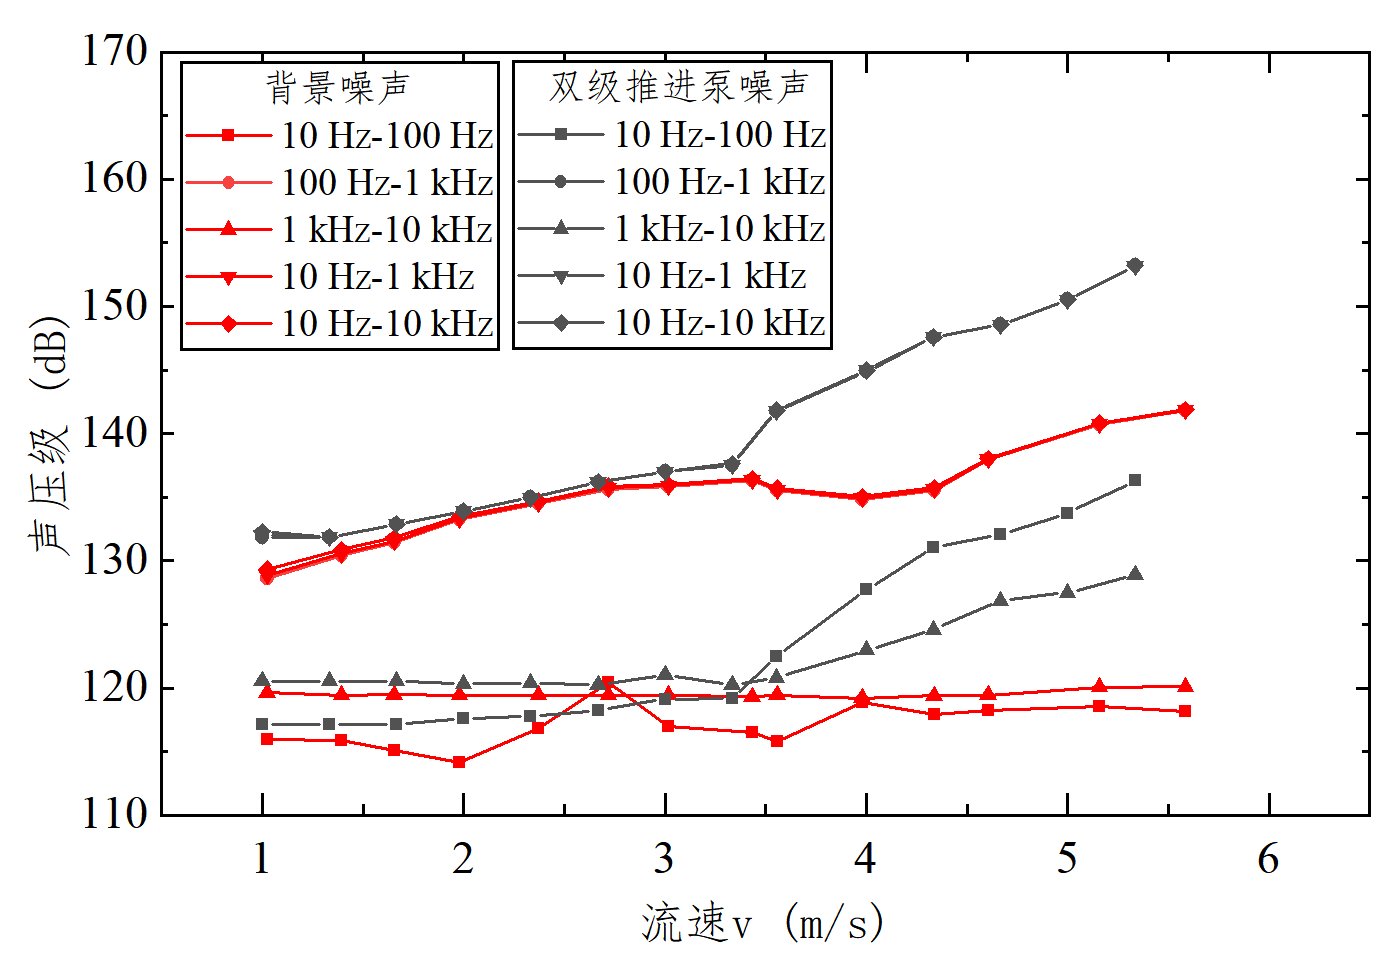
\includegraphics[scale=1]{3双级总声压级2.png}
    \caption{\label{fig:sjtotal}双级推进泵噪声在不同工况下各个频段的噪声总声压级}
\end{figure}

为了进一步评估流速对推进泵特征频段的影响,以及各个特征频段对噪声总级的贡献度。
基于噪声测试系统中的数据分析模块,获得了各测点不同频段的声压级平均值。
如\autoref{fig:sjtotal}所示为推进泵噪声在不同工况下噪声总声压级。
从图中可以看出,随着进速系数的变大,各个频段的声压级单调递增。
不同工况下中频段(100Hz-1kHz)、中低频段(10Hz-1kHz)和全频段(10Hz-10kHz)的变化曲线几乎重合,
这说明中低频段噪声是双级推进泵噪声最主要的贡献量。
对比水洞背景噪声的特征频段分析,
可以发现在低流速工况时,推进泵的噪声总声压级和背景噪声相近,
说明此时推进泵噪声信号信噪比低。
当流速从1.26m/s增大到5.05m/s时,背景噪声的声压总级增幅为7.2dB,推进泵声压总级的增幅为19.9dB。

在考虑背景噪声影响的基础上,推进泵噪声的总声压量级仍然会随流速的增大而增大。
此外,流速的增大不仅对全频段的声压级有增强作用,
还会提升推进泵噪声低中高三个频段的能量。
在流速变化的过程中,噪声总声压级幅值的增长速率发生了由慢变快的变化,
%当水速达到3.4m/s以后,噪声总声压级幅值的增长速率开始明显变大。
其中,流速的变化对低频段(10Hz-100Hz)和高频段(1kHz-10kHz)的总声压级影响较小,
当水速从1.26m/s增大到5.05m/s时,
低频段和高频段的总声压级的增幅分别为8.4dB和9.1dB。
水速对中频段(100Hz-1kHz)的总声压级影响更为显著,当水速从1.26m/s增大到5.05m/s时,
中频段的总声压级增幅达到12.6dB。
\subsubsection{双级推进泵噪声频谱分析}
随机选取了3号测点各工况下的噪声信号进行频谱分析,由上小节分析可知噪声频谱能量波动主要集中在中低频段,
因此本文重点讨论1500Hz以内的频谱特征。
分析结果中对频率作了无量纲化处理,即采用轴系转速进行无量纲化($f/f_n$)。
为了更好的表述频谱中的特征频率,
将双级推进泵的轴频定义为APF(对应$f_n$),首级叶轮叶频定义为BPF$_1$(对应5$f_n$),导叶叶频表示为SBPF(对应11$f_n$),
次级叶轮叶频定义为BPF$_2$(对应6$f_n$)。
\begin{figure}[htbp]
    \centering
    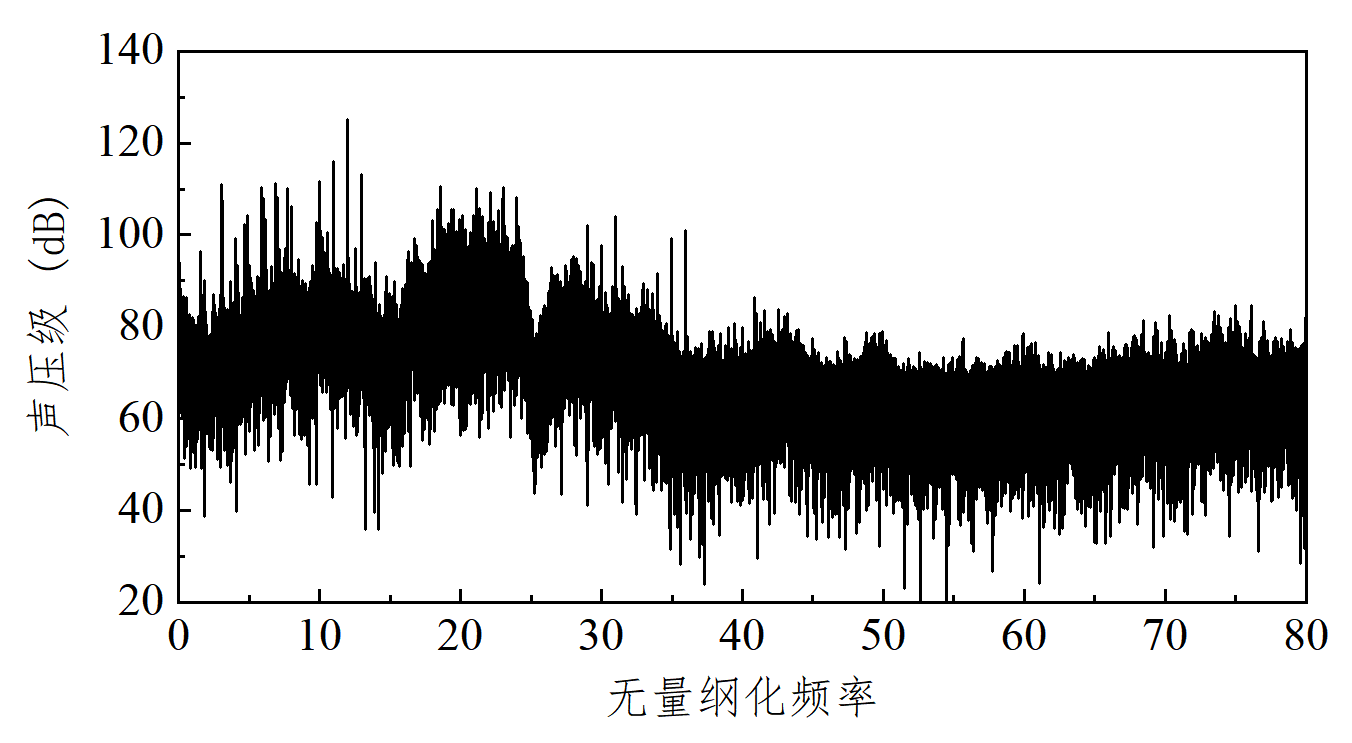
\includegraphics[scale=1]{3sj0.5频谱1.png}
    \caption{\label{fig:sj0.5}J=0.5工况下双级推进泵噪声频谱}
\end{figure}
\begin{figure}[htbp]
    \centering
    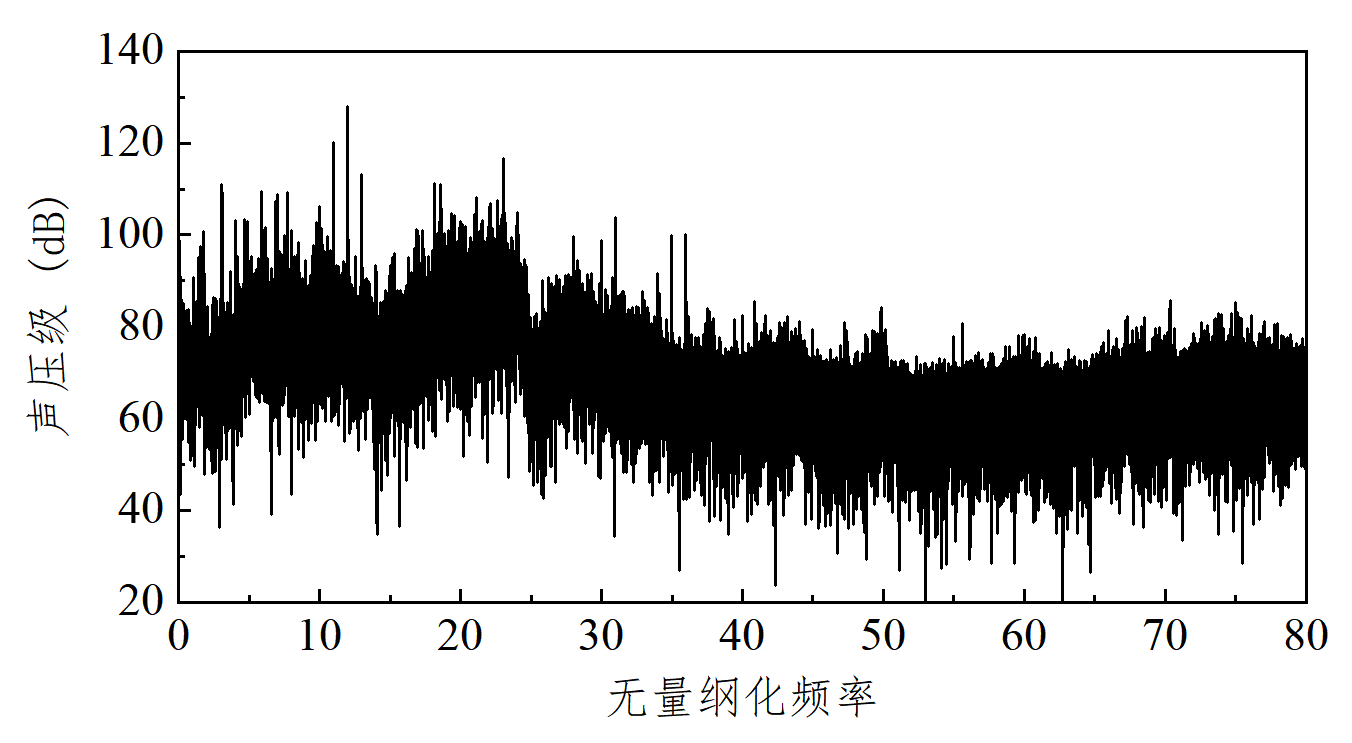
\includegraphics[scale=1]{3sj0.8频谱1.png}
    \caption{\label{fig:sj0.8}J=0.8工况下双级推进泵噪声频谱}
\end{figure}
\begin{figure}[htbp]
    \centering
    \includegraphics[scale=1]{3sj1.0频谱1.png}
    \caption{\label{fig:sj1.0}J=1.0工况下双级推进泵噪声频谱}
\end{figure}
\begin{figure}[htbp]
    \centering
    \includegraphics[scale=1]{3sj1.3频谱1.png}
    \caption{\label{fig:sj1.3}J=1.3工况下双级推进泵噪声频谱}
\end{figure}
\begin{figure}[htbp]
    \centering
    \includegraphics[scale=1]{3sj1.5频谱1.png}
    \caption{\label{fig:sj1.5}J=1.5工况下双级推进泵噪声频谱}
\end{figure}

如\autoref{fig:dj0.4},\autoref{fig:dj0.6},
\autoref{fig:dj0.79},\autoref{fig:dj1},\autoref{fig:dj1.2}所示,
分别为在不同工况下双级推进泵噪声的频谱图。
可以看出频谱中线谱成分丰富,推进泵噪声频谱特性表现为中低频宽带与线
谱噪声交叠和高频宽带的形貌。
随着流速的增大,频谱中中低频段的线谱和宽带幅值量级也在提升。
结合\autoref{fig:sjotc1}-\autoref{fig:sjotc4}双级推进泵噪声三分之一倍频程的分析,
这说明中低频线谱和宽带噪声对推进泵噪声都有非常明显的贡献。
中低频线谱和宽带成分也影响着频谱能量的分布。

在中低频段,比较明显的线谱有BPF$_1$,BPF$_2$,2BPF$_1$,2BPF$_2$,23ABF,SBPF,3BPF$_1$,7BPF$_1$,
其中2BPF$_1$,2BPF$_2$,SBPF线谱的幅值最为突出。
在APF-40APF之间还存在以APF为间隔的连续线谱成分,如4APF,7APF,8APF等较为突出的线谱。
除了这些特征线谱外,中低频段还存在很多幅值不显著的复杂线谱成分,
其中也包括背景噪声带来的干扰频率成分。

此外,在中低频段频谱中识别不到轴频APF成分,但是能观察到2ABF线谱成分。
在流速较小的工况下,噪声信噪比较低,2BPF$_1$,2BPF$_2$,SBPF等特征频率与其周围线谱的幅值差值不明显,不能准确且快速的被识别出来。
这些特征线谱随着流速的增大,在频谱中越容易被识别出来。

综上,双级推进泵噪声频谱特性表现为中低频宽带与线
谱噪声交叠和高频宽带的形貌,其噪声频谱具有较好的平稳性。
噪声能量主要集中在中低频段,中低频线谱和宽带噪声对推进泵噪声总声压级有明显贡献。
噪声的中低频段、高频段和全频段总声压级都随着流速的增大而增大,流速对推进泵噪声能量分布和声压量级的影响主要体现在中低频段。
频谱中线谱成分丰富,体现出轴频和叶频的谐波成分,
但是这些特征频率在频谱中不能准确且快速的被识别。

\section{本章小结}
本章以紧凑型前置导叶的单级推进泵和新型结构的双级推进泵为研究对象,
在大型空泡水洞中对其分别开展了噪声试验研究,
基于采集与分析系统的信号分析模块对试验数据进行了分析,
研究不同工况下推进泵噪声的声纹特征变化,
以及流速等与噪声的声学关联性。
本章主要内容包括以下几个方面:

(1)水洞背景噪声的试验研究和声纹特征分析。
由于水洞测试的局限性会影响推进泵中低频段声压级量级的可靠性,导致监测到的推进泵噪声的信噪比偏低。
本研究对多工况下的水洞背景噪声进行了试验及分析,分析表明背景噪声的能量主要集中中低频段,
对推进泵噪声的影响体现在中低频段。

(2)单级推进泵噪声的试验研究和声纹特征分析。
单级推进泵噪声频谱特性表现为中低频线谱噪声、中低频宽带噪声和高频宽带噪声。
噪声能量主要集中在中低频段,中低频线谱影响着噪声能量的分布,对推进泵噪声总声压级有显著贡献。
频谱中线谱成分丰富,
体现出轴频和叶频的谐波成分,
但是这些低频线谱特征在频谱中不能准确且快速的被识别。
噪声中低频段、高频段和全频段的总声压级随着流速的增大而增大,流速变化对推进泵噪声高频段的能量分布和总声压级影响较小,
对中低频段的能量分布和总声压级影响更加明显。

(3)双级推进泵噪声的试验研究和声纹特征分析。
双级推进泵噪声频谱特性表现为中低频宽带与线
谱噪声交叠和高频宽带的形貌,其噪声频谱具有较好的平稳性。
噪声能量主要集中在中低频段,中低频线谱和宽带噪声对推进泵噪声总声压级有明显贡献。
噪声的中低频段、高频段和全频段总声压级都随着流速的增大而增大,流速对推进泵噪声能量分布和声压量级的影响主要体现在中低频段。
频谱中线谱成分丰富,体现出轴频和叶频的谐波成分,
但是这些特征频率在频谱中不能准确且快速的被识别。

\chapter{推进泵噪声信号的特性研究}
\section{引言}
推进泵噪声频谱特性表现为中低频宽带与线
谱噪声交叠的形貌。频谱中线谱成分丰富,不仅包含有转子叶片
的离散线谱信息,同时也包括动静相互作用的影响。
但是由于水洞测试的局限性,
监测系统接收到的推进泵噪声信号的信噪比较低。
传统的噪声特征提取方法,如频谱分析等,具有抗噪性
能较差,难以提取弱信号特征等缺点,无法实现噪声信号中特征线谱的准确识别。
本章基于推进泵噪声信号的特性,结合其噪声信号产生的机理,对噪声信号进行
组分分析,进行噪声信号的建模仿真,验证循环平稳分析方法的抗噪性和提取能力。
\begin{comment}
推进泵噪声按声源类型的不同,可以将推进泵噪声分为流致噪声和振动噪声,其中流致噪声是推进泵噪声的主要贡献者。
流致噪声是由泵内非定常流动与泵相互作用产生的非定常流致激励所引起的,
前期研究发现,推进泵叶轮与其他部件之间的动静干涉是重要的流致噪声激励源。
动静干涉是指由于推进泵转子(如叶轮)和静止部件(如导叶和导管)之间的周
向不均匀流动在旋转过程中相互作用,从而导致了泵内部流道中复杂的非定常流动现象。
因此,推进泵噪声是推进泵流致激励特性的最直接的外在表现,
构建推进泵流致激励源特征提取的有效方法和途径,从噪声信号中分析出流致激励源
的影响程度以及两者的作用机理,对于推进泵低噪声设计及发展噪声能量主动控制技术至关重要。

第三章推进泵噪声试验结果显示,监测到的推进泵噪声频谱特性表现为中低频线谱噪声,中低频宽带谱噪声和
高频宽带谱噪声。
噪声信号中蕴含着丰富的流致激励源信息,但是难以从噪声信号频谱中提取出流致激励源特征信号,信号中存在复杂的干扰因素:
其一,推进泵处在复杂的背景环境声场中,背景声场中存在复杂的干扰
成分,影响测试系统对推进泵目标真实辐射噪声信号的监测;其二,推进泵结构复杂,
由于具有周期性分布的旋转、静止构件和导管,
辐射噪声的声源构件并不单一,其辐射噪声具有分量复杂性。
基于上述干扰因素,监测系统接收到的目标声场信号的
信噪比较低,特征信号如动静干涉频率、轴频等与其他背景噪声相比均较为微弱,给基于传统噪声特征提取方法带来了困难,
难以准确的获得推进泵的工作状态和结构信息,也给流致激励源特征的提取带来很大的难度。

其次,推进泵流致噪声存在显著的调制现象,上章节所研究的推进泵噪声频谱已呈现出较强的调制特性,
调制现象也是流致激励作用的结果,其中蕴含着丰富的流致激励源信息,
但是传统的频谱分析及解调方法无法实现高精度低频调制特征的提取。
因此,针对推进泵噪声信号的特点,开展对其噪声信号的分量分析研究,
基于其信号的循环平稳特性,
建立流致激励源-噪声信号模型,
探索合适的流致激励源特征提取方法,对噪声的机理分析和流致激励源特征提取有重要意义。
\end{comment}

\section{推进泵噪声信号分量分析}
推进泵由于其具有运转模式的周期性,具有明显的调制特性。
从信号组成成分来看,推进泵噪声信号成分主要包括确定性信号分量、调制信号分量和环境噪声信号分量。
确定性信号分量是由于非均匀流场与推进泵相互作用产生非定常负载、转子质量不平衡、不对中、电磁干扰等因素引起的,
在稳态工况下其具有一阶的统计特性;
调制信号分量是由于推进泵周期性旋转构件在旋转过程中产生周期性冲击作用引起的,
最终辐射产生调制噪声信号,其具有二阶的统计特性;
环境噪声信号分量主要由于推进泵的噪声测试环境和监测系统引入的
环境干扰噪声信号,该噪声信号一般为高斯白噪声,不具有一阶、二阶及高阶的统计周期性\cite{antoniCyclostationaryModellingRotating2004a,song2019}。
\begin{comment}
推进泵噪声信号模型可以利用\autoref{fig:signal_modle}进行表示。
\begin{figure}[htbp]
    \centering
    \includegraphics[scale=0.5]{5推进泵信号模型.png}
    \caption{\label{fig:signal_modle}推进泵噪声信号模型}
\end{figure}
\end{comment}

\subsection{确定性信号分量}
确定性信号分量是由于非均匀流场与推进泵相互作用产生非定常负载、转子质量不平衡、不对中等因素引起的,
其随时间具有确定的函数关系。确定性信号分量的特点为,其信号模型可以利用函数模型进行准确表征,
在稳态工况下其具有一阶的统计特性,一阶统计特性可以表示为\autoref{equ:one}所示。
\begin{equation}
    \label{equ:one}
    m_{x}\left ( t \right ) =E\left [ x_{d}\left ( t   \right )  \right ]
\end{equation}

式中$E[*]$表示信号的统计平均函数,
在稳态工况下,推进泵确定性信号成分的一阶矩满足\autoref{equ:one1}。
\begin{equation}
    \label{equ:one1}
    m_{x}\left ( t \right ) =m_{x}\left ( t+T_d \right )
\end{equation}

式中$T_{d}$表示信号的时间周期,该分量在进行信号的一阶统计分析
时,信号的特征频率及幅值并不会发生显著变化。
\subsection{调制信号分量}
调制信号分量主要为推进泵旋转构件在旋转过程中产生周期性冲击作用,
各频率信号相互调制,最终辐射产生调制噪声信号。该组分具有二阶的统计特性,
二阶统计特性可以表示为\autoref{equ:two}所示。
\begin{equation}
    \label{equ:two}
    m_{2x}\left ( t, \tau \right )  =E\left [ x_{m}\left ( t \right ) \ x_{m}\left ( t+\tau \right )  \right ] 
\end{equation}

式中$\tau$表示延迟时间。
在稳态工况下,对于调幅调制信号其二阶统计量具有稳定的周期性如\autoref{equ:two1}所示,
该信号分量统计特征参量随时间呈现出周期性的变化规律。
\begin{equation}
    \label{equ:two1}
    m_{2x}\left ( t, \tau \right )  =m_{2x}\left ( t+T_m, \tau \right )
\end{equation}

式中$T_m$表示水力旋转机械监测信号二阶统计量的循环周期。
并且二阶统计量的周期与调制信号的特征频率之间存在倒数关系如\autoref{equ:two2}所示,
\begin{equation}
    \label{equ:two2}
    \alpha =\frac{1}{T_{m} } 
\end{equation}

式中$\alpha$表示调制信号分量的调制频率。
推进泵噪声信号中的调制信号分量
包含着丰富的流场信息和运行状态,利用推进泵调制信号分量的二阶统计特性
能够准确的获得其调制周期,是进行推进泵调制线谱特征提取的有效手段。
\subsection{环境噪声信号分量}
环境噪声信号分量主要由于推进泵的噪声测试环境和监测系统引入的
环境干扰噪声信号。该噪声信号一般为高斯白噪声,不具有一阶、二阶及高阶的统计周期性。
因此利用信号的统计特性,能够有效的实现监测信号中噪声信号分量的消除,
有助于推进泵特征频率的提取。

\section{循环平稳统计量}
推进泵周期运转的方式使其噪声信号具有周期特性,同时由于实际运转状态存在很多随机因素,
从而使得其噪声信号兼顾周期性和随机性的特点,因此推进泵噪声信号可以归于循环平稳的范畴。
循环平稳信号在当今的工业生产中普遍存在于通讯、旋转机械等应用场景,
近年来循环平稳分析方法开始用于机械故障检测以及旋转机械信号特征提取领域。
\subsection{一阶循环平稳统计量}
%William A. Gardner定义信号的一阶周期性为信号并不需要非线性变换而本身就包含有限强度的加性正弦波,
一阶循环平稳也被称为一阶周期性,这类信号采用传统的频谱分析也可以进行有效分析。
对一阶周期性信号作统计平均求其均值,则其均值为时间的函数,通常称之
为时变均值,即一阶时变矩。由于该均值为时间的函数,无法直接使用时间平均来估
计信号的均值\cite{zhou2006}。但是,由于该信号的周期$T_{0}$可以通过先验知识得到,就可以对该信号
以$T_{0}$为周期进行采样,且满足遍历性,从而可以用样本平均来代替其均值,
时变均值的定义如\autoref{equ:yijie}所示:

\begin{equation}
    \label{equ:yijie}
    m_{1x} \left ( t \right ) =\lim_{x \to \infty} \frac{1}{2N+1}\sum_{n=-N}^{N}x\left ( t+nT_{0}  \right )   
\end{equation}

式中$m_{1x}$表示时域平均信号,$2N+1$表示平均的次数,$T_{0}$表示平均数据周期。
若令对时变$m/T_{0} =\alpha$,并对均值作Fourier级数展开,
可得到时变均值的$\alpha$频率分量$M_{1x}^{\alpha}$称为循环均值。

根据时变均值的定义式可以看出,该公式其实就是传统信号分析处理
中的时域同步平均算法,不具备将调制信号从载波信号中解调出来的能力。
同步平均在一定程度上有抑制噪声的作用,同时也会削弱原始信号的能量。
在实际运用中,确定性信号分量的
特征提取需要对时域信号的分辨率具有一定的要求,
为了得到良好的确定性信号分量和降噪效果,
平均信号的平均次数$2N+1$需要尽量的大,这对监测信号的数据长度要求比较高\cite{陈进2013机械故障特征提取的循环平稳理论及方法}。

在使用时域平均算法对推进泵信号确定性成分进行提取时,
处理后的信号波形虽然能降低噪声干扰,但是推进泵噪声的确定性信号成分复杂,
难以实现特征线谱的准确识别。
因此在本文后续的研究,将采用该算法作为信号降噪的预处理手段。

\subsection{二阶循环平稳统计量}
根据现有的旋转机械循环平稳理论的分析和研究基础,推进泵产生的辐
射噪声信号的二阶累积量函数具有一定的周期性,称为二阶循环平稳信号。
本文主要将二阶循环统计量作为切入点,对推进泵辐射噪声信号进行解调分析和特征频率提取。
常用循环平稳分析算法的解调谱有相关谱、相干谱、增强包络谱等,本文将采用相干谱对推进泵噪声信号
进行解调分析。
首先,本文所采用的二阶循环统计量引入了时变自相关函数,
见\autoref{equ:erjie}。 
\begin{equation}
    \label{equ:erjie}
    R_{x} \left ( t,\tau  \right ) =\lim_{x \to \infty} \frac{1}{2N+1} \sum_{n=-N}^{N} x\left ( t+nT_0+\frac{\tau }{2}  \right )x^{\ast }\left ( t+nT_0-\frac{\tau }{2}  \right )=R_{x}\left ( t+T_0,\tau  \right )    
\end{equation}

式中,$T_0$和$\tau$表示为周期以及滞后时间。
循环自相关函数由自相关函数展开成傅立叶级数后得到,如\autoref{equ:erjie1}所示。
\begin{equation}
    \label{equ:erjie1}
    R_{\alpha }^{x} \left ( \tau  \right ) =\lim_{x \to \infty} \frac{1}{T}\int_{T}^{}x\left ( t+\frac{\tau }{2}  \right )x^{\ast } \left ( t-\frac{\tau }{2} \right ) e^{-j2\pi \alpha t} dt   
\end{equation}

式中$\alpha$表示循环频率,它的倒数即为循环周期,$j$表示虚数单位。

通过对循环自相关函数进行傅里叶变换可得到谱相关密度函数,见\autoref{equ:erjie2}所示。
\begin{equation}
    \label{equ:erjie2}
    SC_{\alpha }^{x} \left ( f  \right ) =\int_{-\infty }^{\infty } R_{\alpha }^{x}\left ( \tau  \right )  e^{-j2\pi f t} d\tau   
\end{equation}

然而在循环密度谱的应用中,一些相对微弱的振动特征会被谱的尺度效
应所淹没。因此,将循环密度谱作了归一化处理,称为循环谱相关性,
有效检测出微弱的振动信号特征,揭示振动信号循环平稳性的强弱\cite{li2018}。
循环谱相干性如\autoref{equ:erjie3}所示。
\begin{equation}
    \label{equ:erjie3}
    \gamma _{x}^{\alpha}\left ( f \right ) =\frac{corr_{x}\left ( f+\frac{\alpha }{2}, f-\frac{\alpha }{2} \right )  }{\sqrt{P_{x}\left ( f+\frac{\alpha }{2} \right )P_{x}\left ( f-\frac{\alpha }{2} \right ) } } =\frac{SC_{x}^{\alpha }\left ( f \right )  }{\sqrt{SC_{x}^{0} \left ( f+\frac{\alpha }{2} \right )SC_{x}^{0} \left ( f-\frac{\alpha }{2} \right )} }  
\end{equation}

\section{推进泵噪声信号的建模与仿真分析}
\subsection{推进泵噪声信号的调幅调制模型}
监测的噪声信号为水力旋转机械的三种信号分量与传递路径函数卷积的结果,其噪声信号模型如\autoref{equ:component}所示。 
\begin{equation}
    \label{equ:component}
    x\left ( t \right ) =\left ( x_d\left ( t \right )+x_m\left ( t \right )+x_e\left ( t \right ) \right )\ast h 
\end{equation}

式中,$x\left ( t \right )$表示噪声信号,
$x_d\left ( t \right )$为噪声信号中的确定性信号分量,
$x_m\left ( t \right )$为噪声信号中的调制信号分量,
$x_e\left ( t \right )$为噪声信号中的的环境噪声分量,$\ast$表示卷积运算,
$h$表示噪声激励源到监测点之间的传递函数。 
推进泵试验中的振动传递系统可以视为线性时不变系统,
在实际信号中,传递函数只是对信号幅值有一定
的影响,但是对信号的频率特征影响较小,因此在后续的研究中忽略传递函数对监测信号
的影响\cite{song2019}。 

根据推进泵不同的工作状态,其调制信号可以分为稳态工况下的
调幅信号和非稳态工况下的调幅-调频信号,两种工况分别针对匀速运转和变速运转两种
状态。本文只考虑推进泵匀速运转的状态,相关试验也是在匀速工况下开展,
因此文中将对稳态工况下的调幅调制信号的调制模型进行建模与分析。 
稳态工况下,由于推进泵的运转速度保持不变,因此冲击力的作用周期保持不变,
最终使得调幅调制信号的特征调制频率保持稳定不变。

推进泵的噪声情况是动叶、静叶和导管等构件与非均匀流场相互作用的综合结果,
第三章推进泵噪声试验结果显示,监测到的推进泵噪声频谱特性表现为中低频宽带线谱噪声和高频宽带谱噪声。
根据其特点将其构建成具有线谱载波和宽带载波,多组分调制频率的调幅调制信号\cite{Tarkan2013PREDICTION}。
信号调幅调制模型如\autoref{equ:tiaozhi}所示。
\begin{equation}
    \label{equ:tiaozhi}
    x\left ( t \right ) =\sum_{i=1}^{k}\left [ A_{i}\cos \left ( 2\pi f_{m,i}t  \right )\left ( B_{i}\cos\left ( 2\pi f_{c,i}t  \right )   \right )+D_{i}\cos\left ( 2\pi f_{n,i}t  \right )v\left ( t \right )      \right ]  
\end{equation}

式中,$A_i$为线谱载波的调制信号的幅值,$f_{m,i}$为调制信号的调制频率,$f_{c,i}$为线谱载波信号的载波频率,
$B_i$为载波信号的幅值,$v\left ( t \right )$为随机平稳信号,$D_i$为随机平稳信号的调制信号的幅值,
$f_{n,i}$为随机平稳信号的调制信号的调制频率。
\subsection{仿真信号研究}
在运用循环平稳分析手段处理推进泵噪声信号之前,
为了验证循环平稳解调算法提取多组分调制频率的有效性和良好的抗噪性能,仿真分析是一种非常有效的方式。
基于推进泵噪声监测信号各组分的特点,该仿真信号的载波信号包含线谱载波、宽带载波两部分,
与实际的推进泵调制信号特征相对应,本文所建立的仿真模型如\autoref{equ:fangzhen}所示。 
\begin{equation}
    \label{equ:fangzhen}
    x\left ( t \right ) =\sum_{i=1}^{2}\left [ A_{i}\cos \left ( 2\pi f_{m,i}t  \right )\left ( B_{i}\cos\left ( 2\pi f_{c,i}t  \right )   \right )+D_{i}\cos\left ( 2\pi f_{n,i}t  \right )v\left ( t \right )      \right ]  
\end{equation}

式中,$f_{m,i}=$17Hz,27Hz表示线谱载波的调制信号频率,$f_{n,i}=$37Hz,47Hz表示宽带载波的调制信号频率,
$f_{c,i}=$1000Hz,2000Hz表示线谱载波信号频率,$A_i=$1,1为线谱载波的调制信号的幅值,
$B_i$=1,1为线谱载波信号的幅值,
$D_i$=1,1为随机平稳信号的调制信号的幅值,
$v\left ( t \right )$为随机平稳信号。

对该仿真信号进行二阶循环平稳统计量分析,代入\autoref{equ:erjie3}可推导出循环谱相干性的理论值。
由分析结果可知,
该仿真信号的循环相干谱当循环频率等于以下四种情况的时候,循环相干谱出现非零值:
(1)当$\alpha=0$时,循环密度谱则退化成为一般的功率谱密度;
(2)调制频率;
(3)调制频率的谐频;
(4)干涉频率。

因此,当一个存在多调制信号的幅值调制信号经过循环密度谱处理
后,除了得到想要的调制频率之外,其调制频率的谐频以及其干涉频率均会出现。
但是调制频率处的幅值会高于其谐频和干涉频率成分处的幅值,可通过这一特点从循环相干性谱图中出现的
若干特征线谱中区分出调制频率。
对于该仿真信号来说,其循环相干性谱图上除了出现四个调制频率(17Hz,27Hz,37Hz,47Hz)的线谱,
还会出现这四个调制频率的谐频成分,以及调制频率的干涉频率(10Hz,44Hz等)。

为了验证循环平稳解调算法提取多组分调制频率的有效性和良好的抗噪性能,
在信号模型中分别加入不同程度的高斯白噪声,仿真信号的信噪比(Signal to Noise 
Ratio,SNR)分别为0dB,-5dB,-10dB。由于循环谱相干性能表示调制信号的调制强度影响,
因此本文以循环谱相干性的结果讨论为主。
仿真信号的循环谱相干性采用一种快速算法计算\cite{antoniFastComputationSpectral2017}。信号的采样
频率设置为20480Hz,
不同信噪比的仿真信号的循环谱相干性分析结果如\autoref{fig:db0}、\autoref{fig:db-5}
和\autoref{fig:db-10}所示。
\begin{figure}[htbp]
    \centering
    \includegraphics[scale=1]{origindb01.png}
    \caption{\label{fig:db0}SNR=0dB循环平稳解调分析结果}
\end{figure}

当 SNR=0dB时,循环平稳算法能很好的表征调制特征频率。如\autoref{fig:db0}所示,在循环谱相干性图上出现若干条特征谱线,
包括四个调制频率(17Hz,27Hz,37Hz,47Hz)的谱线,
四个调制频率的谐频成分(34Hz,54Hz,74Hz,94Hz等),以及调制频率的干涉频率10Hz和44Hz等。
其中调制频率处的平均相干系数幅值均大于其谐频和干涉频率成分处的循环相干系数。
\begin{figure}[htbp]
    \centering
    \includegraphics[scale=1]{origindb-5.png}
    \caption{\label{fig:db-5}SNR= -5dB循环平稳解调分析结果}
\end{figure}

当SNR=-5dB时,原始信号中包含的宽带调制信号组分和高斯白噪声信号组成的噪声
组分较多,信号的信噪比较低。如\autoref{fig:db-5}所示,在循环谱相干性图上出现若干条特征谱线,
通过特征频率处的幅值大小可以判断出调制频率,
此时循环平稳算法依然能够进行低频特征频率的表征。

\begin{figure}[htbp]
    \centering
    \includegraphics[scale=1]{origindb-10.png}
    \caption{\label{fig:db-10}SNR= -10dB循环平稳解调分析结果}
\end{figure}

当SNR=-10dB时,原始信号中噪声成分非常高。当仿真信号的信噪比
降低时,如\autoref{fig:db-10}所示,虽然循环谱相干性图中出现了若干干扰频率,
但是解调谱上显著体现出四个调制频率的特征谱线,
该方法依然可以获得比较好的低频特征频率的解调效果,体现出较高的
解调精度和抗噪性能。

进了进一步验证信噪比大小对仿真结果的影响,在循环谱相干性的仿真测试中
对比了不同信噪比对仿真结果的影响,如\autoref{equ:fangzhen1}所示。该仿真信号
仍为一个幅值调制信号,只设置了一个调制信号,其相应的调制频率设为10Hz。
根据理论预测,除了在调制频率处,在二阶谐频20Hz处也会产生非零的特征谱线。
\begin{equation}
    \label{equ:fangzhen1}
    x\left ( t \right ) =\left ( 1+\cos \left ( 2\pi f_mt \right )  \right ) v\left ( t \right ) 
\end{equation}

式中$v\left ( t \right )$为随机平稳信号,$f_m$=10Hz为载波信号的调制频率。

\autoref{fig:SNR}对比了在这两个特征频率处的平均相干系数在不同信噪比下的结果,可见
平均相干系数会随着信噪比的减小而衰减,信噪比并不影响判断两个非零特征
谱的相对大小。

\begin{figure}[htbp]
    \centering
    \includegraphics[scale=0.85]{4仿真信噪比.png}
    \caption{\label{fig:SNR}信噪比对平均相干系数的影响
    }
\end{figure}

综上,通过多组分调制信号和载波信号的解调仿真实验,
验证了循环平稳算法能识别宽带载波和线谱载波的多组分调制频带,
表现出较高的提取精度以及抗噪性能。
\section{本章小结}
本章基于推进泵噪声信号的特点,结合其噪声信号产生的机理,
对噪声信号进行了组分分析、循环平稳特性、调制模型的研究,
为推进泵低信噪比噪声信号的特征线谱提取和调制特性分析奠定了理论基础。
本章主要内容包括以下几个方面:

(1)推进泵噪声信号的组分分析。结合推进泵噪声信号产生的机理,将推进泵噪声信号分量分为
确定性信号分量、调制信号分量和噪声信号分量。
确定性信号分量具有一阶的统计特性,调制信号分量具有二阶的统计特性,噪声信号分量不具有统计特性,
根据各组分的统计特性能够实现推进泵信号特征的初步提取。 

(2)推进泵噪声信号的循环平稳特性分析。
基于推进泵噪声信号的循环平稳特性,对一阶循环平稳统计量和二阶循环平稳统
计量进行了介绍,
为噪声信号的预处理和调制信号的解调算法提供基础。
%为循环平稳分析方法在噪声信号中的应用奠定了理论基础。

(3)推进泵噪声信号的建模与仿真分析。
结合推进泵噪声信号产生的机理和噪声信号特征,对匀速运转工况下的噪声
信号建立了幅值调制信号模型。采用循环谱相干性作为二阶循环平稳统
计量对噪声信号的仿真模型进行了研究,验证循环平稳解调算法提
取多组分调制频率的有效性和良好的抗噪性能。


\chapter{推进泵噪声的特征线谱提取和分析}
\section{引言}
由经典声学理论可知,脉动力源远场辐射噪声的声压表达式为
\begin{equation}
    \label{equ:p}
    p\left ( \mathbf{r} ,t \right ) =\frac{\mathbf{F}\cdot \mathbf{r} }{4\pi rc} =\frac{F\left ( t' \right ) }{4\pi rc}\cos \theta  
\end{equation}
式中,$t'$为迟滞时间,$\mathbf{F}$为脉动力,$r$为脉动力源到测点距离,$\theta$为与矢量之间夹角,
$\cos \theta$项用于表征脉动力源的偶极声场指向性,该式表明了脉动力源与其辐射声场之间的直接联系\cite{__2016杨琼方}。
推进泵导叶、叶轮和导管壁面的非定常脉动压力是推进泵无空化状态下最主要的低频线谱噪声源。
%说明非定常脉动力的特征线谱频率能在噪声信号中体现出来。
在推进泵噪声预报方面,往往也是通过CFD计算得出的推进泵壁面压力脉动及轴向脉动推力,
从而分析推进泵低频离散线谱。

%由于推进泵低频线谱噪声的提取面临环境干扰强、直接测量难度大的问题,
%因此本章CFD数值模拟来验证验证循环平稳分析方法提取特征线谱的可行性,
在上节循环平稳对多调制信号模型的解调分析中,分析结果中有调制频率的干涉项产生。
因此在使用循环平稳分析推进泵噪声信号之前,需要通过数值模拟获取特征频率的先验知识。
本章通过CFD数值模拟计算获取了多工况下推进泵的激励力信号,
分析了推进泵脉动力源的关键特性,获取了特征频率的先验知识。
其次,引入二阶循环统计量提取了试验噪声信
号中的特征线谱。最后联合数值模拟中获得的非定常脉动力特征,验证了循环平稳分析
方法提取特征线谱的可行性,分析了推进泵噪声的调制特性。

\begin{comment}
    
推进泵噪声是推进泵流致激励特性的最直接的外在表现,
推进泵噪声信号中包含着丰富的运行状态和流致激励源特性,
前面章节的研究表明推进泵噪声的频谱呈现出宽带与线谱交叠的形貌,中低频线谱成分复杂,
噪声信噪比较低,特征信号如流致激励源特征频率、轴频等与其他背景噪声相比均较为微弱,
给基于传统噪声特征提取方法带来了困难,难以准确的获得推进泵的工作状态和结构信息。
上章节通过对噪声的成分分析,基于推进泵噪声的循环平稳特征,推导出流致激励源-噪声信号的幅值调制模型。
进一步为了验证从噪声信号中提取流致激励源特征的合理性和可行性,
本章节通过非定常数值模拟计算获取了多工况下推进泵的激励力信号,
分析了推进泵流致振动噪声源的关键特性,
采用循环平稳分析方法实现推进泵低频特征的提取,
联合从噪声信号中提取特征频率的结果与流致激励源的模拟结果,
从噪声信号中分析出流致激励源对噪声的影响程度以及两者的作用机理,
探究推进泵噪声的调制特性。
\end{comment}
\section{单级推进泵的特征线谱提取和分析}
\subsection{数值模型及计算方法}
为了验证循环平稳分析方法提取噪声中特征线谱的可行性,本章节首先对脉动力源的关键特性进行了分析,
获取了特征频率的先验知识。
本文对单级推进泵开展了非定常数值模拟计算,以获得推进泵内部的脉动力特征。
数值模拟计算依托商用平台ANSYS Fluent开展,
采用CFX Turbogrid与ICEM生成计算域网格如\autoref{fig:djjisuanyu}所示。
为了尽可能减小水洞壁面效应对研究对象绕流和推进泵内部流动的影响,
计算域总体呈圆柱形,长16L、直径10D\cite{jiang2017}。其中,L为推进泵轴向长度,
D为叶轮直径。计算域入口距离推进泵前缘5L,
设置为速度入口条件;计算域出口距离推进泵后缘10L,设置为压力出口条件。
\begin{figure}[htbp]
    \centering
    \includegraphics[scale=1.4]{4推进泵计算域模型.png}
    \caption{\label{fig:djjisuanyu}计算域及边界条件}
\end{figure}

根据单级推进泵工作特点,将泵网格划分为旋转域与静止域,
相邻计算域采用interface连接,
外流域壁面和物面采用无滑移壁面条件。
泵内、外计算域均采用六面体结构化网格。
此外,在叶片、导管等壁面以及交界面的网格进行加密处理。
为了适应SST湍流模型,如\autoref{fig:djyplus}所示,使叶片表面y$^+$小于15,
以得到合理的边界层计算结果。
如\autoref{fig:djwangge}、\autoref{fig:djjisuanyuwangge}所示为单级推进泵网格和计算域网格。
\begin{figure}[htbp]
    \centering
    \subfigure[单级推进泵表面网格]{
    \includegraphics[scale=0.23]{5单级推进泵网格.png}
    }
    \subfigure[表面网格加密]{
    \includegraphics[scale=0.16]{5单级网格加密.png}
    }
    \caption{\label{fig:djwangge}单级推进泵表面网格}
\end{figure}
\begin{figure}[htbp]
    \centering
    \includegraphics[scale=1.0]{4计算域网格.png}
    \caption{\label{fig:djjisuanyuwangge}单级推进泵计算域网格}
\end{figure}
\begin{figure}[htbp]
    \centering
    \includegraphics[scale=1.0]{5单级yplus.png}
    \caption{\label{fig:djyplus}单级推进泵表面y$^+$}
\end{figure}
经过网格无关性验证后确定总网格量,各计算域网格数如\autoref{tab:djshuliang}所示。
\begin{table}[htbp]
    \centering
    \caption{\label{tab:djshuliang}单级推进泵各计算域网格数量}
    \begin{tabular}{ccccc}
        \toprule
        计算域 & 外流域 & 叶轮域 & 导叶域  & 网格总量 \\
        \midrule
        网格量 & 132万 & 122万 & 116万 & 370万 \\
        \bottomrule
    \end{tabular}
\end{table}

单级推进泵的CFD数值计算采用的湍流模型为SST k-ω模型,压力速度耦合方式为SIMPLEC,
压力项离散方式为二阶离散,动量项离散方式为二阶迎风格式,其他项均采用一阶迎风格式离散\cite{rao2012,bai2020}。
CFD数值计算结果与试验结果对比如\autoref{fig:sj_monishiyan}所示。
推力系数的试验值和模拟值基本吻合,效率和扭矩系数在小流量的情况下吻合较好,在大流量的情况下偏差较大。
总体来说,CFD仿真结果与实验数据呈现了较好的一致性,
验证了计算结果的可靠性。
\begin{figure}[htbp]
    \centering
    \includegraphics[scale=1]{5单级模拟试验对比.png}
    \caption{\label{fig:sj_monishiyan}单级推进泵敞水性能试验与CFD模拟结果对比}
\end{figure}

为获取推进泵的脉动力源特征,本文开展了非定常计算。
其中,非定常计算的时间步设为叶轮旋转一度所需的时间。
导叶与导管四个部件上轴向非定常力计算采用定长计算得到的结果
作为初始值以增强收敛性,并且每个非定常计算过程包含叶轮运转20圈的结果,
前3圈的数据由于计算还没有完全收敛而没有在进一步的分析中采用。
\subsection{非定常脉动力仿真结果与分析}
通过非定常模拟获得了叶轮、导叶与导管等部件上的轴向非定常脉动力,
分别计算了推进泵在进速系数分别为0.4,0.79试验工况下的数据。
分析结果中对频率作了无量纲化处理,即采用轴系转速进行无量纲化 ($f/f_n$)。为了更好的表述
频谱中的特征频率,将单级推进泵的轴频定义为 APF(对应$f_n$),叶轮叶频定义为 BPF
(对应 7$f_n$),导叶叶频表示为 SBPF(对应 11$f_n$)。
\begin{figure}[htbp]
    \centering
    \includegraphics[scale=1]{5单级非定常激励力0.4_1.png}
    \caption{\label{fig:djCFD0.4}J=0.4工况下单级推进泵轴向脉动力频谱}
\end{figure}

\autoref{fig:djCFD0.4}展示了J=0.4工况下,
单级推进泵叶轮、导叶与导管等部件上轴向非定常脉动力的频谱。
可以看出,导叶上轴向脉动力能量集中在2BPF线谱附近。
导管上的轴向脉动力以SBPF、BPF和2BPF最为突出。
叶轮上的脉动力除了BPF和SBPF等线谱特征外,还存在BPF-2APF和BPF+2APF等特征。
\autoref{fig:djCFD0.79}展示了J=0.79工况下的各构件上轴向脉动力频谱,
该工况下脉动力特征与J=0.4工况类似。
对于该单级推进泵的脉动力而言,
除了BPF、SBPF等离散线谱外,还存在有叶频与轴频之间的差值线谱频率。
\begin{figure}[htbp]
    \centering
    \includegraphics[scale=1]{5单级非定常激励力0.79_1.png}
    \caption{\label{fig:djCFD0.79}J=0.79工况下单级推进泵轴向脉动力频谱}
\end{figure}
\subsection{试验噪声的特征线谱提取与分析}
采用循环平稳分析方法对多个工况的推进泵试验噪声信号进行了低频特征解调分析,
进而提取单级推进泵的特征线谱。
\begin{figure}[htbp]
    \centering
    \includegraphics[scale=1]{dj1.2解调1.png}
    \caption{\label{fig:djjietiao1.2}J=0.4工况下单级推进泵噪声循环平稳分析结果}
\end{figure}

\begin{figure}[htbp]
    \centering
    \includegraphics[scale=1]{dj0.4解调2.png}
    \caption{\label{fig:djjietiao0.4}J=0.79工况下单级推进泵噪声循环平稳分析结果}
\end{figure}

\autoref{fig:djjietiao1.2}为J=0.4工况下单级推进泵噪声信号的循环谱相干性分析结果,
对循环频率进行了归一化处理,即采用轴系转速进行无量纲化 ($f/f_n$)。
从循环谱相干性图中可以清晰识别出APF,BPF等频率成分。
\autoref{fig:djjietiao0.4}展示了 J=0.79工况下单级推进泵噪声信号的分析结果。
除了APF,BPF,2BPF和3BPF等特征频率,还提取到SBPF等频率成分,
可以与脉动力中的低频离散线谱频率对应起来。
其中SBPF特征线谱的调制强度微弱,APF和BPF等特征频率表现出更明显的调制效应。
\autoref{fig:djjietiao0.79}展示了 J=1.2工况下单级推进泵噪声信号的循环谱相干性分析结果。
该工况下解调谱和J=0.4工况解调结果相似,轴频和动叶叶频的调制效应占主导。


\begin{figure}[htbp]
    \centering
    \includegraphics[scale=1]{dj0.79解调2.png}
    \caption{\label{fig:djjietiao0.79}J=1.2工况下单级推进泵噪声循环平稳分析结果}
\end{figure}

联合试验噪声信号的循环平稳分析和非定常脉动力的特征分析结果,
循环平稳分析方法提取出的低频线谱成分可以和非定常脉动力的特征线谱对应起来,
验证了循环平稳分析方法提取特征线谱的可行性。
相比第三章频谱分析的提取结果,循环平稳分析方法能更加清晰的识别出特征线谱。
通过对多工况下的不同信噪比信号进行特征提取,进一步验证了循环平稳分析方法的抗噪性。
以上的解调分析表明单级推进泵噪声信号具有强烈的调制特征,其中轴频和动叶叶频的为主要的调制频率。
随着流速的增大,动叶叶频的调制效应也愈发显著。

\section{双级推进泵的特征线谱提取和分析}
\subsection{数值模型及计算方法}
双级推进泵流场的数值模拟计算依托商用平台ANSYS Fluent开展,
采用CFX Turbogrid与ICEM生成计算域网格如\autoref{fig:jisuanyu}所示。
为了尽可能减小水洞壁面效应对研究对象绕流和推进泵内部流动的影响,
计算域总体呈圆柱形,长16L、直径10D;其中,L为推进泵轴向长度,
D为叶轮直径。计算域入口距离推进泵前缘5L,
设置为速度入口条件;计算域出口距离推进泵后缘10L,设置为压力出口条件。
\begin{figure}[htbp]
    \centering
    \includegraphics[scale=1.3]{4推进泵计算域模型.png}
    \caption{\label{fig:jisuanyu}计算域及边界条件}
\end{figure}
\begin{figure}[htbp]
    \centering
    \includegraphics[scale=1.2]{4表面网格.png}
    \caption{\label{fig:sjwangge}双级推进泵表面网格}
\end{figure}
\begin{figure}[htbp]
    \centering
    \includegraphics[scale=1.0]{4计算域网格.png}
    \caption{\label{fig:jisuanyuwangge}计算域体网格}
\end{figure}

根据双级推进泵的工作特点,将计算域分为:外流域、首级叶轮域、导叶域和次级叶轮域。
两级叶轮所在的是旋转域,其余的为静止域,两相邻的计算域采用interface连接。
外流域壁面和物面采用无滑移壁面条件。
为了适应SST湍流模型,如\autoref{fig:djyplus}所示,使叶片表面y$^+$小于30,导管表面y$^+$小于45,
以得到合理的边界层计算结果。
泵内、外计算域均采用六面体结构化网格,
如\autoref{fig:sjwangge}、\autoref{fig:jisuanyuwangge}所示为双级推进泵网格和计算域网格。
\begin{figure}[htbp]
    \centering
    \includegraphics[scale=1.0]{5双级yplus.png}
    \caption{\label{fig:djyplus}双级推进泵表面y$^+$}
\end{figure}

经过网格无关性验证后确定总网格量,各计算与网格数如\autoref{tab:sjshuliang}所示。
\begin{table}[htbp]
    \centering
    \caption{\label{tab:sjshuliang}双级推进泵各计算域网格数量}
    \begin{tabular}{cccccc}
        \toprule
        计算域 & 外流域 & 首级叶轮域 & 导叶域 & 次级叶轮域 & 网格总量 \\
        \midrule
        网格量 & 132万 & 95万 & 95万 & 101万 & 437万 \\
        \bottomrule
    \end{tabular}
\end{table}

双级推进泵的CFD数值计算采用的湍流模型为SST k-ω模型,压力速度耦合方式为SIMPLEC,
压力项离散方式为二阶离散,动量项离散方式为二阶迎风格式,其他项均采用一阶迎风格式离散。
CFD数值计算结果与试验结果对比如\autoref{fig:sj_monishiyan}所示,
可以看出数值模拟得到的敞水特性曲线与实验结果吻合度较好,
证实数值模拟不仅能够预报推进器总体的水动力特性,所采用的数值模拟方法具有较高精度。
\begin{figure}[htbp]
    \centering
    \includegraphics[scale=1]{5双级模拟试验对比.png}
    \caption{\label{fig:sj_monishiyan}双级推进泵敞水性能试验与CFD模拟结果对比}
\end{figure}

为获取推进泵的流致激励力特性,
本文开展了非定常计算。
其中,非定常计算的时间步设为叶轮旋转一度所需的时间。
导叶与导管四个部件上轴向非定常力计算采用定长计算得到的结果
作为初始值以增强收敛性,并且每个非定常计算过程包含叶轮运转20圈的结果,
前3圈的数据由于计算还没有完全收敛而没有在进一步的分析中采用。
\subsection{非定常脉动力仿真结果与分析}
通过非定常模拟获得了首级和次级叶轮、导叶与导管等四个部件上的轴向非定常脉动力,
分别计算了推进泵在进速系数分别为0.5,1.0试验工况下的数据。
分析结果中对频率进行了归一化处理,即采用轴系转速进行无量纲化 ($f/f_n$)。
为了更好的表述频谱中的特征频率,将双级推进泵的轴频定义为 APF(对应$f_n$),首级叶轮叶频定义为
BPF$_1$(对应 5$f_n$),导叶叶频表示为 SBPF(对应 11$f_n$),次级叶轮叶频定义为 BPF$_2$(对
应 6$f_n$)。
\begin{comment}
\begin{figure}[htbp]
    \centering
    \includegraphics[scale=1]{4J0.5非定常激振力1.png}
    \caption{\label{fig:sjF0.5}J=0.5工况下双级推进泵轴向脉动力频谱}
\end{figure}
\end{comment}
\begin{figure}[htbp]
    \centering
    \includegraphics[scale=1]{4J1.0非定常激振力2.png}
    \caption{\label{fig:sjF1.0}J=0.5工况下双级推进泵轴向脉动力频谱}
\end{figure}

\begin{figure}[htbp]
    \centering
    \includegraphics[scale=1]{4J1.5非定常激振力2.png}
    \caption{\label{fig:sjF1.5}J=1.0工况下双级推进泵轴向脉动力频谱}
\end{figure}

\autoref{fig:sjF1.0}展示了进速系数为0.5工况下,
推进泵首级和次级叶轮、导叶与导管等部件上轴向非定常脉动力的频谱。
可以看出,导叶上轴向脉动力能量集中在SBPF线谱附近。
导管上的轴向脉动力特征线谱以SBPF、BPF$_2$为主。
次级叶轮上的脉动力除了BPF$_2$和SBPF等线谱特征外,还存在BPF$_2$-2APF和BPF$_2$+APF等特征。
首级叶轮上的脉动力以BPF$_1$和SBPF等线谱特征最为突出。
\autoref{fig:sjF1.5}进速系数为1.0工况下的各构件上轴向脉动力特征与进速系数为0.5工况相似。
对于该双级推进泵的脉动力而言,
除了BPF$_1$、BPF$_2$、SBPF等离散线谱外,还存在有叶频与轴频之间的差值线谱频率。

\subsection{试验噪声的特征线谱提取与分析}
本文采用循环平稳分析方法对多个工况的双级推进泵噪声进行了解调分析,
进而提取双级推进泵的特征线谱。对分析结果中的循环频率进行了归一化处理,即采用轴系转速进行无量纲化 ($f/f_n$)。。

\begin{figure}[htbp]
    \centering
    \includegraphics[scale=1]{5sjdb0.8解调.png}
    \caption{\label{fig:sjjietiao0.5}J=0.5工况下双级推进泵噪声循环平稳分析结果}
\end{figure}
\autoref{fig:sjjietiao0.5}展示了J=0.5工况下双级推进泵噪声信号的循环谱相干性分析结果。
从循环谱相干性图中可以清晰识别出APF,BPF$_1$,SBPF等频率成分,
可以与脉动力中的低频离散线谱频率对应起来。
\begin{comment}
\end{comment}
\begin{figure}[htbp]
    \centering
    \includegraphics[scale=1]{5sjdb1.0解调2.png}
    \caption{\label{fig:sjjietiao1.0}J=1.0工况下双级推进泵噪声循环平稳分析结果}
\end{figure}

\autoref{fig:sjjietiao1.0}展示了J=1.0工况下双级推进泵噪声信号的循环谱相干性分析结果。
相比J=0.5工况,随流速增大,推进泵噪声的信噪比提高,循环谱相干性图上的干扰频率成分
相比低频特征频率更为微弱,循环平稳分析方法的解调效果更加显著。
在循环相干性分析谱中呈现了以APF为间隔的线谱成分,体现出线谱对宽带载波的调制特征。
结合第四章的理论分析可知,
循环相干性分析谱会出现调制频率成分、调制频率谐频成分和干涉频率成分,
通过各频率处的平均相干系数可以判断出调制频率。
循环相干性谱中突出的频率成分包含APF,2BPF$_2$,以及这些频率成分的谐频和干涉频率,
BPF$_1$,SBPF等特征线谱与轴频的谐频成分重叠在一起。
相比低水速工况,该工况下的调制特征更为丰富,BPF$_2$等特征线谱的调制强度增大。
\begin{figure}[htbp]
    \centering
    \includegraphics[scale=1]{5sjdb1.5解调2.png}
    \caption{\label{fig:sjjietiao1.5}J=1.5工况下双级推进泵噪声循环平稳分析结果}
\end{figure}

\autoref{fig:sjjietiao1.5}为J=1.5工况下双级推进泵噪声信号的循环谱相干性分析结果。
同前一个工况的分析结果相似,噪声信号中存在较明显的调制现象。
在此工况下,前置叶轮1阶叶频BPF$_1$的调制强度显著突出,其调制强度明显高于轴频。
另外,在图中出现了二分之一倍轴频及其谐频的线谱,
这些线谱可能是源于高流速引起的传动结构振动。

联合双级推进泵试验噪声信号的循环平稳分析和非定常脉动力的特征分析结果,
循环平稳分析方法提取出的低频线谱成分可以和非定常脉动力的特征线谱对应起来,
验证了循环平稳分析方法提取特征线谱的可行性。
由于双级推进泵结构的复杂性,其噪声信号也呈现出更为丰富的调制特性。
其中轴频和首级叶轮叶频、次级叶轮叶频为主要的调制频率。
随着流速的增大,动叶叶频的调制效应也愈发显著。
\section{本章小结}
本章针对从推进泵噪声中提取特征线谱的需求,基于循环平稳分析方法对试验噪声信号进行了分析。
同时结合非定常数值模拟获得的推进泵脉动力特征,验证了循环平稳分析方法提取特征线谱的可行性。
在此基础上,对推进泵噪声的调制特性进行了阐述。
本章主要内容包括以下几个方面:

(1)单级推进泵的特征线谱提取和分析。
通过CFD数值模拟获得了单级推进泵的轴向脉动力,脉动力线谱特征除了BPF、SBPF等离散线谱外,
还存在有叶轮叶频与轴频之间的差值线谱频率。
基于循环平稳分析方法对单级推进泵试验噪声信号进行了分析,
循环平稳分析方法提取出的低频线谱成分可以和非定常脉动力的特征线谱对应起来,
验证了循环平稳分析方法提取特征线谱的可行性。
相比频谱分析的提取结果,循环平稳分析方法能更加清晰的识别出特征线谱。
单级推进泵噪声信号具有强烈的调制特征,其中轴频和动叶叶频的为主要的调制频率。
随着流速的增大,动叶叶频的调制效应也愈发显著。

(2)双级推进泵的特征线谱提取和分析。
通过CFD数值模拟获得了双级推进泵的轴向脉动力,脉动力线谱特征除了
除了BPF$_1$、BPF$_2$、SBPF等离散线谱外,还存在有叶频与轴频之间的差值线谱频率。
基于循环平稳分析方法对双级推进泵试验噪声信号进行了分析,
循环平稳分析方法提取出的低频线谱成分可以和非定常脉动力的特征线谱对应起来,
验证了循环平稳分析方法提取特征线谱的可行性。
双级推进泵的噪声信号呈现出丰富的调制特性,
其中轴频和首级叶轮叶频、次级叶轮叶频为主要的调制频率。随着流速的增大,动叶叶频的调制效应也愈发显著。

(3)综合两种形式的推进泵噪声的特征线谱提取结果,
说明循环平稳分析是实现特征线谱提取和解调分析的有力工具,表现出良好的抗噪性能。
提取到的轴频、叶频等特征线谱频率能表征推进泵的运行状态和结构信息,这对水声信号的识别和追踪,
以及声学抑制设计具有指导意义。


\chapter{总结与展望}
\section{全文总结}
本文围绕推进泵噪声的声纹特征研究展开,针对噪声的特征线谱提取的需求,
以紧凑型前置导叶的单级推进泵和新型结构的双级推进泵为研究对象,
设计噪声测试与分析系统并开展试验研究,
研究了推进泵噪声的声纹特征,
基于循环平稳分析方法实现了推进泵噪声的特征线谱提取。
本文完成的主要工作和得到的主要结论如下:

(1)基于LabVIEW设计了推进泵噪声测试与分析系统。
其中涵盖了传感器、数据采集等硬件设计,以及信号分析、显示、存储等软件模块的设计。
该系统支持同步对多通道传感器信号实时采集,各通道信号同时分析、显示及存储,
具有操作简单、经济高效等优势。
基于系统的信号分析模块,可实现对推进泵噪声的频段能量分布特点、特征频段总声压量级、频谱特征等声纹特征分析。

(2)以紧凑型前置导叶的单级推进泵和新型结构的双级推进泵为研究对象,
在大型空泡水洞中对其分别开展了噪声试验。
同时对不同流速工况下的水洞背景噪声进行了试验及分析,在考虑背景噪声影响的基础上,
研究不同工况下推进泵噪声的声纹特征变化,
以及流速等与噪声的声学关联性。

单级推进泵噪声能量主要集中在中低频段,中低频线谱影响着噪声能量的分布,对推进泵噪声总声压级有显著贡献。
噪声中低频段、高频段和全频段的总声压级随着流速的增大而增大,流速变化对推进泵噪声高频段的能量分布和总声压级影响较小,
对中低频段的能量分布和总声压级影响更加明显。

双级推进泵噪声频谱具有较好的平稳性,
噪声能量主要集中在中低频段,中低频线谱和宽带噪声对推进泵噪声总声压级有明显贡献。
噪声的中低频段、高频段和全频段总声压级都随着流速的增大而增大,
流速对推进泵噪声能量分布和声压量级的影响主要体现在中低频段。

两种形式的推进泵噪声频谱均表现为中低频线谱噪声、中低频宽带噪声和高频宽带噪声,
其中包含丰富的线谱成分,能体现出轴频和叶频的谐波成分,
但是这些特征频率在频谱中不能准确且快速的被识别。

(3)开展了推进泵噪声信号的特性研究。
结合推进泵噪声信号产生的机理和噪声信号特征,对噪声信号进行了
组分分析。推进泵噪声信号成分主要包括确定性信号分量、调制信号分量和环境噪声信号分量。
基于推进泵噪声信号的循环平稳特性和各组分的特点,
介绍了一阶和二阶循环平稳统计量,为噪声信号的预处理和调制信号的解调算法提供基础。
对匀速运转工况下的无空化噪声信号建立了幅值调制信号模型,
采用循环平稳分析方法对噪声信号的仿真模型进行了研究,
验证了循环平稳解调算法提取多组分调制频率的有效性和良好的抗噪性能。
 
(4)推进泵噪声的特征线谱提取和分析。针对噪声的特征线谱提取的需求,
基于循环平稳分析方法实现了推进泵低频线谱的提取。
为了验证循环平稳分析方法提取特征线谱的可行性,采用 CFD 数
值模拟获得了推进泵脉动力特征,
结果表明循环平稳分析方法提取出的低频线谱成分可以和非定常脉动力的特征线谱对应起来。
同时,对推进泵噪声的调制特性进行了研究,
推进泵噪声信号具有强烈的调制特征,其中轴频和动叶叶频的为主要的调制频率。
随着流速的增大,动叶叶频的调制效应也愈发显著。
\section{创新点}
本文的主要创新点如下:

(1)基于 LabVIEW 设计了推进泵噪声测试与分析系统。
该系统支持同步对多通道传感器信号实时采集,各通道信号同时分析、显示及存储,具有操作简单、经济高
效等优势。基于系统的信号分析模块,可实现对推进泵噪声的频段能量分布特点、特征
频段总声压量级、频谱特征等声纹特征分析。

(2)在大型空泡水洞对单级推进泵和双级推进泵开展了噪声试验研究。
首先对不同流速工况下的水洞背景噪声进行了试验及分析,在考虑背景噪声影响的基础上,
研究不同工况下推进泵噪声的声纹特征变化,
以及流速等与噪声的声学关联性。
结果表明,中低频段噪声对推进泵噪声有显著贡献。
噪声中低频段、高频段和全频段的总声压级随着流速的增大而增大,
流速变化对推进泵噪声高频段的能量分布和总声压级影响较小,
对中低频段的能量分布和总声压级影响更加明显。

(3)基于循环平稳分析方法实现了推进泵特征线谱的提取,同时对推进泵噪声的调制特性进行了研究。
为了验证循环平稳分析方法提取特征线谱的可行性,
采用CFD数值模拟获得了推进泵脉动力特征,
结果表明循环平稳分析方法提取出的低频线谱成分可以和非定常脉动力的特征线谱对应起来。
推进泵噪声信号具有强烈的调制特征,其中轴频和动叶叶频的为主要的调制频率。
随着流速的增大,动叶叶频的调制效应也愈发显著。

\section{展望}
%(1)循环平稳分析算法计算效率较低,未能在噪声采集和分析系统中实现基于循环平稳分析算法的特征提取模块
推进泵噪声的声纹特征丰富,由于水洞测试的局限性以及研究时间有限,
本文对推进泵声纹特征的研究还不够全面和深入,
研究中还存在一些不足与局限,有些问题有待进一步研究:

(1)对推进泵低频线谱噪声的试验研究。
由于水洞测试的局限性,会影响推进泵低频噪声幅值量级的可靠性。
因此本文无法探讨线谱噪声的幅值量级等声纹特征,
只是关注不同工况下中低频段总声压级的相对幅值。
希望在后续的研究中,能精确测量推进泵的低频离散线谱值,
更为全面而深入的分析推进泵的声纹特征。

(2)对推进泵噪声调制机理的研究。
本文在对推进泵噪声的组分分析和特征提取中,只是针对激励信号到发声进行了建模分析,
通过循环平稳分析方法的解调分析,探讨了推进泵的调制频率。
但是并未对激励信号的调制机理进行深入分析。
希望在后续的研究中,对推进泵流致噪声的激励机理进行深入理论分析,
构建内部流场与噪声之间的联系,明确调制特征的物理意义,进一步指导推进泵的声学抑制设计。

(3)单级推进泵与双级推进泵的流动特征分析及对比。
文中展示了两种推进泵的水动力性能试验结果和频谱能量分布,
在相同的直径空间下,双级推进泵的推力和转矩基本上相当于两台普通单级推进泵,
双级推进泵噪声也表现出更为平稳的频谱能量分布。
由于本文重点探讨推进泵的声纹特征,
因此没有对两种推进泵的水动力和声学性能差异进一步分析和讨论。
希望在后续的研究中,对两种推进泵的流动特征和声学性能进行深入分析和对比,
完善对新型结构推进泵的研究。

%(4)通过声纹特征的分析和提取来指导推进泵的优化设计。
%推进泵的轴向脉动力频谱中存在突出的导叶叶频成分,